% Classe default, de acordo com o modelo:
\documentclass[11pt,a4paper,openright,titlepage,oneside]{book}

% Pacotes
\usepackage[T1]{fontenc}
% \usepackage[latin1]{inputenc}
\usepackage[portuguese]{babel}
\usepackage{epsfig}
\usepackage{subfigure}
\usepackage{amsfonts}
\usepackage{amsmath}
\usepackage{amssymb}
\usepackage[thmmarks,amsmath]{ntheorem}%\usepackage{amsthm}
\usepackage{boxedminipage}
\usepackage{geometry}
\usepackage{theorem}
\usepackage{fancybox}
\usepackage{fancyhdr}
\usepackage{ifthen}
\usepackage{url}
\usepackage{afterpage}
\usepackage{color}
\usepackage{colortbl}
\usepackage{rotating}
\usepackage{makeidx}
\usepackage{indentfirst}
% \usepackage{epstopdf} %Allows compile pdftex documents with eps figs.
\usepackage{graphicx}
\usepackage[suffix=]{epstopdf}
\usepackage{epsfig}
\usepackage{mathtools}

\graphicspath{{./figs/}}
\newtheorem{example}{Exemplo}[section]
\newtheorem{defn}{Definição}
\newtheorem{theorem}{Teorema}
\newtheorem{observation}{Observação}
\newtheorem{lemma}{Lema}
\newtheorem{proof}{Prova}
\newcommand\myeq{\stackrel{\mathclap{\normalfont\mbox{def}}}{=}}

% Escolher um dos seguintes formatos:
%\usepackage{ft1unb} % segue padrão de fonte Times
\usepackage{ft2unb} % segue padrão de fontes do Latex

\makeindex
 
%%%%%%%%%%%%%%%%%%%%%%%%%%%%%%%%%%%%%%%%%%%%%%%%%%%%%%%%%%%%%%%%%%%%%%%%%
% Compilações parciais: com o comando abaixo, selecione apenas os capitulos
% que deseja compilar. Por exemplo, veja o que acontece se descomentar a
% linha abaixo:
%\includeonly{cap_ModelagemSisNaoLinearesporFuzzyTS}
%\includeonly{cap_EstabilidadeSisNaoLineares}
%%%%%%%%%%%%%%%%%%%%%%%%%%%%%%%%%%%%%%%%%%%%%%%%%%%%%%%%%%%%%%%%%%%%%%%%%

%%%%%%%%%%%%%%%%%%%%%%%%%%%%%%%%%%%%%%%%%%%%%%%%%%%%%%%%%%%%%%%%%%%%%%%%%
% Documento principal
%%%%%%%%%%%%%%%%%%%%%%%%%%%%%%%%%%%%%%%%%%%%%%%%%%%%%%%%%%%%%%%%%%%%%%%%%
\begin{document}

\setcounter{secnumdepth}{3}
\setcounter{tocdepth}{2}
\pagestyle{empty}

\grau{Engenheira de Controle e Automação} \tipodemonografia{TRABALHO DE GRADUAÇÃO}

\titulolinhai{ANÁLISE DE ESTABILIDADE E ESTIMAÇÃO}
\titulolinhaii{ DE REGIÃO DE ATRAÇÃO  DE SISTEMAS}
\titulolinhaiii{ NÃO LINEARES POR MEIO DE}
\titulolinhaiv{ MODELOS FUZZY TAKAGI-SUGENO}

% um nome para segundo autor.
\autori{Izabella Thaís Oliveira Gomes}
\autorii{}
% \autoriii{Nome do Autor 3}
\autoriii{} % descomente esta linha se não houver terceiro autor.


\membrodabancai{Eduardo Stockler Tognneti, ENE/UnB}
\membrodabancaifuncao{Orientador}
\membrodabancaii{João Yoshiyuki Ishihara, ENE/UnB}
\membrodabancaiifuncao{Examinador interno}
\membrodabancaiii{José Alfredo Ruiz Vargas, ENE/UnB}
\membrodabancaiiifuncao{Examinador  interno}
\membrodabancaiv{}
\membrodabancaivfuncao{}
\membrodabancav{}
\membrodabancavfuncao{}


\mes{dezembro}
\ano{2017}


\capaprincipal
\capaassinaturas

%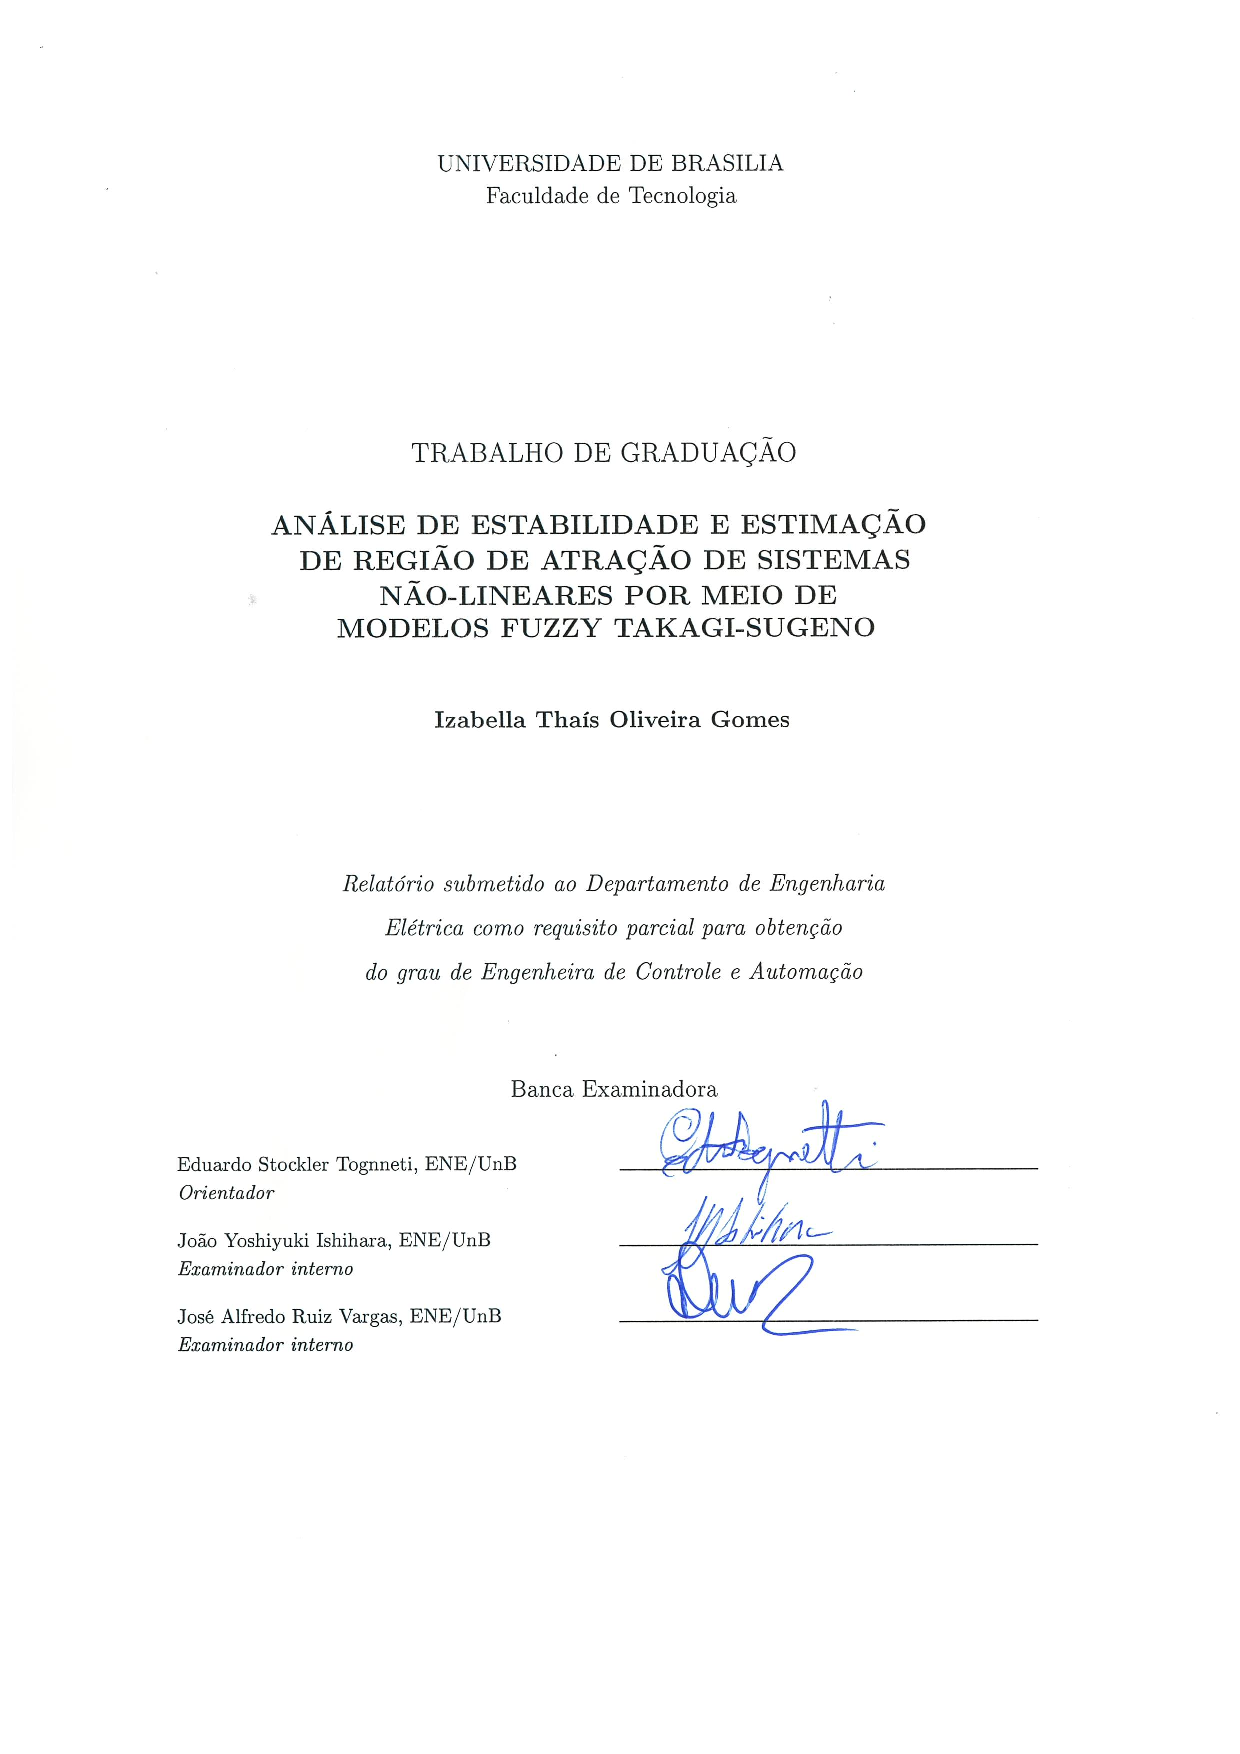
\includegraphics[width = 21cm]{contra-capa_tg_izabella-gomes_2017-2}

%%%%%%%%%%%%%%%%%%%%%%%%%%%%%%%%%%%%%%%%%%%%%%%%%%%%%%%%%%%%%%%%%%%%%%%%%
% Ficha catalográfica
%%%%%%%%%%%%%%%%%%%%%%%%%%%%%%%%%%%%%%%%%%%%%%%%%%%%%%%%%%%%%%%%%%%%%%%%%
\noindent \textbf{FICHA CATALOGRÁFICA}

\noindent %
\fbox{\begin{minipage}[t]{1\columnwidth}%
JOÃO, DA SILVA

Título do trabalho dividido em mais de uma linha para títulos realmente
longos como este,

\medskip{}


{[}Distrito Federal{]} 2015.

\medskip{}


x, 101p., 297 mm (FT/UnB, Engenheiro, Controle e Automação, 2015).
Trabalho de Graduação \textendash{} Universidade de Brasília.Faculdade
de Tecnologia.

\medskip{}


1. Bla\hfill{}2.Ble\hfill{}

3. Bli

\medskip{}


I. Mecatrônica/FT/UnB\hfill{}II. Título (Série)\hfill{}

%
\end{minipage}}

\noindent \medskip{}


\noindent \textbf{REFERÊNCIA BIBLIOGRÁFICA}

SILVA, JOÃO DA, (2015). Título do trabalho dividido em mais de uma
linha para títulos realmente longos como este. Trabalho de Graduação
em Engenharia de Controle e Automação, Publicação FT.TG-$n^{\circ}022$,
Faculdade de Tecnologia, Universidade de Brasília, Brasília, DF, 101p.

\noindent \bigskip{}


\noindent \textbf{CESSÃO DE DIREITOS}

\noindent AUTOR: João da Silva

TÍTULO DO TRABALHO DE GRADUAÇÃO: Título do trabalho dividido em mais
de uma linha para títulos realmente longos como este.

\noindent \medskip{}


\noindent GRAU: Engenheiro\hfill{}ANO: 2015\hfill{}

\noindent \medskip{}


É concedida à Universidade de Brasília permissão para reproduzir cópias
deste Trabalho de Graduação e para emprestar ou vender tais cópias
somente para propósitos acadêmicos e científicos. O autor reserva
outros direitos de publicação e nenhuma parte desse Trabalho de Graduação
pode ser reproduzida sem autorização por escrito do autor.

\noindent \bigskip{}


\noindent \rule[0.5ex]{1\columnwidth}{1pt}

\noindent João da Silva

\noindent Rua dos Bobos, nº 0, Bairro Feliz.

\noindent 71000-000 Brasília \textendash{} DF \textendash{} Brasil.


%%%%%%%%%%%%%%%%%%%%%%%%%%%%%%%%%%%%%%%%%%%%%%%%%%%%%%%%%%%%%%%%%%%%%%%%%
% Dedicatorias
%%%%%%%%%%%%%%%%%%%%%%%%%%%%%%%%%%%%%%%%%%%%%%%%%%%%%%%%%%%%%%%%%%%%%%%%%
\frontmatter


\dedicatoriaautori{Aos meus amados pais, Claudio e Tereza, e à minha amada irmã, Hellen.}

\dedicatoriaautorii{Dedicatória do autor 2}

\dedicatoriaautoriii{Dedicatória do autor 3}

\dedicatoria

%%%%%%%%%%%%%%%%%%%%%%%%%%%%%%%%%%%%%%%%%%%%%%%%%%%%%%%%%%%%%%%%%%%%%%%%%
% Agradecimentos
%%%%%%%%%%%%%%%%%%%%%%%%%%%%%%%%%%%%%%%%%%%%%%%%%%%%%%%%%%%%%%%%%%%%%%%%%
% Texto de agradecimentos do primeiro autor
\agradecimentosautori{Ao Deus que me sustenta e me capacita em todos os momentos, mesmo em meio às minhas limitações, eu agradeço. Ao meu orientador, Professor Dr. Eduardo Stockler Tognetti, obrigada por depositar em minhas mãos a missão de redigir este trabalho, por acreditar em meu potencial e por ser tão atencioso. Cada conversa, reunião, email respondido e cada explicação anotada em folhas de rascunho foram essenciais para a conclusão deste trabalho. Agradeço à Professora Dra Carla Denise Castanho, que me abriu tantas portas no início do meu curso de graduação, com quem tanto aprendi e em quem tanto me espelho. À minha amada amiga Letícia van der Ploeg, o maior presente que a graduação me trouxe, obrigada por ser minha companheira desde o primeiro até o último momento deste curso. Aos queridos amigos que granjeei durante o curso e que levo para a vida toda, obrigada por tornarem os desafios da universidade tão mais fáceis de serem enfrentados. Aos meus colegas de gestão na Mecajun, os momentos vividos junto a vocês me fizeram crescer pessoal e profissionalmente, obrigada. Aos meus amigos da UnBall, sentirei saudades dos momentos de descontração e do companheirismo que vivenciamos dentro e fora das competições. Às minhas amigas-irmãs Nayhane, Jhenefer e Raquel, às minhas amiguinhas Rauenya e Analine e à tia Silvana, obrigada por cada oração e por não desistirem de mim por eu ter que me ausentar tanto durante graduação. Aos meus pais e minha irmã, obrigada por viverem comigo cada batalha que tive que lutar durante a graduação, vocês são meu refúgio nos momentos de dificuldades.}

% Texto de agradecimentos do segundo autor. Caso não tenha um segundo autor, este texto não 
% será mostrado
\agradecimentosautorii{Não será necessário.}

% Texto de agradecimentos do segundo autor. Caso não tenha um terceiro autor, este texto não 
% será mostrado
\agradecimentosautoriii{Não será necessário.}

% Comando para criar a página de agradecimentos
\agradecimentos

%%%%%%%%%%%%%%%%%%%%%%%%%%%%%%%%%%%%%%%%%%%%%%%%%%%%%%%%%%%%%%%%%%%%%%%%%
% Resumo: arquivo resumo.tex editável no Scientific Word
%%%%%%%%%%%%%%%%%%%%%%%%%%%%%%%%%%%%%%%%%%%%%%%%%%%%%%%%%%%%%%%%%%%%%%%%%
%TCIDATA{LaTeXparent=0,0,relatorio.tex}
\setcounter{page}{1} \pagenumbering{roman} \pagestyle{plain}
%Essa bancada laboratorial cont�m dois tanques em uma parte alta e os outros dois em uma parte inferior, estando estes emparelhados com os de cima. H� um reservat�rio de �gua, duas bombas que transportam a �gua do reservat�rio para os tanques e v�lvulas ajust�veis entre as bombas e os tanques. Os tanques superiores drenam �gua diretamente para os tanques inferiores. Ess

\resumo{Resumo}{Este texto apresenta...}

\vspace*{2cm}
%
\resumo{Abstract}{
This text presents ...}

%%%%%%%%%%%%%%%%%%%%%%%%%%%%%%%%%%%%%%%%%%%%%%%%%%%%%%%%%%%%%%%%%%%%%%%%%
% Listas de conteúdo, figuras e tabelas.
%%%%%%%%%%%%%%%%%%%%%%%%%%%%%%%%%%%%%%%%%%%%%%%%%%%%%%%%%%%%%%%%%%%%%%%%%
\sumario
\listadefiguras
% \listadetabelas


%%%%%%%%%%%%%%%%%%%%%%%%%%%%%%%%%%%%%%%%%%%%%%%%%%%%%%%%%%%%%%%%%%%%%%%%%
% Lista de simbolos.
%%%%%%%%%%%%%%%%%%%%%%%%%%%%%%%%%%%%%%%%%%%%%%%%%%%%%%%%%%%%%%%%%%%%%%%%%
%TCIDATA{LaTeXparent=0,0,these.tex}


%\chapter*{\setfontarial\mdseries LISTA DE SÍMBOLOS} % se usar ft1unb.sty, descomente esta linha



\chapter*{LISTA DE SÍMBOLOS}

% se usar ft2unb.sty, descomente esta linha



\subsection*{Símbolos Latinos}

\begin{tabular}{p{0.1\textwidth}p{0.63\textwidth}>{\PreserveBacklash\raggedleft}p{0.15\textwidth}}
$v$  & Velocidade linear  & {[}m/s{]}\tabularnewline
\end{tabular}


\subsection*{Símbolos Gregos}

\begin{tabular}{p{0.1\textwidth}p{0.63\textwidth}>{\PreserveBacklash\raggedleft}p{0.15\textwidth}}
$\omega$ & Velocidade angular & {[}rad/s{]}\tabularnewline
\end{tabular}


\subsection*{Grupos Adimensionais}

\begin{tabular}{p{0.1\textwidth}p{0.8\textwidth}}
i, k & Contador\tabularnewline
\end{tabular}


\subsection*{Subscritos}

\begin{tabular}{p{0.1\textwidth}p{0.8\textwidth}}
$ref$  & referência \tabularnewline
$fer$  & ferramenta \tabularnewline
$sis$  & sistema \tabularnewline
$des$  & desejado\tabularnewline
\end{tabular}


\subsection*{Sobrescritos}

\begin{tabular}{p{0.1\textwidth}p{0.8\textwidth}}
$\cdot$  & Variação temporal \tabularnewline
$-$  & Valor médio \tabularnewline
\end{tabular}


\subsection*{Siglas}

\begin{tabular}{p{0.1\textwidth}p{0.8\textwidth}}
PCI  & \textit{Peripheral Component Interconnect}\tabularnewline
CPU & Unidade Central de Processamento - \textit{Central Processing Unit} \tabularnewline
AO & Saída Analógica - \textit{Analog Out}\tabularnewline
DO & Saída Digital - \textit{Digital Out}\tabularnewline
CS & Seletor de \textit{Chip - Chip Select}\tabularnewline
SC & Sem Conexão\tabularnewline
P.I. & Placa de Interface\tabularnewline
ICW & \textit{Initialization Command Words}\tabularnewline
OCW & \textit{Operational Control Word}\tabularnewline
\end{tabular}


%%%%%%%%%%%%%%%%%%%%%%%%%%%%%%%%%%%%%%%%%%%%%%%%%%%%%%%%%%%%%%%%%%%%%%%%%
% Corpo principal
%%%%%%%%%%%%%%%%%%%%%%%%%%%%%%%%%%%%%%%%%%%%%%%%%%%%%%%%%%%%%%%%%%%%%%%%%
\mainmatter
\setcounter{page}{1} \pagenumbering{arabic} \pagestyle{plain}

% *** Introducao ***

\chapter{Introdução}

\label{CapIntro}

% Resumo opcional. Comentar se não usar.
\resumodocapitulo{Resumo opcional}


\section{Contextualização}

Contextualizar.

Conforme \cite{article:dummy}, vide a Tabela \ref{tab:Descrever-tabela}.
Assim sendo, observe a Figura \ref{fig:Descrever-figura.}.
\begin{table}[h]
\begin{centering}
\begin{tabular}{|c|c|c|c|c|}
\hline
 &  &  &  & \tabularnewline
\hline
\hline
 &  &  &  & \tabularnewline
\hline
 &  &  &  & \tabularnewline
\hline
 &  &  &  & \tabularnewline
\hline
 &  &  &  & \tabularnewline
\hline
\end{tabular}
\par\end{centering}

\label{tab:Descrever-tabela}Descrever tabela.


\end{table}


\begin{figure}[h]
\begin{centering}

\includegraphics[width=0.4\columnwidth]{figs/capa_fundo}
\par\end{centering}

\label{fig:Descrever-figura.}Descrever figura.


\end{figure}



\section{Definição do problema}

Definir problema.


\section{Objetivos do projeto}

Objetivos.


\section{Resultados obtidos}

Resultados.


\section{Apresentação do manuscrito}

Apresentar.


% *** Modelagem de sistemas nãoilineares por fuzzy Takagi-Sugeno ***
%TCIDATA{LaTeXparent=0,0,relatorio.tex}
                      

\chapter{Modelagem fuzzy Takagi-Sugeno de sistemas não lineares}\label{cap_ModelagemSisNaoLinearesporFuzzyTS}

\section{Introdução}

Sistemas dinâmicos não lineares variantes no tempo modelam boa parte dos problemas encontrados nas mais diversas áreas da engenharia \cite{bookogata:2003}. A observação do comportamento deste tipo de sistema, dado uma condição inicial, permite análises qualitativas da estabilidade destes \cite{bookkhalil:2003}. Quantitativamente, porém, a determinação da região de estabilidade e a aplicação de técnicas de controle para este tipo de sistema não são triviais, justamente devido à natureza não linear que possuem. Assim, métodos matemáticos são utilizados  a fim de ser obter modelos lineares equivalentes a estes sistemas, os quais facilitem o uso de ferramentas existentes na literatura. Neste contexto, este capítulo, além de apresentar uma discussão sobre sistemas não lineares,  discorre também sobre o uso do retrato de fase como um meio de analisar qualitativamente o comportamento de sistemas não lineares e aborda a utilização de lógica fuzzy, segundo a proposto por Takagi e Sugeno \cite{articlets:1985},  para a modelagem local de sistemas não lineares.

\section{Análise qualitativa de sistemas não lineares} \label{Sist-nao-lin-retrato-fase}

Um sistema é dito não linear quando a ele não é  possível aplicar o princípio da superposição, ou seja, a resposta a duas entradas distintas não pode ser calculada tratando uma resposta por vez e depois somando os resultados \cite{bookogata:2003}. Mesmo com a enorme gama de sistemas físicos representados como dinâmica linear, a grande maioria destes possui dinâmica real não linear, por isso o estudo de sistemas desta natureza torna-se praticamente inevitável do ponto de vista da engenharia.

\subsection{Sistemas não lineares}

Sistemas não lineares podem ser descritos como o conjunto formado por um número finito de equações ordinárias diferenciais de primeira ordem na forma
\begin{equation}\label{sist_nao_linear_generico}
\mathbf{\dot{x}}=g\mathbf{(x,u)}
\end{equation}
onde $x \in \rm I\!R^n$ é o vetor de estados, $u \in \rm I\!R^n$ o vetor dos sinais de entrada. Estes sistemas podem ser representados na forma
\begin{equation}\label{eq:noninear_system}
\mathbf{\dot{x}} = \mathbf{A(x)x} + \mathbf{B(x)u}
\end{equation}
sendo $A(x) \in\rm I\!R^{n \times n}$ e $B(x) \in \rm I\!R^{n \times m}$ matrizes cujos elementos podem depender dos estados do sistema e os quais também são funções contínuas num certo domínio de interesse. Este tipo de representação pode ser não único, ou seja, podem ser escolhidos diferentes $\textbf{A(x)}$ e $\textbf{B(x)}$ a partir da mesma função $g\textbf{(x,u)}$, estas diferentes escolhas são feitas pelo projetista. A seguir é mostrado um exemplo de um sistema não linear $g(\textbf{x,u})$ para o qual se obtém mais de uma representação diferente para $\textbf{A(x)}$ e $\textbf{B(x)}$.

\begin{example}[Representações distintas de um mesmo sistema não linear] Considere o sistema não linear dado por
	\begin{equation*}
		g(\textbf{x,u}) = x_1^2x_2+u
	\end{equation*}
	Este sistema pode ser representado como
	\begin{equation*}
	\dot{\textbf{x}} = a(\textbf{x})x_2+b(\textbf{x})u,\quad a(\textbf{x}) = x_1^2,\quad b(\textbf{x}) = 1
	\end{equation*}
	De forma análoga, o sistema pode ser representado como
	\begin{equation*}
	\dot{\textbf{x}} = a(\textbf{x})x_1+b(\textbf{x})u,\quad a(\textbf{x}) = x_1x_2,\quad b(\textbf{x}) = 1
	\end{equation*}
	Desta maneira, é possível verificar que um mesmo sistema não linear pode ser representado de diferentes formas, que dependerão da escolha do projetista.
	\label{ex:nonlinear_system_multiple_representation}
\end{example}

Como em (\ref{eq:noninear_system}) o sistema não depende explicitamente do tempo, este é dito como um sistema autônomo invariante no tempo \cite{bookkhalil:2003}. Nos exemplos apresentados neste trabalho, o sinal de entrada $u$ não será explicitado, utilizando-se, assim, equações de estado não forçadas \cite{bookkhalil:2003}. Trabalhar com este tipo de equação de estado não necessariamente significa que a entrada é nula, mas pode ser que a entrada tenha sido especificada como uma função dependente do tempo, ou das variáveis de estado, ou de ambos, de forma que se elimine $u$, obtendo uma equação de estados não forçada. Assim, neste trabalho estaremos interessados na classe particular de sistemas não lineares descritos na forma
\begin{equation}\label{eq:nonlinear_system_f_x}
\dot{\textbf{x}} = f(\textbf{x})
\end{equation}
Que pode ser representada equivalentemente por
\begin{equation}\label{eq:nonlinear_system_mean_representation}
	f(\textbf{x})=\textbf{A}(\textbf{x})\textbf{x}
\end{equation}
Para os sistemas apresentados no decorrer deste trabalho, quando as equações de estado apresentarem sinal de entrada, este será definido como um sinal de valor constante fixo $\textbf{u}(t)=\textbf{u}^*$ para qualquer instante de tempo $t \geq 0$, de forma tal que sejam feitas manipulações matemáticas a fim de se obter o sistema na forma (\ref{eq:nonlinear_system_mean_representation}).

\subsection{Pontos de equilíbrio}\label{subsec_pontoEq}

A engenharia de controle tem como um dos principais desafios manter o sistema funcionando em uma faixa de operação denominada regime permanente. Um sistema opera em regime permanente quando as variáveis de estado se mantêm constantes a medida que o tempo passa. Estes valores constantes correspondem ao ponto de equilíbrio do sistema\cite{bookboydl:1994}. Assim, o comportamento de sistemas modelados por equações de estado, como o da equação \ref{eq:noninear_system}, é caracterizado quanto aos seus  pontos de equilíbrio.

Ponto de equilíbrio, segundo (Khalil, 2003)\cite{bookkhalil:2003}, é definido como um ponto $\mathbf{x = x^*}$ no espaço de estados tal que, seja qual for o ponto inicial $\mathbf{x_0}$ em relação a $\mathbf{x^*}$, o sistema sempre convergirá para $\mathbf{x^*}$, para qualquer instante de tempo futuro.
Os pontos de equilíbrio da equação (\ref{eq:nonlinear_system_f_x}) equivalem às suas raízes reais, tais que
\begin{equation}\label{eq:ponto_de_eq}
\mathbf{f(x)} = 0.
\end{equation}

Caso a equação \ref{eq:ponto_de_eq} possua mais de uma raiz real, pode-se definir uma vizinhança local para cada ponto de equilíbrio. Desta forma, se houver apenas um ponto de equilíbrio na vizinhança, diz-se que este é um ponto de equilíbrio isolado. Caso contrário, diz-se que a vizinhança possui uma continuidade de pontos de equilíbrio.

Por convenção, será assumido que o sistema (\ref{eq:nonlinear_system_f_x}) possui um único ponto de equilíbrio na região de interesse no plano de estados e este ponto sempre estará localizado na origem, sem perdas de generalidade, utilizando-se do artifício de mudança de variáveis, conforme descrito a seguir.

Suponha que o ponto de equilíbrio do sistema (\ref{eq:nonlinear_system_f_x}) seja $\textbf{x = x}^*$, tal que $\textbf{x}^* \neq \textbf{0}$. E considere a mudança de variáveis $\textbf{y = x - x}^*$. A derivada de $\textbf{y}$ é dada por
\begin{equation*}\mathbf{\dot{y} = \dot{x} = f(x) = f(y + x^*)}
 \myeq 
g(\textbf{y})
\end{equation*}
onde $g(\textbf{0}) = \textbf{0}$. Portanto, na nova variável $\textbf{y}$, o sistema tem ponto de equilíbrio na origem, sem que haja perda de generalidade.

\subsection{Retrato de fase} \label{subsec_phasePortrait}

Considerando o caso específico em que o sistema da equação (\ref{eq:nonlinear_system_f_x}) possui apenas duas variáveis de estado, ou seja, para sistemas de segunda ordem, é possível representar a curva de respostas destes em um plano. Assim, pode-se fazer uma análise qualitativa do comportamento do sistema, gerando-se a curva de resposta para $x_1$ e $x_2$ para instantes de tempo maiores que zero sobre o plano x1-x2, denominado plano de estados. As curvas de resposta são traçadas pela combinação de vetores tangenciais à resposta do sistema a partir de um dado ponto inicial $\mathbf{x_0}$.

Um mesmo sistema pode apresentar inúmeras curvas de resposta diferentes, cada uma oriunda de um ponto inicial $\mathbf{x_0}$ distinto. Para se obter uma representação mais próxima do comportamento real da curva de resposta de $\mathbf{f(x)}$ a partir de $\mathbf{x_0}$, fixam-se os módulos dos vetores tangenciais às respostas em um valor específico, conservando a direção e o sentido destes, de forma que sejam traçados vetores equidistantes sobre o plano de estados, até que se obtenha a curva de resposta.

A representação de todas as curvas de resposta sobre uma determinada região no plano de estados constitui o\textbf{ retrato de fase} do sistema\cite{bookkhalil:2003}. Desta maneira, o retrato de fase é obtido percorrendo-se o grid do plano x1-x2, de forma que, $\mathbf{x_0}$ será um novo ponto em x1-x2 para cada posição do grid e a trajetória da resposta é obtida para cada $\mathbf{x_0}$ distinto. A figura do retrato de fase do sistema permite apenas uma análise qualitativa deste, visto que, uma vez que o tempo é omitido ao se plotar as trajetórias, torna-se inviável obter a resposta $\mathbf{x(t)}$ associada a uma trajetória \cite{bookkhalil:2003}.

A análise qualitativa que se pode fazer a partir do retrato de fase está relacionada com a estabilidade dos pontos de equilíbrio do sistema. Portanto, faz-se importante escolher uma região do plano de estados tal que contenha todos, ou a maioria, destes pontos de equilíbrio.

Um ponto de equilíbrio será estável quando qualquer resposta iniciada próxima a este se mantém sempre próxima; e é instável, caso se afaste. A Figura \ref{fig:pontos_eq_retrato_fase}, ilustra exemplos de retrato de fase em torno de um ponto de equilíbrio estável e outro instável, onde o ponto de equilíbrio é representado na cor vermelha e as trajetórias de resposta que geram o retrato de fase em azul.

\begin{figure}[htbp]
	\centering
	\subfigure[ref1][Ponto de equilíbrio estável]{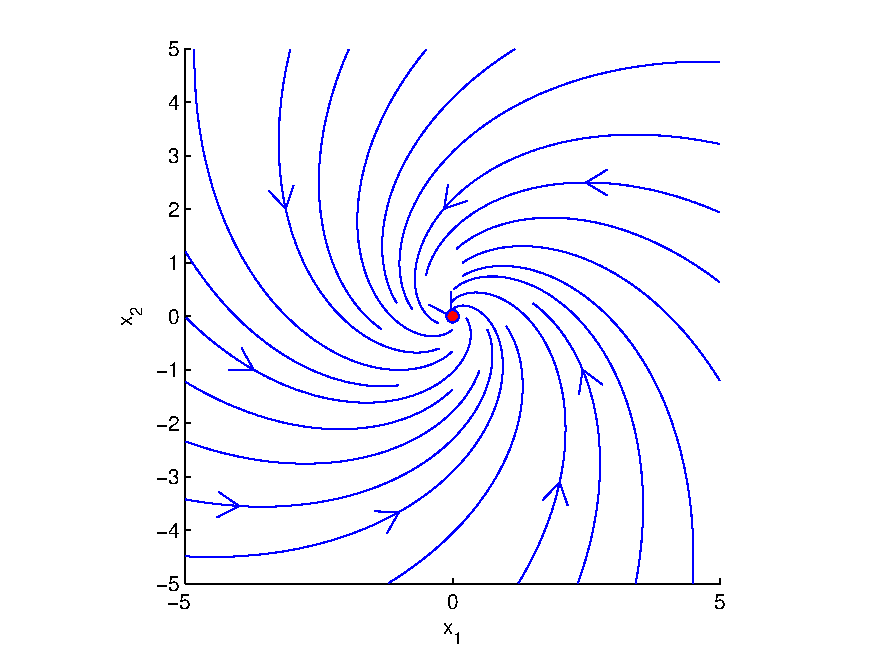
\includegraphics[width=7cm]{phase_portrait_stable}}
	\qquad
	\subfigure[ref2][Ponto de equilíbrio instável]{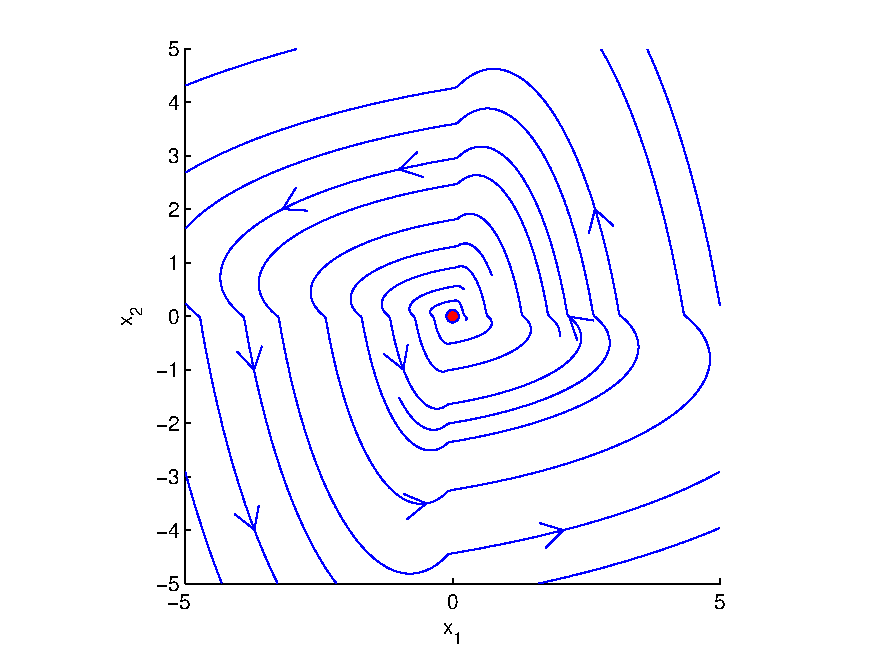
\includegraphics[width=7cm]{phase_portrait_unstable}}
	\caption{Retrato de fase para pontos de equilíbrio estável e instável}
	\label{fig:pontos_eq_retrato_fase}
\end{figure}

Além de estável e instável, o retrato de fase pode revelar outras configurações para os pontos de equilíbrio, como são os casos apresentados na Figura \ref{fig:outras_config_retrato_fase}, por exemplo.
No caso em que as trajetórias, além de se manter próximas ao ponto de equilíbrio, também convirjam a este quando o tempo tende ao infinito, o ponto de equilíbrio é dito como assintoticamente estável, como mostra a Figura \ref{fig:outras_config_retrato_fase} (a).
Já a Figura \ref{fig:outras_config_retrato_fase} (b) ilustra o caso em que as trajetórias se aproximam do ponto de equilíbrio a partir de determinados pontos iniciais e em seguida se afastam, mas sem nunca atingirem o ponto de equilíbrio. Este tipo de comportamento caracteriza o ponto de equilíbrio como um ponto de sela. 

\begin{figure}[htbp]
	\centering
	\subfigure[ref1][Ponto de equilíbrio  assintoticamente estável]{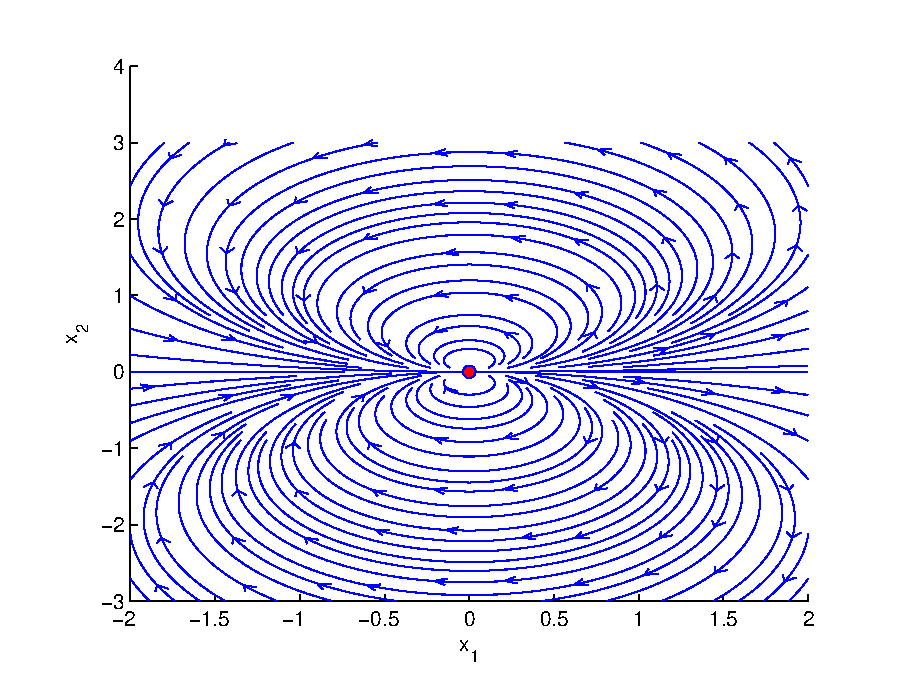
\includegraphics[width=7cm]{phase_portrait_assimptotically_stable}}
	\qquad
	\subfigure[ref2][Ponto de equilíbrio como ponto de sela]{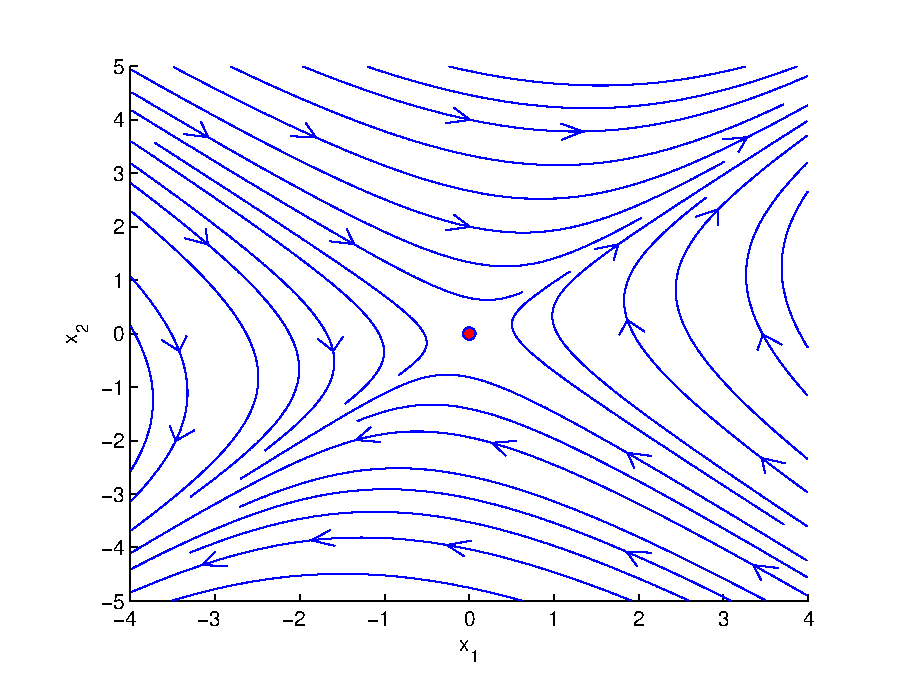
\includegraphics[width=7cm]{phase_portrait_saddle}}
	\caption{Retrato de fase para pontos de equilíbrio  assintoticamente estável e ponto de sela}
	\label{fig:outras_config_retrato_fase}
\end{figure}

Para o caso em que se tem um sistema de terceira ordem, cujo sistema não linear possui três variáveis de estado, também é possível obter o retrato de fase. O plano de estados passa a ser tridimensional e cada ponto terá três componentes: $\mathbf{x_1}$, $\mathbf{x_2}$ e $\mathbf{x_3}$. A partir daí a ideia passa a ser a mesma descrita para sistemas de segunda ordem.

Os próximos capítulos abordarão métodos de verificação de estabilidade de sistemas não lineares e a obtenção da região em que a estabilidade é garantida. Assim, será possível utilizar o retrato de fase como um meio de validar a região de estabilidade, visto que o retrato de fase é uma aproximação bastante realista do comportamento do sistema ao longo do tempo para diversos pontos iniciais \cite{bookkhalil:2003}.

\subsection{Exemplos} \label{subsection:descr_exemplos}

Nesta seção serão apresentados os exemplos utilizados nas análises e validações dos tópicos discutidos no decorrer deste trabalho. O primeiro exemplo consiste em um sistema não linear de segunda ordem retirado do artigo publicado por Lee, Park an Joo em 2011\cite{article:LPJ:2011}. Em seguida, tem-se um sistema de terceira ordem, que equivale ao modelo de um inversor de tensão conectado a um barramento de corrente alternada infinito. Por fim, o terceiro exemplo apresentado, um sistema  de quarta ordem, corresponde ao modelo do processo  de quatro tanques não linear disponibilizado nas instalações do Laboratório de Automação e Robótica da Universidade de Brasília (LARA - UnB).

\begin{example}
[Sistema não linear de segunda ordem \cite{article:LPJ:2011}] Considere o sistema não linear de segunda ordem descrito por
\begin{equation*}
\mathbf{ \begin{bmatrix}\dot{x_1}\\ \dot{x_2} \end{bmatrix} = \begin{bmatrix} -2 & 4\\  -1 - \dfrac{\lambda (1 - sen(x_1))}{2} & -2 \end{bmatrix} \begin{bmatrix}x_1 \\ x_2 \end{bmatrix}}
\end{equation*}
onde $\lambda$ é um escalar e $\mathbf{C_1 = \{x(t) \in \rm I\!R^n | |x_i(t)| \leq \pi/2, i \in \{1,2\}\}}$. Inicialmente, será assumido que $\lambda = 20$.
\label{example_LPJ12}
\end{example}

Para se obter o retrato de fase deste sistema, primeiramente deve-se encontrar os pontos de equilíbrio, que correspondem à solução do sistema para $\dot{x}_1$ = 0 e $\dot{x}_2$ = 0. Neste caso, verifica-se que o sistema possui um único ponto de equilíbrio\footnote{para obter os pontos de equilíbrio utilizou-se a função \textit{fsolve} do Matlab, que retorna o vetor \textbf{x} correspondente à solução da equação \textbf{f(x) = 0}.}$^,$\footnote{$x^*\triangleq x(0)$} dado por
\begin{equation*}
\mathbf{
\begin{bmatrix}x^*_1\\x^*_2\end{bmatrix} = \begin{bmatrix}0\\0\end{bmatrix}}
\end{equation*}

O retrato de fase do sistema corresponde às trajetórias obtidas assumindo-se diferentes pontos iniciais sobre do plano de estados limitado pela região contida no domínio de ${x_1}$ e ${x_2}$ e é apresentado na Figura \ref{fig:retrato_fase_ex2_LPJ12}.

\begin{figure}[htbp]
	\centering
	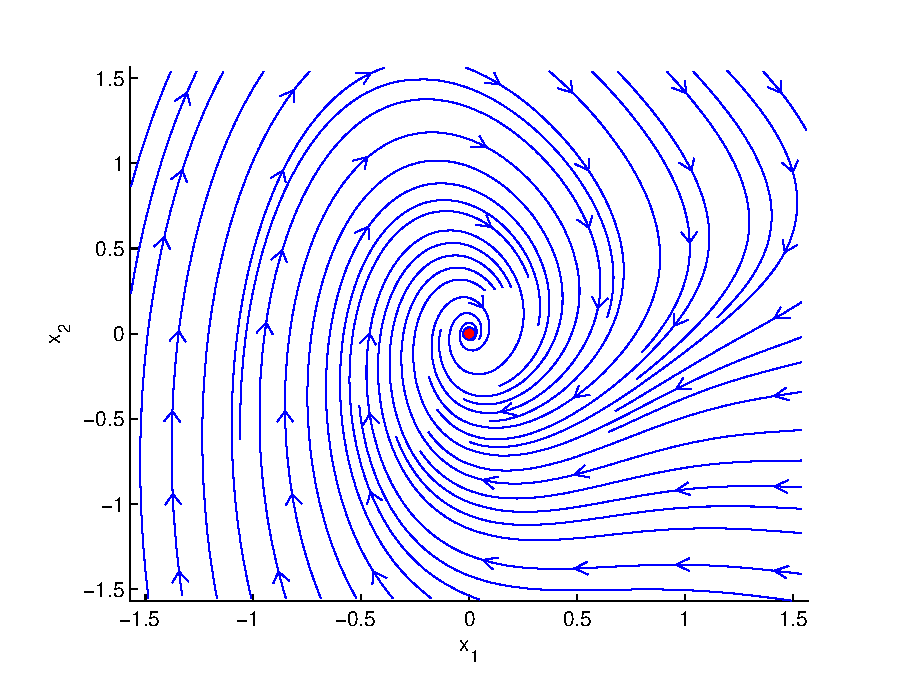
\includegraphics[width=10cm]{phase_portrait_ex2_LPJ12}
	\caption{Retrato de fase do sistema de segunda ordem do Exemplo \ref{example_LPJ12}. As trajetórias das respostas para os diferentes pontos iniciais estão representadas em azul e o ponto de equilíbrio aparece em vermelho.}
	 \label{fig:retrato_fase_ex2_LPJ12}
\end{figure}

O retrato de fase apresentado na Figura \ref{fig:retrato_fase_ex2_LPJ12} evidencia que o ponto de equilíbrio do sistema é assintoticamente estável, uma vez que todas as trajetórias de resposta para diferentes pontos iniciais dentro do domínio de \textbf{x} são atraídas para o ponto de equilíbrio.

\begin{example} [Sistema \textit{Droop}] O sistema proposto neste exemplo baseia-se no problema de controle de frequência e potência ativa para sistemas, que é definido pela dependência existente entre essas duas grandezas. A alteração da frequência afeta diretamente a potência ativa do sistema, Assim, reguladores de velocidade, ou de inclinação, são utilizados para prover o devido carregamento de sistemas interconectados.

Neste contexto, assuma um inversor de tensão de módulo $E_i$ e fase $\delta_i$ conectado a um barramento CA infinito com tensão de módulo $E_o$ e fase $0^{\circ}$ através de uma impedância de saída com módulo $Z_{oi}$ e fase $\theta_i$, conforme mostra a Figura \ref{fig:inversor_CA}.

\begin{figure}[htbp]
	\centering
	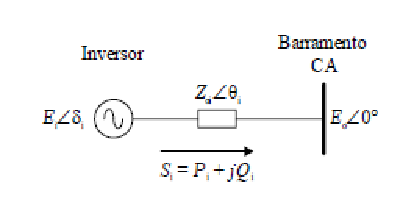
\includegraphics[width=6cm]{barramento}
	\caption{Inversor conectado a um barramento CA infinito}
	 \label{fig:inversor_CA}
\end{figure}

A potência aparente entregue pelo inversor ao barramento infinito, na forma retangular, é dada por
\begin{equation}
S_i = E_o(\dfrac{E_i\cos(\delta_i)-E_o+jE_i\sin(\delta_i)}{Z_{oi}\cos(\theta_i)+jZ_{oi}\sin(\theta_i)}).
\end{equation}
Separando-se  a parte real e a parte imaginária, definem-se as contribuições de potência ativa e reativa do inversor para o barramento CA, tal que
\begin{equation}\label{P_ativ}
P_i = (\dfrac{E_iE_o}{Z_{oi}}\cos(\delta_i)- \dfrac{E_o^2}{Z_{oi}})\cos(\theta_i)+\dfrac{E_iE_o}{Z_{oi}}\sin(\delta_i)\sin(\theta_i),
\end{equation}
\begin{equation}\label{P_reativ}
Q_i = (\dfrac{E_iE_o}{Z_{oi}}\cos(\delta_i)- \dfrac{E_o^2}{Z_{oi}})\sin(\theta_i)+\dfrac{E_iE_o}{Z_{oi}}\sin(\delta_i)\cos(\theta_i).
\end{equation}\label{P_i}
Quando a impedância de saída do inversor é resistiva, de modo que $\theta_i = 0$ e $Z_{oi} = R_{oi}$, então as expressões \ref{P_ativ} e \ref{P_reativ} podem ser rescritas como
\begin{equation}
P_i = \dfrac{E_iE_o\cos(\delta_i)- E_o^2}{R_{oi}},
\end{equation}
\begin{equation}\label{Q_i}
Q_i = -\dfrac{E_iE_o\sin(\delta_i)}{R_{oi}}.
\end{equation}
Considerando um ângulo de defasagem muito pequeno ($\delta_i \simeq 0$), as equações \ref{P_i} e \ref{Q_i} podem ser simplificadas considerando-se $\sin(\delta_i)\simeq\delta_i$ e $\cos(\delta_i)\simeq 1$.
\begin{equation}
P_i = \dfrac{E_iE_o- E_o^2}{R_{oi}},
\end{equation}
\begin{equation}
Q_i = -\dfrac{E_iE_o\delta_i}{R_{oi}}.
\end{equation}
Além disso, assumindo-se $Pi\sim E_i$ e $Q_i\sim -\delta_i$, tem-se as leis de controle do método \textit{Droop} convencional para a impedância de saída resistiva dadas por
\begin{equation}
E_i = E^*-n_i(P_i-P_i^*),
\end{equation}
\begin{equation}\label{lei_contr}
\omega_i = \omega^* + m_i(Q_i - Q^*).
\end{equation}
onde $E^*$ é a tensão de referência, $\omega^*$ é a frequência angular de referência, $P_i^*$ é a potência ativa de referência e $Q_i^*$ é a potência reativa de referência.

O coeficiente $n_i$ é geralmente determinado pela variação de tensão desejada para uma determinada variação de potência ativa, conforme a expressão
\begin{equation}
n_i = \dfrac{\Delta E_i}{\Delta P_i}.
\end{equation}
De modo semelhante, o coeficiente $m_i$ é determinado pela variação de frequência desejada para uma determinada variação de potência reativa, de acordo com a equação
\begin{equation}
m_i = \dfrac{\Delta \omega_i}{\Delta Q_i}.
\end{equation}
Assumindo, então, que os algoritmos de cálculo de $P_i$ e $Q_i$ possam ser modelados por um filtro passa-baixas de primeira ordem, tem-se
\begin{equation}
P_{f_i} = \dfrac{\omega_{pb}}{s+\omega_{pb}}P_i,
\end{equation}
\begin{equation}
Q_{f_i} = \dfrac{\omega_{pb}}{s+\omega_{pb}}Q_i.
\end{equation}
Equações tais que equivalem a
\begin{equation}
\dfrac{dP_{f_i}}{dt} = -\omega_{pb}P_{f_i}+\omega_{pb}P_i,
\end{equation}
\begin{equation}
\dfrac{dQ_{f_i}}{dt} = -\omega_{pb}Q_{f_i}+\omega_{pb}Q_i.
\end{equation}
Sabendo ainda que o ãngulo $\delta_i$ é obtido integrando-se a frequência $\omega_i$ a partir da lei de controle \ref{lei_contr}, pode-se escrever
\begin{equation}
\dfrac{d\delta_i}{dt} = m_i(Q_{f_i} - Q_i^*).
\end{equation}

Inibindo-se o termo subscrito $i$ das variáveis, considerando-se $\omega_{pb} = \omega_f$ e assumindo $Q_i^* = Q_{ref}$, $E_i^* = E_{ref}$ e $P_i^* = P_{ref}$, o modelo do sistema é obtido conforme segue.
\begin{equation} \label{eq:sist_droop}
\begin{cases}\dot{P}_f = -\omega_f P_f+\dfrac{\omega_f(V(E_{ref}-n(P_f-P_{ref}))\cos(\delta)-V^2)}{R_o}\\
\dot{Q}_f=
-\omega_f Q_f-
\dfrac{\omega_f V(E_{ref}-n(P_f - P_{ref}))\sin(\delta)}
{R_o}\\
\dot{\delta}=m(Qf-Q_{ref})\end{cases}
\end{equation}
Onde, $\omega_ f = 2\cdot\pi\cdot60 \dfrac{rad}{s}$, 
$V = 311 V$, 
$E_{ref} = 311 V$, 
$m = \dfrac{3.77}{22000} \dfrac{m}{s VAR}$, 
$n = \dfrac{20}{22000} \dfrac{m}{s W}$, 
$R_o = 0.1 \Omega$, 
$P_{ref} = 22000 W$ e 
$Q_{ref} = 0 VAR$.

As variáveis de estado são limitadas, tais que $C = \{x(t) \in \rm I\!R^3 | x_1(t) = P_f \in [0; 25000], x_2(t) = Q_f \in [-70000; 5000], x_3(t) = \delta \in [-0.02; 0.1]\}$.
\end{example}\label{ex:droop_UFSM}

Para se obter os pontos de equilíbrio do sistema, faz-se $\dot{\textbf{x}}(t) = 0$. Desta maneira, tem-se os pontos de equilíbrio
\begin{equation*}
\begin{bmatrix}x^*_1\\x^*_2\\x^*_3\end{bmatrix} = \begin{bmatrix}1.6252e+04\\0\\N*\pi\end{bmatrix}
\end{equation*}
em que $N = 0, 1, 3, ... 5$. Porém, dado que a variável de estado $x_3(t) = \delta$ é limitada no intervalo $[-0.02; 0.1]$, o único valor de $N$ que satisfaz esta limitação é $N = 0$. Assim, o ponto de equilíbrio do sistema a ser considerado é $\textbf{x}^* = \begin{bmatrix}1.6252e+04&0&0\end{bmatrix}'$.

Escolhendo-se arbitrariamente o ponto inicial $x_{inicial} = \begin{bmatrix}10000&1000&0.01\end{bmatrix}'$, obtemos a trajetória da resposta do sistema a partir deste ponto, conforme mostra a Figura \ref{fig:resp_droop}

\begin{figure}[htbp]
	\centering
	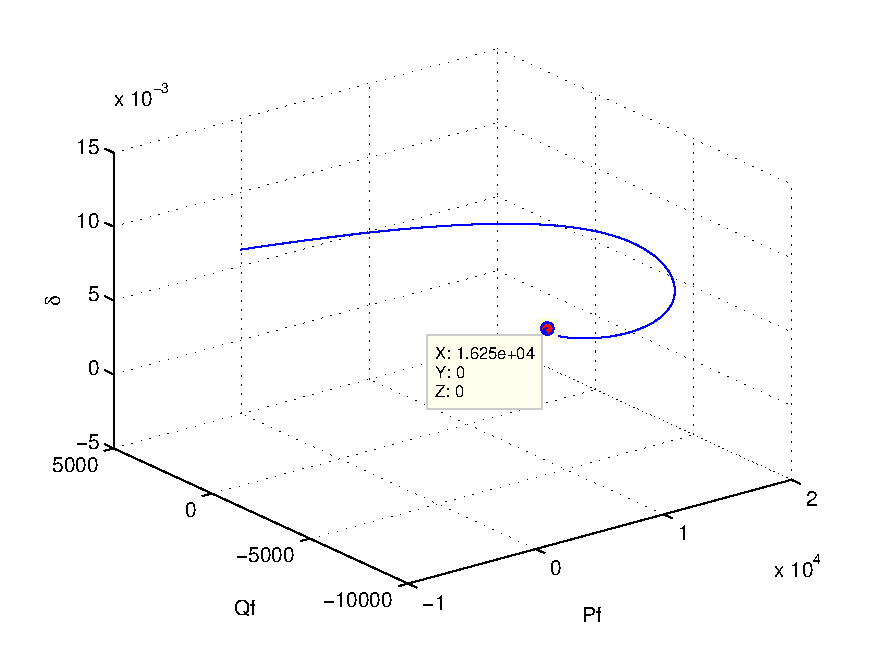
\includegraphics[width=10cm]{droop_answer_to_arbitrary_initial_value}
	\caption{Trajetória da resposta do sistema droop para o ponto inicial $x_{inicial} = [10000\quad1000\quad0.01]'$. A curva em azul corresponde à trajetória da resposta, enquanto o ponto em vermelho equivale ao ponto de equilíbrio do sistema}
	 \label{fig:resp_droop}
\end{figure}

Para este ponto inicial, é possível notar que a trajetória converge para o ponto de equilíbrio, sendo este um ponto de equilíbrio estável.

Ao se varrer um conjunto de pontos iniciais dentro da região representada pelos limites das variáveis de estado, é possível obter as  trajetórias de resposta do sistema a partir de cada ponto inicial. A Figura \ref{fig:droop_trajetorias} mostra estas trajetórias obtidas da varredura desta região para diferentes pontos iniciais.

\begin{figure}[htbp]
	\centering
	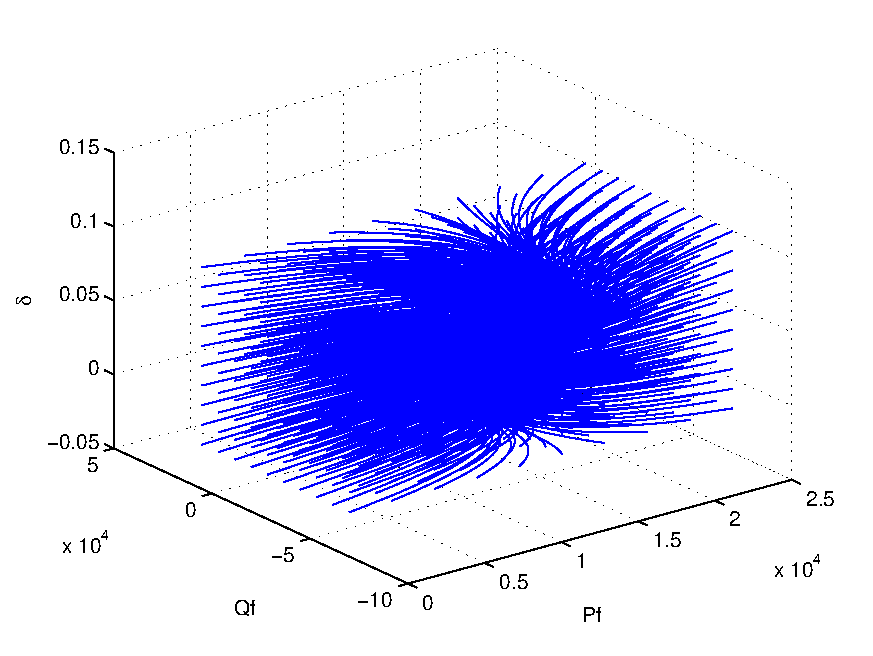
\includegraphics[width=10cm]{droop_answers_trajectories}
	\caption{Trajetórias de respostas do sistema para diferentes pontos iniciais definidos dentro da região contida pelos limites das variáveis de estado}
	 \label{fig:droop_trajetorias}
\end{figure}

Embora não seja claro enxergar na Figura \ref{fig:droop_trajetorias}, a simulação realizada para gerar esta imagem permitiu comprovar que todas as trajetórias obtidas a partir da variação dos pontos iniciais convergiram para o ponto de equilíbrio, constatando-se, de fato, que o ponto de equilíbrio  do sistema na região limitada pelas restrições das variáveis de estado é um ponto de equilíbrio estável.

Como neste trabalho se trabalhará com sistemas cujo ponto de equilíbrio encontra-se na origem, será utilizada mudança de variável $\mathbf{x_d = x - x^*}$ para deslocar o ponto de equilíbrio $\textbf{x}^* = \begin{bmatrix}1.6252e+04&0&0\end{bmatrix}'$ para a origem, tal que $\textbf{x}_d^* = \begin{bmatrix}0&0&0\end{bmatrix}'$ seja o ponto de equilíbrio deslocado do sistema, sem que haja perda de generalidade.

Assim, as variáveis de desvio serão
\begin{equation*}
\begin{bmatrix}x_{d_1}\\x _{d_2}\\x_{d_3}\end{bmatrix} = \begin{bmatrix}x_1\\x_2\\x_3\end{bmatrix} - \begin{bmatrix}x_1^*\\x_2^*\\x_3^*\end{bmatrix}
\end{equation*}

Assim, os novos limites das variáveis de estados são representados pela região poliédrica $C_1 = \{x_d(t) \in \rm I\!R^3 | x_{d1}(t) = P_f - x_1^* \in [-1.6252e+04; 25000 - 1.6252e+04], x_{d2}(t) = Q_f - x_2^* = Q_f \in [-70000; 5000], x_{d3}(t) = \delta -  x_3^* = \delta \in [-0.02; 0.1]\}$

Como o $x_1^* = 1.6252 \cdot10^{+4}$, $x_2* = 0$ e $x_3* = 0$, então $x_1 = x_{1_d} + x_1^*$, $x_{d_2} = x_2$ e $x_{d_3} = x_3$. Além disso, $\dot{x}_{d_1} = \dot{x}_1$, $\dot{x}_{d_2} = \dot{x}_2$ e $\dot{x}_{d_3} = \dot{x}_3$. Portanto, o sistema em função das variáveis de desvio é descrito conforme mostra a equação \ref{eq:sist_droop_var_desv}.
\begin{equation}\label{eq:sist_droop_var_desv}
\begin{cases}\dot{x}_{d_1} = -\omega_f x_{d_1} - \dfrac{\omega_f Vnx_{d_1}\cos(x_3)}{R_o} + \dfrac{\omega_f V(E_{ref} - n(x_1^* - P_{ref}))\cos(x_3)}{R_o} - \omega_f(x_1^* - \dfrac{V^2}{R_o})\\
\\\dot{x}_{d_2} = - \omega_fx_2 + \dfrac{\omega_fVnx_{d_1}\sin(x_3)}{R_o} - \dfrac{\omega_fV(E_{ref} - n(x_1^* - P_{ref}))\sin(x3)}{R_o}\\
\\\dot{x}_{d_3} = m(x_2 - Q_{ref})\end{cases}
\end{equation}

O sistema apresentado na equação \ref{eq:sist_droop_var_desv} possui ponto de equilíbrio na origem do plano de estados. Assumindo o ponto inicial $\textbf{x}_{d_{inicial}} = \begin{bmatrix}10000 - 1.6252e+04&1000&0.01\end{bmatrix}' = \begin{bmatrix}-6252&1000&0.01\end{bmatrix}'$, para fins de comparação com a Figura \ref{fig:resp_droop}. A curva de resposta para o sistema em função das variáveis de desvio para este ponto inicial é mostrada na Figura \ref{fig:resp_droop_var_desvio}.

\begin{figure}[htbp]
	\centering
	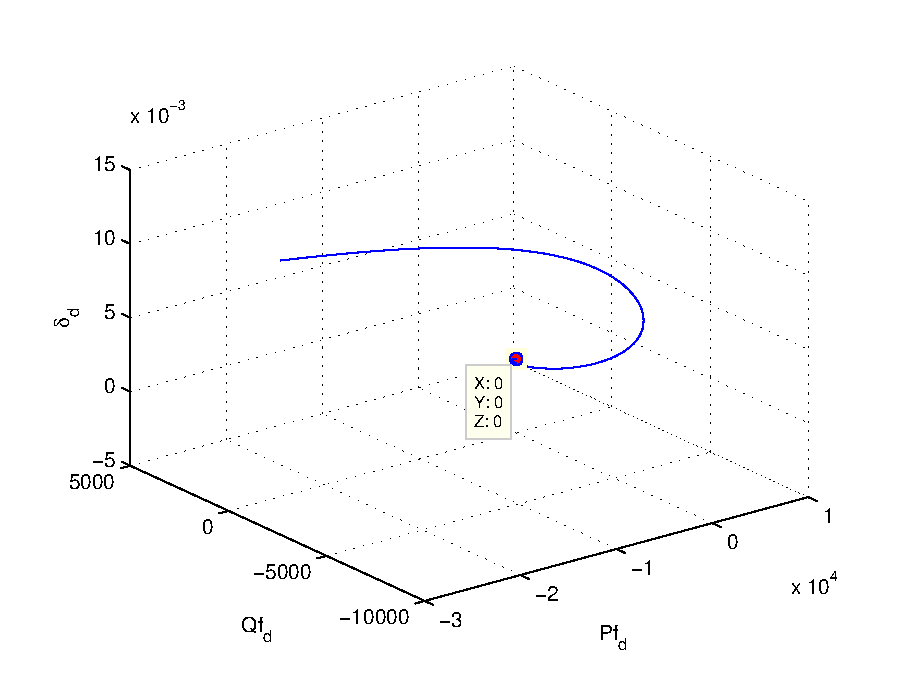
\includegraphics[width=10cm]{droop_answer_to_arbitrary_initial_value_var_desv}
	\caption{Trajetória da resposta do sistema droop para o ponto inicial $x_{d_{inicial}} = [-6252\quad1000\quad0.01]'$. A curva em azul corresponde á trajetória da resposta, enquanto o ponto em vermelho equivale ao ponto de equilíbrio do sistema}
	 \label{fig:resp_droop_var_desvio}
\end{figure}

Observe que o mesmo com o sistema redefinido para as varáveis de desvio, o comportamento do sistema continuou o mesmo, porém agora convergindo para a origem, a qual corresponde ao novo ponto de equilíbrio do sistema com variáveis de desvio.

\begin{example}
[Processo de quatro tanques] O processo de quatro tanques, foi introduzido por Johansson \cite{article:johansson:2000} e atualmente é utilizado como objeto de estudo em diversas universidades ao redor do mundo, pois permite o estudo de modelagem, linearização e projeto de controladores para sistema não linear multivariável \cite{article:roinila:2008}. A Figura \ref{fig:processo4tanques} traz uma representação do processo de quatro tanques.

\begin{figure}[htbp]
	\centering
	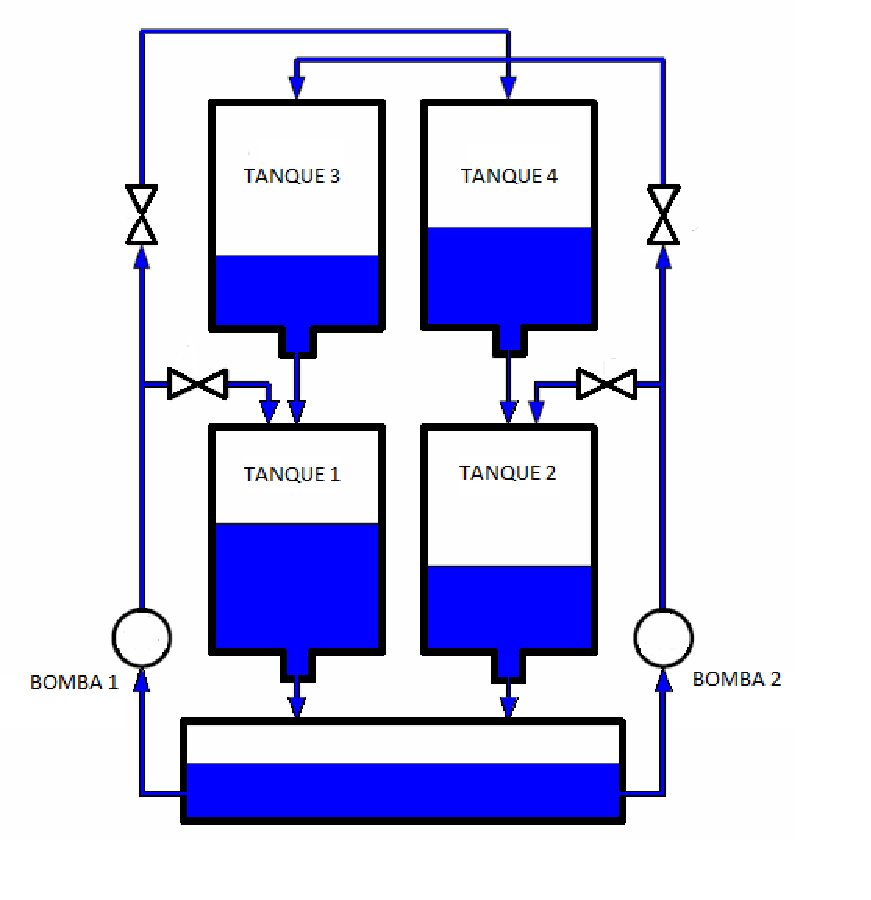
\includegraphics[width=8cm, height = 8cm]{4tanks}
	\caption{Diagrama esquemático do processo de quatro tanques}
	 \label{fig:processo4tanques}
\end{figure}

O objetivo deste processo é controlar os níveis dos tanques inferiores, tanques 1 e 2, utilizando-se as bombas 1 e 2. Assim, as entradas do processo são as tensões de entrada das bombas 1 e 2, que serão chamadas de $\upsilon_1$ e $\upsilon_2$, respectivamente. Já as saídas correspondem às tensões de medição dos níveis dos tanques 1 e 2. A partir destas tensões, é possível obter os níveis dos tanques propriamente ditos. Assim, as saídas correspondem ao nível $h_1$ do tanque 1 e ao nível $h_2$ do tanque 2.

A dinâmica deste processo é dita multivariável, pois cada uma das bombas afeta ambos os níveis $h_1$ e $h_2$ dos tanques 1 e 2. O acionamento da bomba 1 faz com que os tanques 1 e 4 sejam abastecidos e o tanque 4, por sua vez, despeja o líquido no tanque 2. De forma análoga, a bomba 2 abastece os tanques 2 e 3 e o tanque 3 despeja líquido no tanque 1.
A porcentagem do fluxo de líquido que vai para cada tanque está diretamente relacionada com a abertura das válvulas anteriores a estes. Esta proporção, ou taxa de líquido desviado para o tanque $i$, em que $i = 1, 2, 3, 4$, será representada pelo símbolo $\gamma_i$. Assim, a taxa de líquido desviado para o tanque $1$ será $\gamma_1$ e assim sucessivamente. Além disso, o volume de líquido em cada tanque será representado por $V_i$.

Dito isto, para obter a modelagem matemática do sistema, será considerado que o líquido utilizado no processo é água e será utilizada a equação de Bernoulli para líquidos incompressíveis
\begin{equation}\label{eq:Bernoulli}
 \dfrac{\rho \cdot v_i^2}{2} + \rho  \cdot g  \cdot h_i + P = constante 
\end{equation}
onde $\rho$ é a massa específica da água, $v_i$ é a velocidade de escoamento da água no tanque $i$, $g$ é a aceleração da gravidade, $h_i$ é a altura do nível do tanque $i$ e $P$ é a pressão. Além disso, utiliza-se o princípio de conservação de massa
\begin{equation}\label{eq:cons_massa}
\dot{V}_i = A_i  \cdot \dot{h}_i = q_{in} - q_{out} 
\end{equation}
em que $\dot{V}_i$ é a variação do volume de água do i-ésimo tanque, $A_i$ é a área da seção transversal e $\dot{h}_i$ é a variação da altura do nível do tanque $i$ ao longo do tempo. $q_{in}$ e $q_{out}$ são, respectivamente, os fluxos de entrada e de saída de água no tanque.

Assumindo a velocidade de escoamento $v_i$ na superfície da água é nula e que a altura $h_i$ do nível de água no tanque $i$ na parte inferior de cada tanque é zero, tem-se a equação de Bernoulli para a superfície da água tal que
\begin{equation}\label{eq:Bernoulli_sup}
 \rho  \cdot g  \cdot h_i + P = constante
\end{equation}

Já no fundo do tanque, a equação de Bernoulli será
\begin{equation}\label{eq:Bernoulli_fundo}
 \dfrac{\rho \cdot v_i^2}{2} + P = constante 
\end{equation}

Igualando as equações (\ref{eq:Bernoulli_sup}) e (\ref{eq:Bernoulli_fundo}), obtém-se a velocidade de escoamento da água
\begin{equation}\label{eq:vel_escoamento}
 v_i = \sqrt{g \cdot h_i} 
\end{equation}

O fluxo de saída do tanque é definido como o produto da velocidade de escoamento da água pela área da seção transversal $a_i$ da saída do tanque $i$. Já o fluxo de entrada se relaciona diretamente com o ganho de cada bomba e as tensões de entrada aplicadas \cite{inproc:arthur:2015}. Portanto as equações que regem o funcionamento do sistema são apresentadas as seguir, onde $\dot{h}_i$ é a variação da altura do tanque $i$ , $h_i$ é a altura do tanque $i$ e  $\upsilon_i$ é a tensão de entrada na bomba $i$ em um determinado instante de tempo, $ i = 1, 2, 3, 4$ e $j = 1, 2$.

\begin{equation*}
\begin{bmatrix}\dot{h_1}\\\dot{h_2}\\\dot{h_3}\\\dot{h_4}\end{bmatrix} = 
\begin{bmatrix}-\dfrac{a_1}{A_1}\cdot \dfrac{\sqrt{2\cdot g \cdot h_1}}{h_1}&0
&\dfrac{a_3}{A_1}\cdot \dfrac{\sqrt{2\cdot g \cdot h_3}}{h_3}&0
\\0&-\dfrac{a_2}{A_2}\cdot \dfrac{\sqrt{2\cdot g \cdot h_2}}{h_2}
&0&\dfrac{a_4}{A_2}\cdot \dfrac{\sqrt{2\cdot g \cdot h_4}}{h_4}
\\0&0&-\dfrac{a_3}{A_3}\cdot \dfrac{\sqrt{2\cdot g \cdot h_3}}{h_3}&0
\\0&0&0&-\dfrac{a_4}{A_4}\cdot \dfrac{\sqrt{2\cdot g \cdot h_4}}{h_4}\end{bmatrix}
\begin{bmatrix}h_1\\h_2\\h_3\\h_4\end{bmatrix}+\end{equation*}
\begin{equation}\label{eq:4tanques_matrix}
\begin{bmatrix}\dfrac{\gamma_1}{A_1}k_1&0\\0&\dfrac{\gamma_2}{A_2}k_2
\\0&\dfrac{1 - \gamma_2}{A_3}k_2\\\dfrac{1 - \gamma_1}{A_4}k_1\end{bmatrix}
\begin{bmatrix}\upsilon_1\\\upsilon_2\end{bmatrix}
\end{equation}

Como restrição física da planta disponibilizada no laboratório, a altura do volume de água em cada um dos tanques é limitada na região contida por $[0, 23 cm]$, de forma que quando o tanque estiver totalmente cheio, a altura do volume de água será de $23 cm$. As áreas da seção transversal é igual para todos os tanques e equivale a $A_i = 47.6 cm^2$. Os ganhos $k_1$ e $k_2$ das bombas são, respectivamente, 8.63 e 12.72, cuja unidade física é $cm^2/ V \cdot s$. Considerou-se a aceleração da gravidade como sendo $978 cm/s^2$. As áreas das seções transversais de saída dos tanques em $cm^2$ equivalem a $a_1 = 0.071$, $a_2 = 0.057$, $a_3 = 0.071$ e $a_4 = 0.057$.
\label{example_4tanques}
\end{example}

Para este exemplo, assumiremos que as entradas terão valor unitário, ou seja, $\begin{bmatrix}\upsilon_1&\upsilon_2\end{bmatrix}' = \begin{bmatrix}1&1\end{bmatrix}'$. Será assumido também que a altura estacionária dos níveis dos tanques será $ h^* = \begin{bmatrix}8.9\quad&9.97\quad&8.65\quad&9.67\quad\end{bmatrix}' cm$ \cite{inproc:arthur:2015}.Como este sistema possui quatro variáveis de estado, a representação do retrato de fase não é possível.

\section{Modelagem fuzzy}\label{Modelo-fuzzy}

Lógica fuzzy \cite{techreport:seatle}, ou lógica nebulosa, é um conceito que surgiu com uma forma de processar dados, possibilitando a associação de conjuntos parciais, ou seja, de conjuntos que têm uma determinada faixa de probabilidade de aderir a um conceito esperado. Definida originalmente na literatura por Lotfi A. Zadeh \cite{article:zadeh:1990}, a lógica fuzzy permite tratar sistemas nebulosos de forma quantitativa. Esta abordagem consiste em obter os graus de associação de cada elemento $\mathbf{x}$ na configuração fuzzy, atribuídos por uma função de associação $\mathbf{\alpha(x)}$, a qual corresponde a um valor definido em $\mathbf{x}$ e está contida no intervalo [0, 1].

Quanto maior o valor de $\mathbf{\alpha(x)}$, maior o grau de associação de $\mathbf{x}$ na configuração. Desta maneira, quando a função de associação de um elemento $\mathbf{x_i}$ num conjunto $\mathbf{U_i}$ for igual a 0 (zero), implica que o elemento é completamente "não" $\mathbf{U_i}$. Caso seja igual a 1 (um), implica que o elemento $\mathbf{x_i}$ é completamente $\mathbf{U_i}$. Uma regra básica para a modelagem fuzzy e que garante coerência entre o modelo fuzzy e o modelo real é que o somatório de todas as funções de associação do modelo deve ser igual a 1 (um).

Um dado sistema variante no tempo com entradas $\mathbf{u(t)}$, respostas $\mathbf{y(t)}$ e estados $\mathbf{x(t)}$ é dito um sistema fuzzy \cite{article:zadeh:1990} se suas respectivas entradas, saídas ou estados ou, ainda, qualquer combinação desdes variam conforme uma lógica fuzzy. Uma classe de sistemas que são aproximadamente equivalentes a um dado sistema é uma classe de sistema fuzzy.

Sistemas fuzzy podem aparentar semelhança com sistemas estocásticos. Todavia, a fonte das incertezas não é estatística, mas tem a ver com a variação dos limites das funções de associação de entrada para as descrições de entradas, saídas ou estados. Assim, enquanto incertezas em sistemas estocásticos seguem a lógica convencional, sendo definidas apenas em termos binários - 0 (zero) ou 1 (um) -, as incertezas fuzzy podem variar quanto ao grau de associação a um determinado conjunto. De forma que, $\mathbf{x_i}$ pode ser uma pertinência de  $\mathbf{\alpha_i(x_i) = 0.5}$ ou $\mathbf{\alpha_i(x_i) = 0.27}$ em relação a um conjunto $\mathbf{U_i}$, por exemplo. Estes dois tipos de sistema, porém, são altamente complexos matematicamente e difíceis de analisar. Com os avanços tecnológicos das últimas décadas, computadores com alto processamento permitem o estudo de sistemas fuzzy com maior facilidade.

Uma característica importante de sistemas fuzzy a ser considerada neste trabalho é a convexidade \cite{article:zadeh:1990}. Uma configuração fuzzy é dita convexa se, e somente, se qualquer ponto de uma reta traçada entre dois pontos $\mathbf{x_1}$, menor que $\mathbf{\alpha(x_1)}$, e $\mathbf{x_2}$, menor que $\mathbf{\alpha(x_2)}$, for sempre menor que a função de associação para aquele ponto.

A utilização de lógica fuzzy provê uma maneira simples e direta de decompor um sistema não linear em sistemas lineares locais, fáceis de manipular, e também permite agrupar estes sistemas lineares locais para gerar um modelo completo de comportamento equivalente ao sistema não linear.

\subsection{Modelos fuzzy Takagi-Sugeno}\label{Modelo-fuzzy-TS}

A modelagem de sistemas que utilizam a lógica fuzzy conforme proposto por Takagi e Sugeno \cite{booktw:2003} - modelagem fuzzy Takagi-Sugeno -, permite obter os modelos lineares locais, ou regras modelo, de relações entre entrada e saída do sistema não linear utilizando regras fuzzy do tipo SE-ENT\~{A}O. Assim, o modelo fuzzy Takagi-Sugeno consiste na combinação de cada um dos modelos lineares gerados por cada regra
Estas regras são obtidas conforme descrito a seguir.

\textbf{SE} $\mathbf{ z_1(t)}$ é $\mathbf{M_{i1}}$ e ... e $\mathbf{ z_p(t)}$ é $\mathbf{M_{ip}}$

\begin{equation}\label{eq:fuzzy_TS_regras}
\textbf{ENT\~{A}O}  \begin{cases} \mathbf{\dot{x} = A}_i \mathbf{x}(t)\\\end{cases}, \quad \textrm{i = 1, 2, ..., r}
\end{equation}
Onde $\mathbf{M_{ij}}$ é o grau de associação, ou grau de pertinência, \textbf{r} é o número de regras do modelo, \textbf{x}(t) é o vetor de estados e $\mathbf{A_i}$ é um vértice do sistema. O vetor $\mathbf{z = [z_1(t), ..., z_p(t)]}$ é chamado de vetor de variáveis premissas do sistema fuzzy T-S e será assumido que  estes termos podem depender apenas das variáveis de estado e do tempo. Será considerado, sem perda de generalidade, que o modelo fuzzy Takagi-Sugeno (T-S) foi obtido a partir de um sistema não linear cujo ponto de equilíbrio é a origem, ou seja, $\textbf{x}^* = \textbf{0}$.

O número de regras do sistema fuzzy Takagi-Sugeno está diretamente relacionado com a quantidade \textbf{p} de variáveis de premissa, conforme a relação $\mathbf{r = 2^p}$.

\subsection{Modelagem por não linearidade de setor}\label{subsec:sector_nonlinearuty_modeling}

Não-linearidade de setor é uma metodologia de modelagem sistemática proposta por \cite{booktw:2003} utilizada para transformar sistemas não lineares em sistemas fuzzy Takagi-Sugeno \cite{articlets:1985}. Esta abordagem consiste na combinação convexa de modelos lineares variantes no tempo. Também conhecida como modelagem por vértices \cite{articlets:2009}, a modelagem por não linearidade de setor garante a transformação exata do sistema \cite{booktw:2003}, ou seja, o modelo fuzzy Takagi-Sugeno obtido é equivalente ao modelo não linear original. A principal vantagem desta modelagem, quando comparada com demais métodos, é a possibilidade do uso de ferramentas de programação semi-definidas, permitindo analisar o sistema e projetar controladores utilizando desigualdades matriciais lineares - LMIs.

A ideia central para a obtenção do modelo fuzzy Takagi-Sugeno via não linearidade de setor consiste na obtenção do setor global que contenha, para qualquer valor de $x(t)$, em que $x(t)$ é uma variável de estado do sistema, a função f(x(t)) correspondente ao modelo não linear, com $f(0) = 0$, tal que
\begin{equation}\label{eq:setor_global}
\dot{x} = f(x(t)) \in [a_1, a_2] x(t)
\end{equation}
Ou seja, deve-se obter uma região sobre o plano de estados na qual $f(x(t))$ sempre esteja contida. A Figura \ref{fig:setor_global} ilustra graficamente a configuração de um setor global para uma dada $f(x(t))$.

\begin{figure}[htbp]
	\centering
	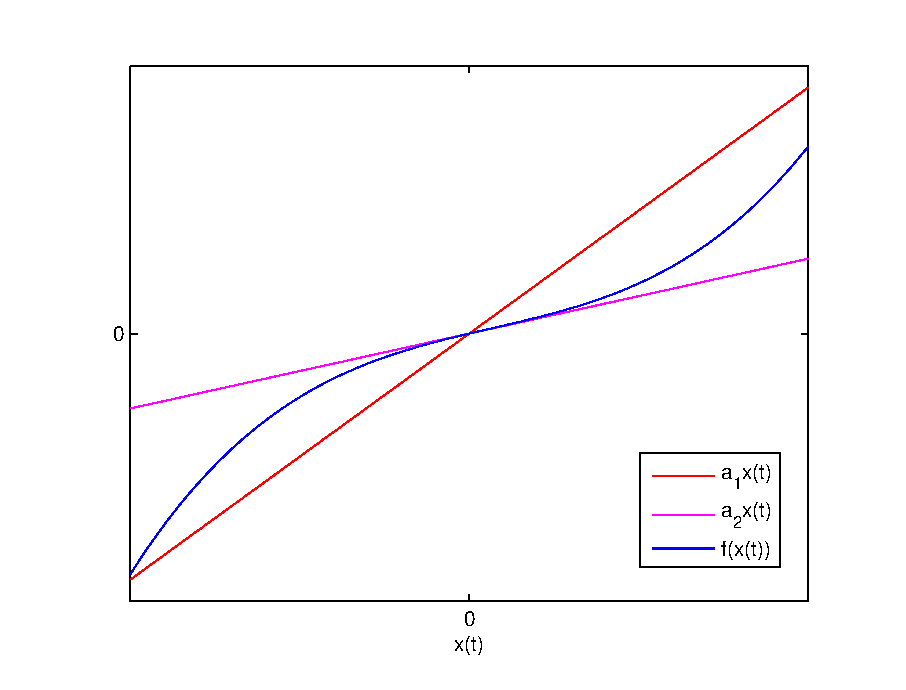
\includegraphics[width=10cm]{global_sector_nonlinearity}
	\caption{Setor global para um dado $f(x(t))$. As curvas em vermelho e em rosa correspondem às retas que limitam o setor global e a curva em azul equivale à função $f(x(t))$.}
	 \label{fig:setor_global}
\end{figure}

Nem sempre, porém, é possível prever o comportamento da função para quaisquer valores de $x(t)$, impossibilitando de se obter um setor global para a modelagem fuzzy Takagi-Sugeno exata do sistema. Assim, para sanar este problema, obtém-se o setor local, que consiste em um setor obtido da mesma forma que o setor global, porém limitado para valores pré-definidos de $x(t)$. A partir daí só se é possível garantir a exatidão do modelo dentro da região contida pelos limites de $x(t)$. Utilizam-se as restrições físicas das varáveis de estado do sistema como limitantes que definem a região do setor local. A Figura \ref{fig:setor_local} mostra a representação de um setor local, limitado por $-d \leq x(t) \leq d$.

\begin{figure}[htbp]
	\centering
	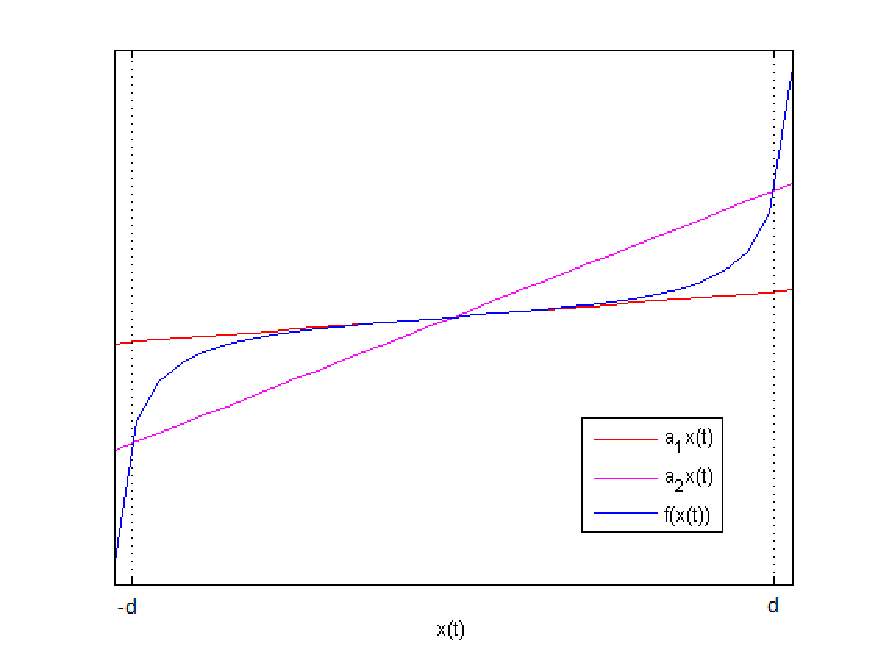
\includegraphics[width=10cm]{local_sector}
	\caption{Setor local para um dado $f(x(t))$. As curvas em vermelho e em rosa correspondem às retas que limitam o setor local e a curva em azul equivale à função $f(x(t))$. As linhas correspondentes aos limites de $x(t)$ estão representadas em preto pontilhado.}
	 \label{fig:setor_local}
\end{figure}

Assim, a modelagem fuzzy Takagi-Sugeno por não linearidade de setor local modela o sistema não linear de forma exata na região contida na configuração poliédrica $\chi$ definida em termos dos k vértices formados por todas as combinações dos limitantes das variáveis de estado, conforme segue.
\begin{equation}\label{eq:rep_poliedrica_por_vertices}
\mathbf{\chi} = co\{x^1, x^2, ... , x^k\}
\end{equation}

Como cada vértice $x^i, i = 1, 2, ..., k$, corresponde a uma combinação diferente entre cada um dos limites superiores e inferiores das variável de estado do sistema, então a região possuirá  $2^n$ vértices. Assim, se um sistema possui três variáveis de estado, por exemplo, haverá 8 vértices delimitando a região poliédrica que contém o ponto de equilíbrio e dentro da qual o sistema será modelado.

 Deste modo, para um sistema com duas variáveis de estado $x_1$ e $x_2$, por exemplo, tal que $-1 \leq x_1 \leq 1 $ e $-2 \leq x_2 \leq 2$, a modelagem por não linearidade de setor local permite obter um modelo válido dentro de uma região poliédrica descrita por quatro vértices resultantes das combinações dos pontos que limitam $x_1$ e $x_2$, os quais são $x^1 = (-1, -2), x^2 = (-1, 2), x^3 = (1, -2), x^4 = (1, 2)$. Esta região pode ser representada graficamente, conforme a Figura \ref{fig:poliedro_exemplo}.

\begin{figure}[htbp]
	\centering
	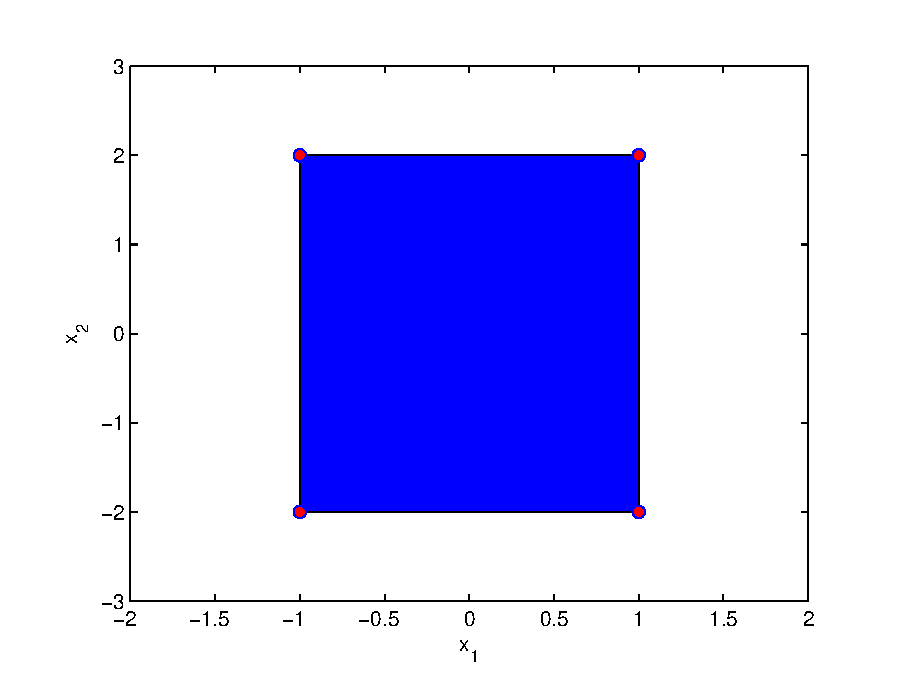
\includegraphics[width=10cm]{polyhedral_set_example}
	\caption{Região poliédrica $\chi$ de um sistema com variáveis de estado limitadas $-1 \leq x_1 \leq 1 $ e $-2 \leq x_2 \leq 2$, em que $\chi$ está representado em azul e os vértices correspondem aos pontos em vermelho.}
	 \label{fig:poliedro_exemplo}
\end{figure}

O modelo fuzzy Takagi-Sugeno obtido a partir do método de não linearidade por setor local apresenta, considerando um modelo não linear com a origem como ponto de equilíbrio, tal qual apresentado na equação \ref{eq:nonlinear_system_without_u}, a seguinte configuração
\begin{equation}\label{eq:fuzzyTS_system}
\mathbf{\dot{x}} = \mathbf{A(\alpha) x}
\end{equation}

Portanto, o objetivo desta o modelagem é obter $\mathbf{A(\alpha)}$, em que
\begin{equation}\label{eq:A_alpha}
\mathbf{A(\alpha)} = \sum_{i=1}^{r} \alpha_i(z) A_i,\qquad\alpha\in\Lambda_r
\end{equation}
Tal que
\begin{equation}\label{lambda_r}
\Lambda_r = \{\alpha \in \rm I\!R^r | \sum_{i = 1}^{r} \alpha_i(z) = 1,\quad \alpha_i(z) \geq 0\}
\end{equation}
De forma que $\alpha_i$ equivale à i-ésima função de associação e $A_i$ ao i-ésimo vértice do sistema, dados os limitantes físicos das variáveis de estado, e r é o número de regras fuzzy. O conjunto $\alpha_i$ das funções de associação é conhecido como primeiro simplex. Os parágrafos seguintes visam apresentar como se obter as funções de associação e os vértices do modelo fuzzy em estudo fazendo-se uso de um exemplo.

A partir a região $\chi$ de interesse e do sistema não linear o qual se pretende obter o modelo fuzzy Takagi-Sugeno, é preciso primeiramente identificar os termos não lineares do sistema, que corresponderão às variáveis de premissa $z_i(x(t)), i = 1, ..., n$ \footnote{A partir deste ponto o argumento t será omitido, para fins de simplificação da notação}. Assim, consideremos o exemplo a seguir retirado da \cite{articlets:2009}, que consiste em um sistema não linear simples que servirá como guia para o entendimento dos métodos de obtenção das fun\c{o}\~ {o}es de pertinência e dos vétices do modelo fuzzy.

\begin{example}
\begin{equation}\label{eq:ex_sal09}
 \begin{bmatrix}\dot{x_1}\\ \dot{x_2} \end{bmatrix} = \begin{bmatrix}0&1 \\-\sin(x_1^2)&0\end{bmatrix}\begin{bmatrix}x_1 \\x_2\end{bmatrix}, \chi = \{(x_1, x_2) | |x_1| \leq 0.5\}
\end{equation}\label{ex:sal09}
\end{example}

\'{E} possível verificar que há apenas uma variável de premissa, $z_1(x) = \sin(x_1^2)$. Conhecendo-se $\chi$, obtêm-se os limites superiores e inferiores de $z_1(x)$, os quais são, respectivamente, $min(z_1(x)) = z_1(0) = 0$ e $max(z_1(x)) = z_1(0.5) = 0.2474$. A não linearidade pode ser expressa, seguindo a metodologia de modelagem por não linearidade por setor local, com uma interpolação entre 0 e 0.2484 dependente do estado $x_1$, conforme a Figura \ref{fig:setor_local_ex_sal09}.
\begin{figure}[htbp]
	\centering
	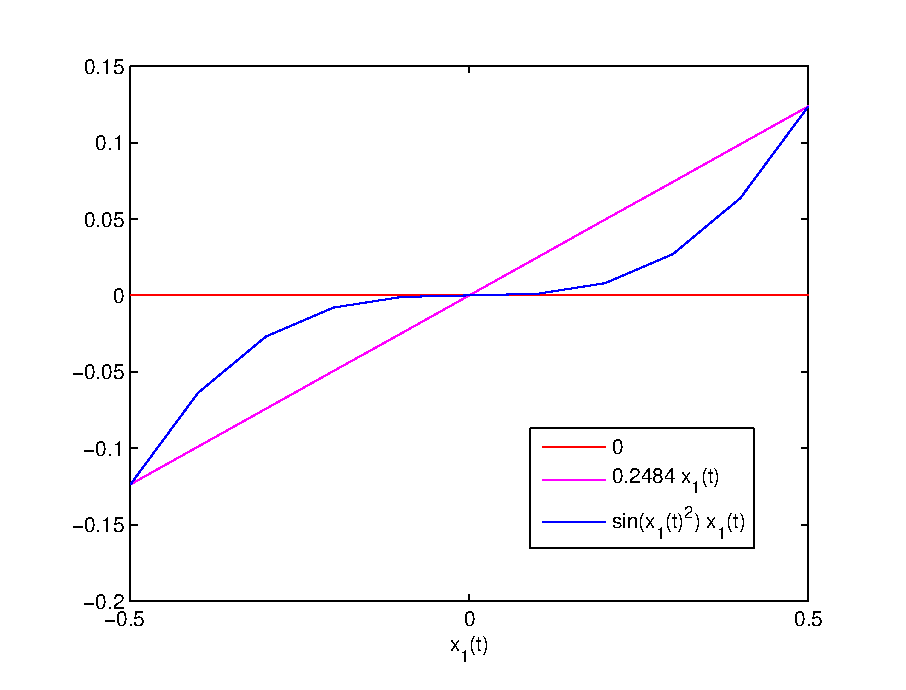
\includegraphics[width=10cm]{local_sector_ex_sal09}
	\caption{Setor local para a não linearidade $z_1 = \sin(x_1^2)$. A curva em vermelho corresponde ao limite inferior da não linearidade, a curva em rosa corresponde ao limite superior e a curva em azul equivale à própria  $z_1$}
	 \label{fig:setor_local_ex_sal09}
\end{figure}

Identificadas as variáveis de premissa e seus valores limites, estas podem ser representadas como \cite{booktw:2003}
\begin{equation}\label{eq:var_premissas_por_grau_pert}
z_i(\textbf{x}) = M_{i1}[z_i(\textbf{x})] \cdot min(z_i(\textbf{x})) + M_{i2}[z_i(\textbf{x})] \cdot max(z_i(\textbf{x})),	\qquad i = 1, .., n
\end{equation}

De forma que $M_{i1}[z_i(x)]$ e $M_{i2}[z_i(\textbf{x})]$ são os grau de associação, ou graus de pertinência, da variável de premissa $z_i(\textbf{x})$. Em outras palavras, $M_{i1}[z_i(\textbf{x})]$ expressa o quanto o limitante superior está associado ao valor assumido por $z_i(\textbf{x})$ para cada valor de \textbf{x} e $M_{i2}[z_i(\textbf{x})]$ expressa o quanto o seu limitante inferior está associado ao valor assumido por $z_i(\textbf{x})$ para cada valor de \textbf{x}. Portanto, deve-se restringir os graus de pertinência para que  sempre seja válida a relação \cite{booktw:2003}
\begin{equation}\label{eq:grau_pert_igual_1}
M_{i1}[z_i(\textbf{x})] + M_{i2}[z_i(\textbf{x})] = 1
\end{equation}

Além disso, $M_{ij}$ devem sempre estar contidos no intervalo [0, 1]. Quando o grau de associação for zero para algum valor de \textbf{x}, implica que $z_i(\textbf{x})$ é corresponde a exatamente o valor do limitante oposto ao deste grau de associação para este valor de \textbf{x}.

Por isso, os graus de associação podem ser calculados conforme mostra a equação \ref{eq:membership_degrees} \cite{booktw:2003}.
\begin{equation}\label{eq:membership_degrees}
M_{i1}[z_i(\textbf{x})] =\dfrac{z_i(\textbf{x})-min(z_i(\textbf{x}))}{max(z_i(\textbf{x}))-min(z_i(\textbf{x}))}, \quad M_{i2}[z_i(\textbf{x})] = 1 - M_{i1} =\dfrac{max(z_i(\textbf{x}))-z_i(\textbf{x})}{max(z_i(\textbf{x}))-min(z_i(\textbf{x}))} 
\end{equation}

Retomando o exempto da equação (\ref{eq:ex_sal09}), obtemos o graus de associação de $z_1(\textbf{x})$, com base no que fora descrito acima. Assim,
\begin{equation}\label{eq:membership_degrees_ex_sal09}
M_{11}[z_1(\textbf{x})] =\dfrac{\sin(x_1^2)}{\sin(0.5^2)}, \quad M_{12}[z_1(\textbf{x})] = 1 - M_{11} =\dfrac{\sin(0.5^2) - \sin(x_1^2)}{\sin(0.5^2)}
\end{equation}

A Figura \ref{fig:setor_local_ex_sal09} mostra as curvas dos graus de associação do sistema para os diferentes valores de $x_1(t)$.

\begin{figure}[htbp]
	\centering
	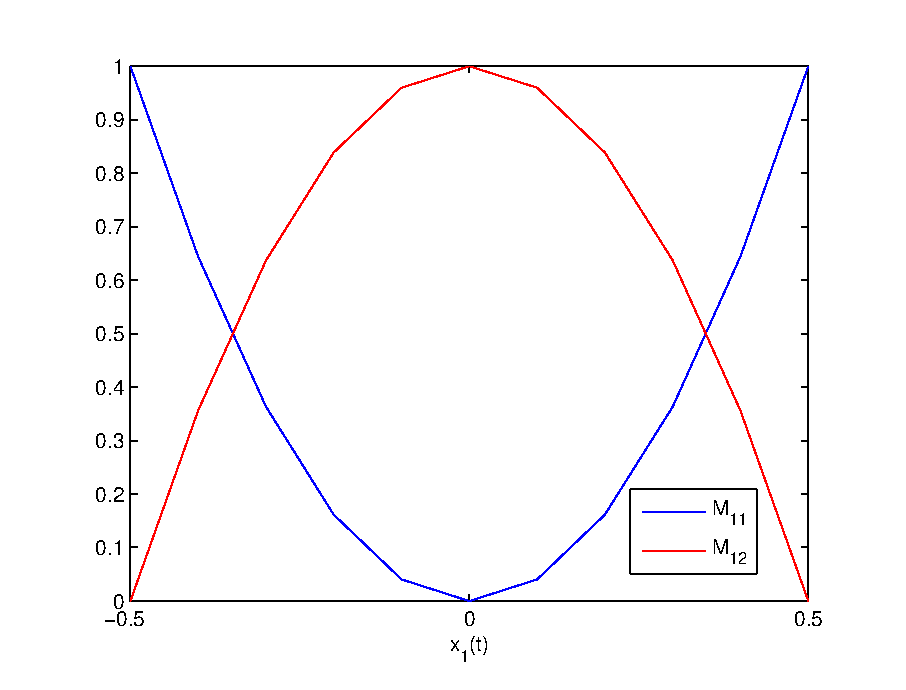
\includegraphics[width=10cm]{membershio_degrees_ex_sal09}
	\caption{Graus de pertinência de $z_1(\textbf{x})$ para o Exemplo \ref{ex:sal09}. A curva em azul corresponde a $M_{11}$ e a curva em vermelho corresponde a$M_{12}$}
	 \label{fig:setor_local_ex_sal09}
\end{figure}

As funções de associação ${\alpha[z(\textbf{x})]}$, por sua vez, relacionam os graus de pertinência das variáveis de premissa para obter o modelo de associação completo do sistema. Portanto, as funções de pertinência são obtidas conforme segue
\begin{equation}\label{eq:membership_functions}
\alpha_i (z)=\prod_{i_1 = 1}^{2} ... \prod_{i_n = 1}^{2} M_{1i_1}... M_{ni_n}
\end{equation}

Para o Exemplo \ref{ex:sal09}, como há apenas uma variável de premissa, as funções de associação equivalem aos graus de associação. Logo,
\begin{equation}\label{eq:membership_functions_ex_sal09}
\alpha_1(z) = \dfrac{\sin(x_1^2)}{\sin(0.5^2)}, \quad \alpha_2(z) = \dfrac{\sin(0.5^2) - \sin(x_1^2)}{\sin(0.5^2)}
\end{equation}

Por último, para se obter os vértices $\textbf{A}_i$ do modelo fuzzy Takagi-Sugeno, basta substituir todas variáveis de premissa $z_i(\textbf{x})$ na matriz $\textbf{A}$ do sistema não linear por cada uma das combinações  possíveis de seus valores máximos e mínimos \footnote{As combinações dos limitantes das variáveis de premissa em \textbf{A(x)} podem ser obtidas seguindo o modelo de representação binária sem sinal. Em que se assume que cada valor, iniciado por zero e indo até $2^n-1$, é representado por $n$ dígitos, sendo o primeiro correspondente a $z_1(\textbf{x})$ e o n-ésimo correspondente a $z_n(\textbf{x})$. Assim, quando o primeiro digito for 0 (zero),  $z_1(\textbf{x}) = min(z_1(\textbf{x}))$. Quando for 1 (um), $z_1(\textbf{x}) = max(z_1(\textbf{x}))$, e assim sucessivamente.}.

No exemplo que vimos nesta seção, os vértices são
\begin{equation*}
\textbf{A}_1 (\textbf{z}) =
 \begin{bmatrix}0&1 \\-min(z_1)&0\end{bmatrix} = 
\begin{bmatrix}0&1 \\-\sin(0)&0\end{bmatrix} = 
\begin{bmatrix}0&1 \\0&0\end{bmatrix}
\end{equation*}
\begin{equation*}
\textbf{A}_2(\textbf{z})= \begin{bmatrix}0&1 \\-max(z_1)&0\end{bmatrix} = \begin{bmatrix}0&1 \\-\sin(0.5^2)&0\end{bmatrix} = \begin{bmatrix}0&1 \\-0.2474&0\end{bmatrix}
\end{equation*}

\subsection{Algoritmo para obtenção do modelo fuzzy Takagi-Sugeno}

Com base no que fora dito até agora, é possível obter o modelo fuzzy Takagi-Sugeno para um setor local para qualquer sistema não linear seguindo os passos listados a seguir, tendo em mente que o sistema defuzificado será no formato

\begin{equation}\label{eq:modelo_fuzzy_TS}
\mathbf{\dot{x}} =\sum_{i=1}^{r}\alpha_i(z( \mathbf{x})) \mathbf{A_ix}
\end{equation}

\begin{enumerate}
\item Dado um sistema de equações não lineares com entradas forçadas nulas, representá-lo na forma matricial, tal que
\begin{equation*}
\mathbf{\dot{x}} = \mathbf{A(x)x}
\end{equation*}
\item Identificar as variáveis de premissa $z_1, ... z_n$, onde cada uma equivale a uma não linearidade distinta em \textbf{A(x)} dependente de  \textbf{x}.
\item Obter a quantidade de regras $r$ do modelo, a partir da quantidade $n$ de variáveis de premissa obtidas no item anterior, conforme segue.
\begin{equation*}
r = 2^n
\end{equation*}
\item A partir das limitações físicas das variáveis de estado do sistema, ou seja, a partir dos limites de valores que cada variável de estado pode assumir, definir os valores máximo, $max(z_i)$, e mínimo, $min(z_i)$, de cada variável de premissa.
\item Obter os graus de pertinência $M_{ij}$ do modelo para cada variável de premissa, conforme a Equação (\ref{eq:membership_degrees}).
\item Obter as $r$ funções de pertinência, conforme Equação (\ref{eq:membership_functions}).
\item Obter os $r$ vértices $\mathbf{A_i}$ do modelo, a partir da aplicação de todas as $2^n$ combinações possíveis dos valores máximos e mínimos das variáveis de premissa na matriz \textbf{A(x)} do modelo não linear.
\item Finalmente, utilizar os dados obtidos nos itens anteriores para montar o modelo defuzzificado da Equação (\ref{eq:modelo_fuzzy_TS}).
\end{enumerate}

\subsection{Exemplos}

Nesta seção serão apresentadas as modelagens fuzzy Takagi-Sugeno dos três exemplos apresentados na seção \ref{subsection:descr_exemplos}.

\begin{example}[Sistema não linear de segunda ordem \cite{article:LPJ:2011}]\end{example}\label{ex:LPJ12_fuzzyTS}
O exemplo \ref{example_LPJ12} consiste em um sistema de segunda ordem de dinâmica não linear, descrito conforme Equação (\ref{eq:LPJ12_dinamica}), em que $x_1$ é limitado por $-\pi/2 \leq x_1 \leq pi/2$

\begin{equation}\label{eq:LPJ12_dinamica}
\begin{bmatrix}\dot{x_1}\\ \dot{x_2} \end{bmatrix} = \begin{bmatrix} -2 & 4\\  -1 - \dfrac{\lambda (1 - sen(x_1))}{2} & -2 \end{bmatrix} \begin{bmatrix}x_1 \\ x_2 \end{bmatrix}
\end{equation}

Nota-se que o sistema possui apenas um termo não linear, ou seja, possui apenas uma variável de premissa $z_1 = sen(x_1(t))$. Conhecendo-se os limitantes da variável de estado $x_1$, obtemos os limitantes de $z_1$. Assim,

\begin{equation*}max(z_1(x(t))) = 1\quad min(z_1(x(t))) = -1\end{equation*}

Assim, obtém-se as funções de pertinência e os vértices do modelo fuzzy Takagi-Sugeno deste sistema, que são apresentados no Exemplo 2 da referência bibliográfica \cite{article:LPJ:2011}, conforme segue.
\begin{equation*}
\alpha_1(z(t)) = \dfrac{1+\sin(x_1(t))}{2}\qquad \alpha_2(z(t)) = 1 - h_1(z(t))
\end{equation*}
\begin{equation*}
A_1 = \begin{bmatrix}-2&4\\-1&-2\end{bmatrix}\qquad A_2 = \begin{bmatrix}-2&4\\-(1+\lambda)&-2\end{bmatrix}
\end{equation*}

O sistema não linear e o sistema fuzzy Takagi-Sugeno foram simulados e as curvas das respostas plotadas, conforme mostra a Figura \ref{fig:sim_fuzyy_TS_ex2_LPJ12}. Escolheu-se arbitrariamente o ponto inicial $\begin{bmatrix}x_{{inicial}_1}&x_{{inicial}_2}\end{bmatrix}' = \begin{bmatrix}-\pi/3&\pi/3\end{bmatrix}'$.

\begin{figure}[htbp]
	\centering
	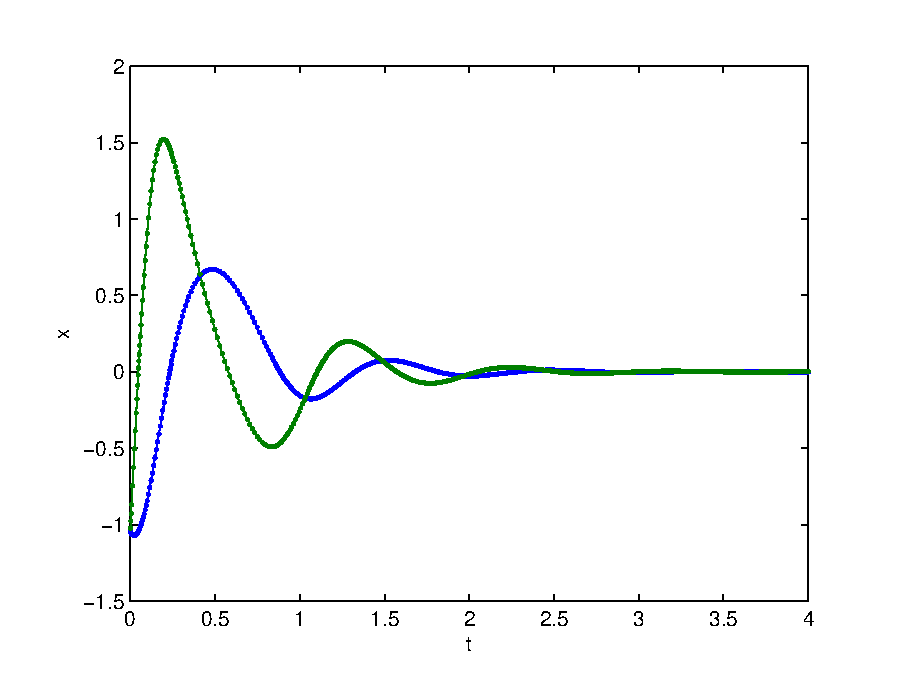
\includegraphics[width=10cm]{fuzzy_TS_sim_ex2_LPJ12}
	\caption{Respostas $x_1$ e $x_2$ do modelo não linear e do modelo fuzyy Takagi-Sugeno para o sistema de segunda ordem \cite{article:LPJ:2011}. As curvas em azul equivalem a $x_1$ e as curvas em verde a $x_2$. O modelo não linear corresponde às linhas contínuas, enquanto o modelo fuzzy T-S corresponde ás linhas pontilhadas}
	 \label{fig:sim_fuzyy_TS_ex2_LPJ12}
\end{figure}

As curvas obtidas da simulação dos modelos não linear e fuzzy T-S do exemplo \ref{ex:LPJ12_fuzzyTS} permitem verificar que estes modelos são completamente correspondentes entre si.

\begin{example}[Sitema droop]\label{ex:droop_UFSM_fuzzyTS}

Considerando o Exemplo \ref{ex:droop_UFSM}, que consiste no modelo Droop do inversor, as equações do sistema não linear com o ponto de equilíbrio na origem podem ser apresentadas na forma matricial, conforme segue.

\begin{equation}\label{eq:sist_droop_UFSM_mat}
\begin{bmatrix}\dot{x_{d_1}}\\\dot{x_2}\\\dot{x_3}\end{bmatrix} =\begin{bmatrix}-\omega_f - \dfrac{-\omega_fVn}{R_o}\cos(x_3)&0&\frac{\varphi(x_3)}{x_3}\\
\dfrac{\omega_fVn}{R_o}\sin(x_3)&-\omega_f&-\dfrac{\omega_fV(E_{ref}-n(x_1^*-P_{ref}))}{R_o}\dfrac{\sin(x_3)}{x_3}\\
0&m&0\end{bmatrix}\begin{bmatrix}x_{d_1}\\x_2\\x_3\end{bmatrix}
\end{equation}
onde $\varphi(x_3) = \dfrac{\omega_f}{R_o}(V(E_{ref}-n(x_1^* - P_{ref}))\cos(x_3) - V^2) - \omega_fx_1^*$.
\end{example}

O sistema possui quatro variáveis de premissa
\begin{equation*}
  \begin{gathered}
z_1 = \cos(x_3)\\
z_2 = \dfrac{\varphi(x_3)}{x_3}\\
z_3 = \sin(x_3)\\
z_4 = \dfrac{sin(x_3)}{x_3}
\end{gathered}
\end{equation*}

Desta maneira, a matriz $A(x)$ da equação \ref{eq:sist_droop_UFSM_mat} pode ser reescrita em função das variáveis de premissa.
\begin{equation}\label{eq:A_z}
A(z) = \begin{bmatrix}-\omega_f - \dfrac{-\omega_fVn}{R_o}z_1&0&z_2\\
\dfrac{\omega_fVn}{R_o}z_3&-\omega_f&-\dfrac{\omega_fV(E_{ref}-n(x_1^*-P_{ref}))}{R_o}z_4\\
0&m&0\end{bmatrix}
\end{equation}

Os limites máximo e mínimo das variáveis de premissa são obtidos levando em consideração os limites físicos de $x_3$, os quais só permitem valores contidos na região $\begin{bmatrix}-0.02&0.1\end{bmatrix}$. Assim, os limites superiores e inferiores de $\textbf{z}$ são obtidos, conforme as seguintes relações.
\begin{equation*}
\begin{gathered}
z_{1_{min}} = min(\cos(x_3)) \qquad  z_{4_{max}} = max(\cos(x_3))\\
z_{2_{min}} = min(\dfrac{\varphi(x_3)}{x_3}) \qquad  z_{2_{max}} = min(\dfrac{\varphi(x_3)}{x_3})\\
z_{3_{min}} = min(\sin(x_3)) \qquad  z_{3_{max}} = max(\sin(x_3))\\
z_{4_{min}} = min(\dfrac{sin(x_3)}{x_3}) \qquad z_{4_{max}} = max(\dfrac{sin(x_3)}{x_3})
\end{gathered}
\end{equation*}

O ponto $x_3 = 0$ não deve ser considerado para a obtenção dos limitantes de $\textbf{z}$ para que sejam evitadas indeterminações. Como foram identificadas quatro variáveis de premissa a partir do modelo não linear, o modelo fuzzy possuirá dezesseis vértices, os quais são representados pelas matrizes $A_i, i = 1, ... ,16$, em função das diferentes combinações de$ z_{j_{min}}$ e $z_{j_{max}}, j = 1, ..., 4$, conforme descrito abaixo.
\begin{equation}\label{eq:A_fuzzy_4_vertices}
\begin{gathered}
A_1 = A(z_{1_{min}}, z_{2_{min}}, z_{3_{min}}, z_{4_{min}})\\
A_2 = A(z_{1_{min}}, z_{2_{min}}, z_{3_{min}}, z_{4_{max}})\\
A_3 = A(z_{1_{min}}, z_{2_{min}}, z_{3_{max}}, z_{4_{min}})\\
A_4 = A(z_{1_{min}}, z_{2_{min}}, z_{3_{max}}, z_{4_{max}})\\
A_5 = A(z_{1_{min}}, z_{2_{max}}, z_{3_{min}}, z_{4_{min}})\\
A_6 = A(z_{1_{min}}, z_{2_{max}}, z_{3_{min}}, z_{4_{max}})\\
A_7 = A(z_{1_{min}}, z_{2_{max}}, z_{3_{max}}, z_{4_{min}})\\
A_8 = A(z_{1_{min}}, z_{2_{max}}, z_{3_{max}}, z_{4_{max}})\\
A_9 = A(z_{1_{max}}, z_{2_{min}}, z_{3_{min}}, z_{4_{min}})\\
A_{10} = A(z_{1_{max}}, z_{2_{min}}, z_{3_{min}}, z_{4_{max}})\\
A_{11} = A(z_{1_{max}}, z_{2_{min}}, z_{3_{max}}, z_{4_{min}})\\
A_{12} = A(z_{1_{max}}, z_{2_{min}}, z_{3_{max}}, z_{4_{max}})\\
A_{13} = A(z_{1_{max}}, z_{2_{max}}, z_{3_{min}}, z_{4_{min}})\\
A_{14} = A(z_{1_{max}}, z_{2_{max}}, z_{3_{min}}, z_{4_{max}})\\
A_{15} = A(z_{1_{max}}, z_{2_{max}}, z_{3_{max}}, z_{4_{min}})\\
A_{16} = A(z_{1_{max}}, z_{2_{max}}, z_{3_{max}}, z_{4_{max}})\\
\end{gathered}
\end{equation}

Cada variável de premissa possui dois graus de associação, concordante com a equação \ref{eq:membership_degrees}. Já as funções de associação são obtidas a partir da equação \ref{eq:membership_functions}.

Finalmente, conhecendo-se os valores numéricos dos parâmetros do sistema, obtém-se o modelo fuzzy Takagi-Sugeno do sistema droop. Tanto o modelo não linear quanto o modelo fuzzy T-S deste sistema foram simulados para o valor inicial igual a $\begin{bmatrix}10000&1000&0.01\end{bmatrix}$, o qual está dentro do hiperplano $C$ delimitado pelos valores máximos e mínimos que cada variável de estado pode assumir. As curvas obtidas da simulação foram plotadas e são apresentadas na Figura \ref{fig:sim_fuzyy_TS_droop_UFSM}, lembrando que $x_1 = P_f$, $x_2 = Q_f$ e $x_3 = \delta$.

\begin{figure}[htbp]
	\centering
	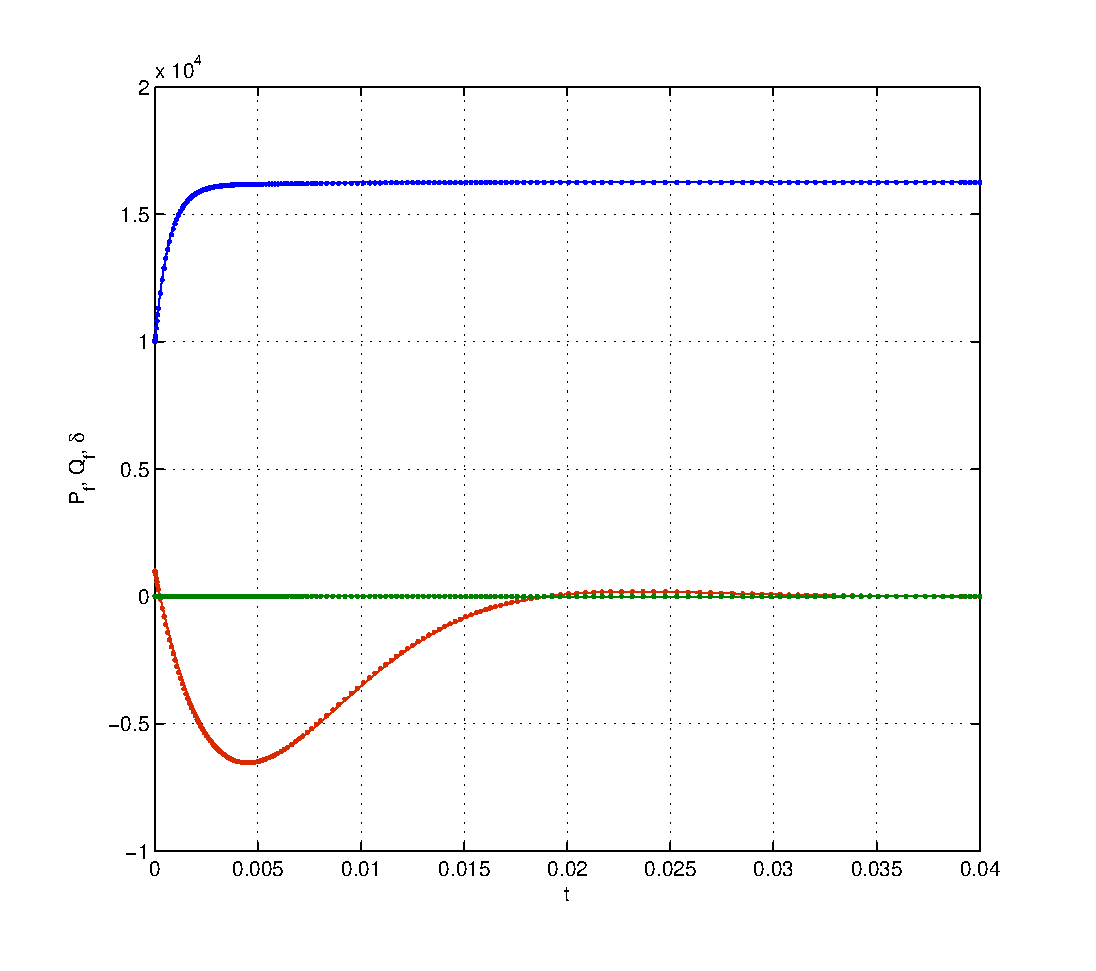
\includegraphics[width=10cm]{fuzzy_TS_sim_droop_UFSM}
	\caption{Respostas $P_f$, $Q_f$ e $\delta$ do modelo não linear e do modelo fuzzy Takagi-Sugeno para o sistema de droop com $\textbf{x}_{inicial} = [10000\quad1000\quad0]'$. As curvas em azul equivalem a $P_f$, as curvas em verde a $\delta$ e em vermelho, $Q_f$. O modelo não linear corresponde às linhas contínuas, enquanto o modelo fuzzy T-S corresponde às linhas pontilhadas}\label{fig:sim_fuzyy_TS_droop_UFSM}
\end{figure}

A Figura \ref{fig:sim_fuzyy_TS_droop_UFSM} evidencia que o modelo fuzzy T-S obtido corresponde a exatamente o modelo não linear do sistema.

Para verificar o comportamento dos estados fora do setor local delimitado por $C$, foi escolhido arbitrariamente um ponto $\textbf{x}_{inicial}$ fora desta região. O ponto escolhido foi $\textbf{x}_{inicial} = \begin{bmatrix}1000000&-100000&0.3\end{bmatrix}$' e as respostas do modelo não linear e do modelo fuzzy T-S são apresentadas na Figura \ref{fig:fuzzy_droop_out} e na Figura \ref{fig:sim_fuzzy_TS_droop_UFSM_out_of_C}.

\begin{figure}[htbp]
	\centering
	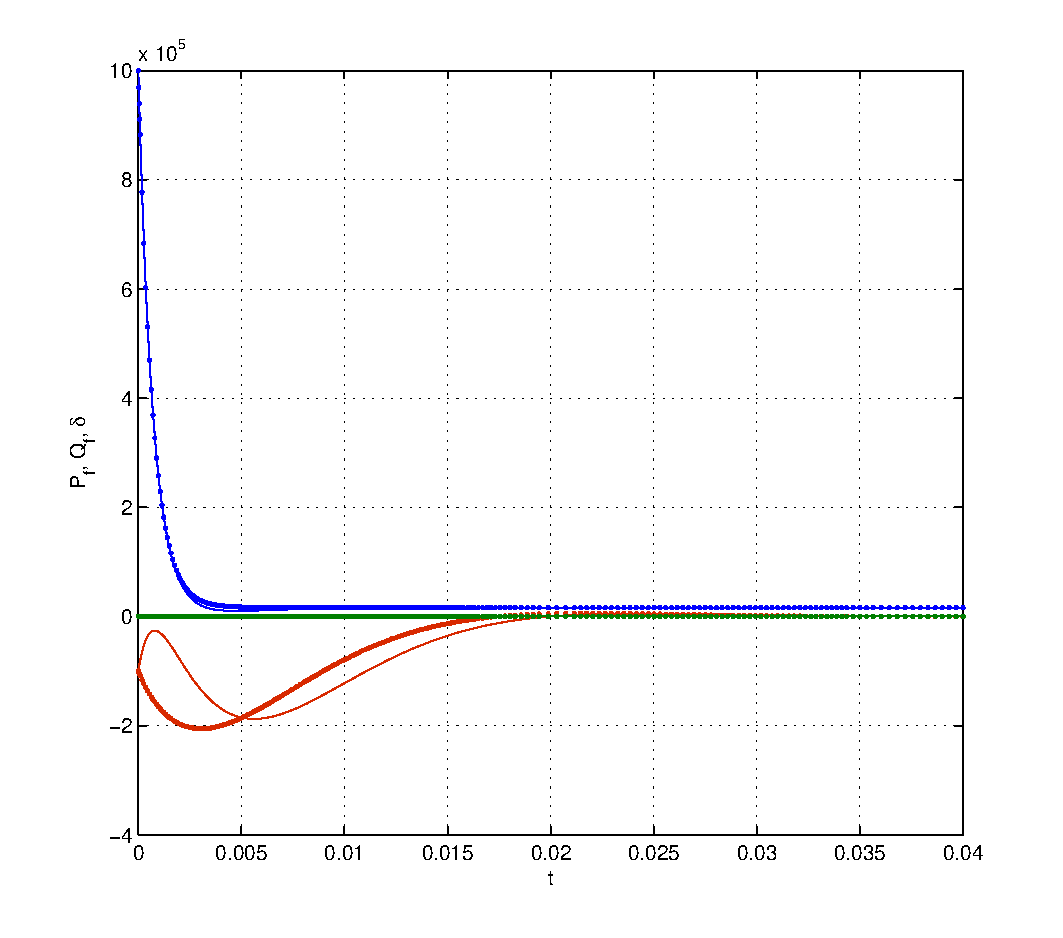
\includegraphics[width=10cm]{fuzzy_TS_sim_droop_UFSM_out_of_C}
	\caption{Respostas $P_f$, $Q_f$ e $\delta$ do modelo não linear e do modelo fuzyy Takagi-Sugeno para o sistema de droop com $\textbf{x}_{inicial} = [1000000\quad-100000\quad0.3]'$ fora da região $C$. As curvas em azul equivalem a $P_f$, as curvas em verde a $\delta$ e em vermelho, $Q_f$. O modelo não linear corresponde às linhas contínuas, enquanto o modelo fuzzy T-S corresponde às linhas pontilhadas}\label{fig:sim_fuzzy_TS_droop_UFSM_out_of_C}
\end{figure}

\begin{figure}[htbp]
	\centering
	\subfigure[ref1][$P_f$]{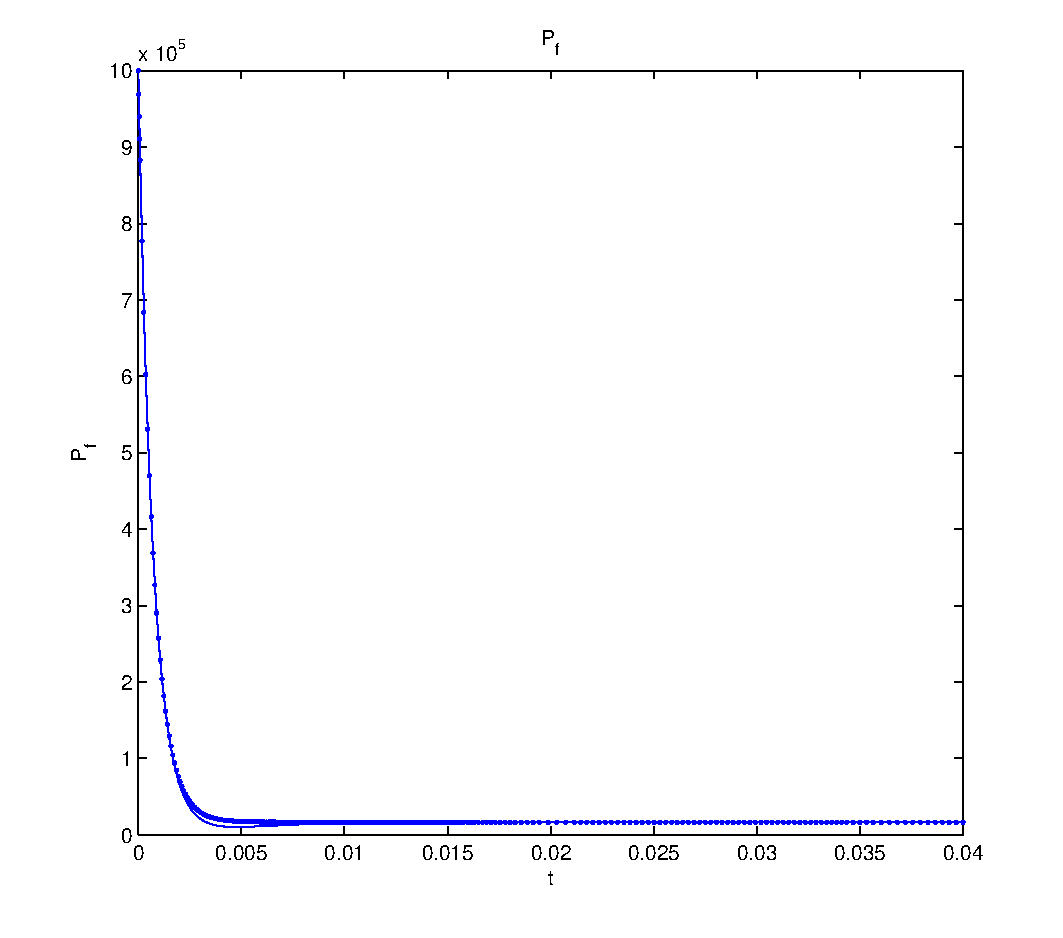
\includegraphics[width=7cm]{P_f_out_of_C}}
	\qquad
	\subfigure[ref2][$Q_f$]{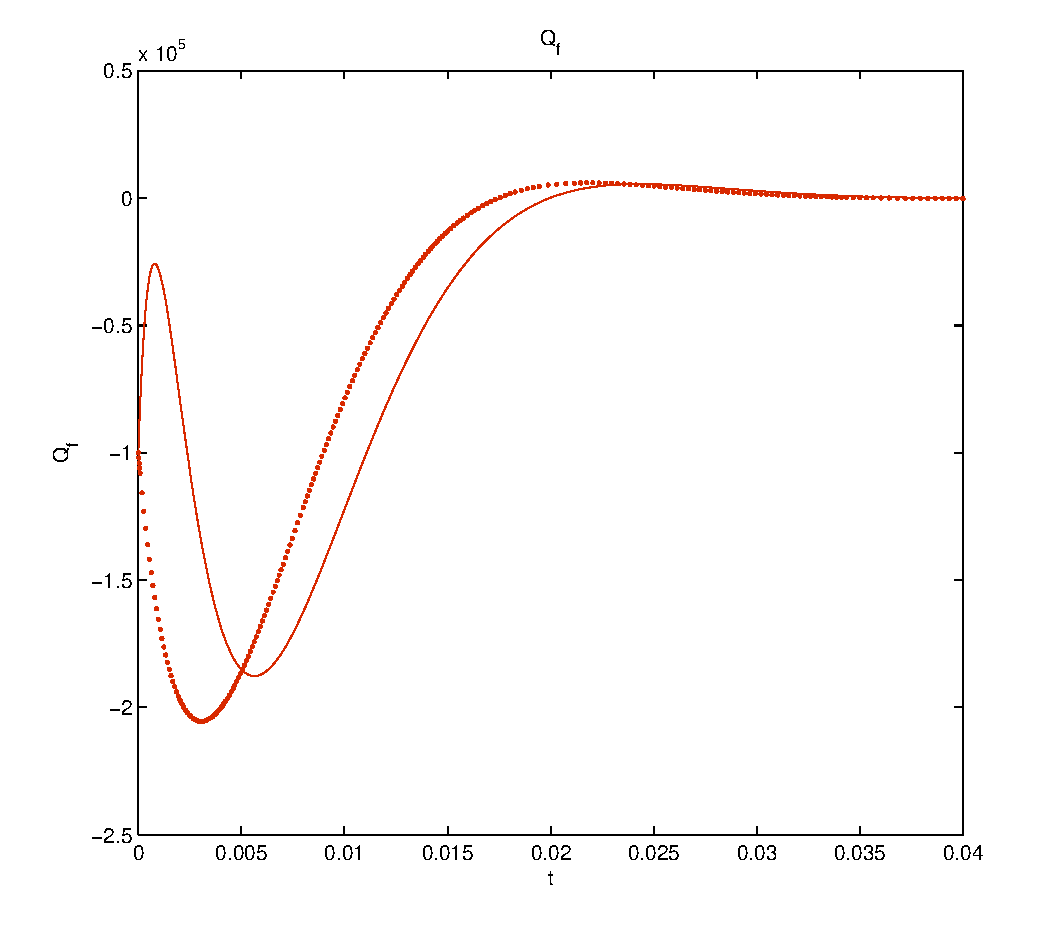
\includegraphics[width=7cm]{Q_f_out_of_C}}
	\qquad
	\subfigure[ref3][$\delta$]{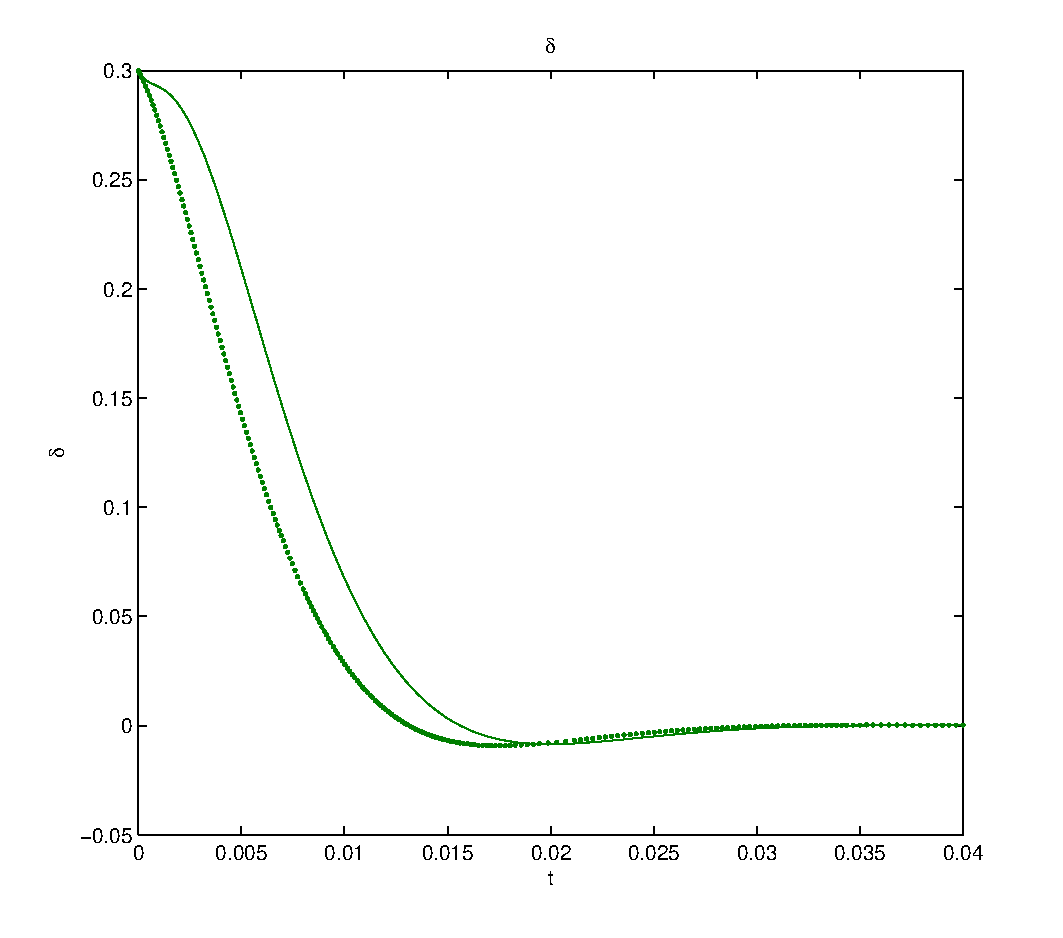
\includegraphics[width=7cm]{delta_out_of_C}}
	\caption{Resposta do sistema droop para o ponto inicial $\textbf{x}_{inicial} = [1000000\quad-100000\quad0.3]'$ fora da região $C$ em função do tempo. Em linha contínua são representadas as respostas dos modelo nã-linear e em pontilhado as respostas do modelo fuzzy}
	\label{fig:fuzzy_droop_out}
\end{figure}

A partir das Figuras \ref{fig:fuzzy_droop_out} e \ref{fig:sim_fuzzy_TS_droop_UFSM_out_of_C} é possível notar que o modelo fuzzy T-S não é válido fora da região C, para qual se obteve este modelo. Este conclusão é verificada pelo fato de que o modelo fuzzy T-S não corresponde ao modelo não linear para o ponto inicial fora de C.

\begin{example}[Processo de quatro tanques]\label{ex:4_tanques} O exemplo \ref{example_4tanques} apresenta um sistema que utiliza duas bombas para controlar o nível de água dentro de dois tanques inferiores. Cada uma das bombas, além de abastecer um dos tanques inferiores, também abastece um dos tanques superiores, os quais, por sua vez, despejam seus conteúdos nos tanques inferiores. O modelo não linear deste sistema é apresentado na forma matricial na Equação (\ref{eq:4tanques_matrix}). Além disso, devido ás limitações físicas da planta, foi assumido que as variáveis de estado $h_1$, $h_2$, $h_3$ e $h_4$ do sistema somente assumirão valores contidos no intervalo $[0, 23 cm]$.
\end{example}

A partir do modelo não linear, é possível verificar que o sistema possui quatro não linearidades, que serão equivalentes às variáveis de premissa do sistema, as quais são
\begin{equation*}
z_1 = \dfrac{\sqrt{(h_1)}}{h_1}\quad z_2 = \dfrac{\sqrt{(h_2)}}{h_2}\quad z_3 = \dfrac{\sqrt{(h_3)}}{h_3}\quad z_4 = \dfrac{\sqrt{(h_4)}}{h_4}
\end{equation*}

Os valores máximos $z_{i_{max}}$ e mínimos $z_{i_{min}}$ das variáveis de premissa são obtidos desconsiderando o ponto $h_i = 0$, para que não ocorra a indeterminação de divisão por zero. Desta maneira, obtiveram-se  $z_{i_{max}} = 3.1623$ e $z_{i_{min}} = 0.2085, i = 1, 2, 3, 4$.

Por ter quatro variáveis de premissa, o sistema possui dezesseis vértices. A matriz $\textbf{A(x)}$ do modelo não linear do processo pode ser reescrita em função das variáveis de premissa, conforme mostra a Equação (\ref{eq:A_z_fuzzy_4_tqs}).
\begin{equation}\label{eq:A_z_fuzzy_4_tqs}
\textbf{A(z)} =\begin{bmatrix}-\dfrac{a_1}{A_1}\cdot \sqrt{2\cdot g}\cdot z_1&0
&\dfrac{a_3}{A_1}\cdot \sqrt{2\cdot g}\cdot z_3&0
\\0&-\dfrac{a_2}{A_2}\cdot \sqrt{2\cdot g }\cdot z_2
&0&\dfrac{a_4}{A_2}\cdot \sqrt{2\cdot g}\cdot z_4
\\0&0&-\dfrac{a_3}{A_3}\cdot \sqrt{2\cdot g}\cdot z_3&0
\\0&0&0&-\dfrac{a_4}{A_4}\cdot \sqrt{2\cdot g }\cdot z_4\end{bmatrix}
\end{equation}

Os vértices de 16 $\textbf{A(z)}$ são obtidos a partir de todas as combinações possíveis entre dos valores máximos e mínimos das variáveis de premissa, conforme já apresentado na Equação (\ref{eq:A_fuzzy_4_vertices}).

Cada variável de premissa possui dois graus de associação, que são obtidos a partir da Equação (\ref{eq:membership_degrees}). As funções de associação, por sua vez, são obtidas a partir da Equação (\ref{eq:membership_functions}).

A matriz $B$, associada às entradas do sistema, também compõe os vértices do sistema. Porém, como $B$ não depende dos estados, continua no modelo fuzzy exatamente como é para o modelo não linear, de forma que os 16 vértices $B_i, i = 1, 2,\hdots, 16$ serão iguais a $B$.

Neste exemplo, o modelo defuzzyficado aparece na forma
\begin{equation}\label{eq:fuzzyTS_system_with_B}
\mathbf{\dot{x}} = \mathbf{A(\alpha)x+Bu}
\end{equation}
Que pode ser reescrita como
\begin{equation}\label{eq:A_alpha_B}
\mathbf{\dot{x}} = \sum_{i=1}^{r} \alpha_i(z) A_ix + Bu
\end{equation}

O modelo não linear e do modelo fuzzy Takagi-Sugeno do processo de quatro tanques foram simulados e as curvas de resposta foram obtidas, conforme mostra a Figura \ref{fig:4_tanques_sim_TS}. Embora o sistema tenha como limitação a altura máxima igual a $23 cm$ para o nível de água em cada um dos tanques, estas alturas não foram saturadas nas simulações. Isto foi feito para que se pudesse verificar a não exatidão do modelo fora da região da modelagem fuzzy Takagi-Sugeno.
\begin{figure}[htbp]
	\centering
	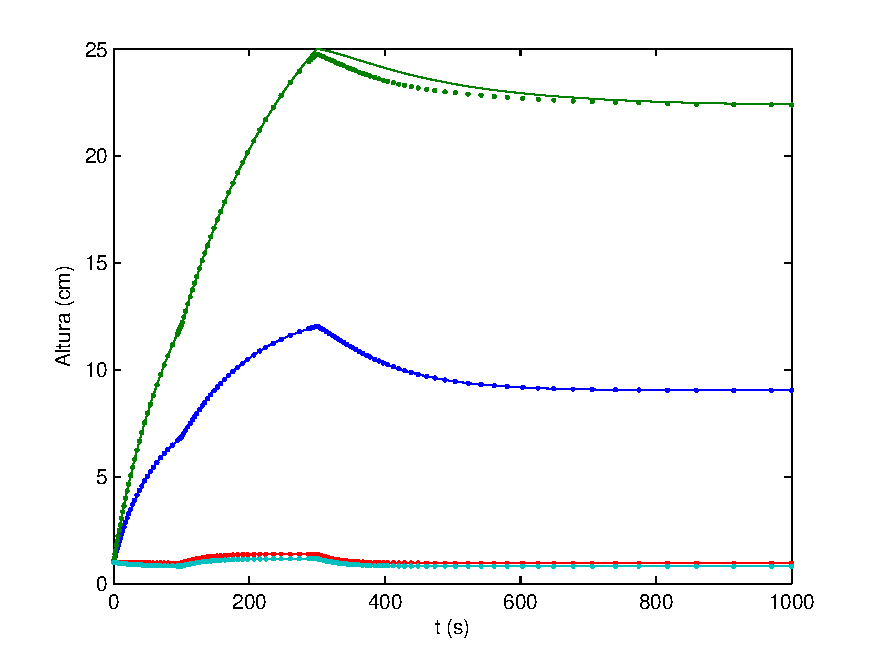
\includegraphics[width=10cm]{4_tanks_simulation}
	\caption{Respostas $h_1$, $h_2$, $h_3$ e $h_4$ do modelo não linear e do modelo fuzyy Takagi-Sugeno para o processo de quatro tanques com $\textbf{h}_{inicial} = [8.9\quad9.97\quad8.65\quad9.67]'$ e entradas $\upsilon = [1\quad1]$. As curvas em azul equivalem a $h_1$, em verde tem-se $h_2$, em vermelho, $h_3$, e em azul claro $h_4$. O modelo não linear corresponde às linhas contínuas, enquanto o modelo fuzzy T-S corresponde às linhas pontilhadas}\label{fig:4_tanques_sim_TS}
\end{figure}

A simulação do processo de quatro tanques permite concluir que a modelagem fuzzy Takagi-Sugeno modela de forma exata o sistema não linear dentro da região para a qual a modelo foi definido, ou seja, dentro do setor local. Em contrapartida, quando os estados se afastam da região para a qual o modelo fuzzy T-S foi definido, como é o caso de $h_1$, que ultrapassa a altura de $23 cm$ na simulação, é possível notar que o modelo deixa de ser exato.

\section{Considerações Finais}\label{sec:consid_finais}
Neste capítulo foi apresentado o conceito de retrato de fase para resposta de sistemas. O retrato de fase é utilizado para verificar de forma qualitativa a estabilidade do ponto de equilíbrio de sistemas não lineares, uma vez que estes têm um comportamento difícil de se prever, justamente devido aos termos não lineares que contêm. Vimos que quando as respostas se aproximam do ponto de equilíbrio à medida que o tempo passa, este é dito como estável. Por outro lado, quando as respostas se afastam do ponto de equilíbrio com o passar do tempo, diz-se que este ponto de equilíbrio é instável. Também foram vistos outros tipos de conclusões que podem ser verificadas a respeito da estabilidade de pontos de equilíbrio.
Os principais exemplos utilizados para aplicação dos conceitos discutidos neste trabalho também foram apresentados nesta seção. Por último, mas não menos importante, foi apresentada a técnica de modelagem por lógica fuzzy, proposta por Takagi e Sugeno \cite{articlets:1985} para a obtenção de um modelo constituído por um conjunto de representações linearizadas do sistema não linear. Este modelo garante a exatidão, quando comparado com o sistema não linear, dentro de uma região definida no plano de estados.

Para se obter o sistema fuzzy Takagi-Sugeno exato para uma região definida no espaço de estados, utilizou-se o artifício de modelagem por não linearidade de setor, proposto por Tanaka e Wang \cite{booktw:2003}. Os modelos fuzzy Takagi-Sugeno foram obtidos para cada um dos exemplos propostos e foi possível verificar a exatidão desta modelagem em relação ao modelo não linear para a região definida na obtenção do modelo. O contrário também foi observado quando para pontos fora da região para a qual o sistema fuzzy T-S foi obtido.

Nos próximos capítulos serão apresentadas técnicas para a análise de estabilidade de pontos de equilíbrio de sistemas utilizando o modelo fuzzy Takagi-Sugeno e função de Lyapunov, assim como técnicas para a obtenção do domínio de atração destes pontos de equilíbrio, quando estáveis. Os resultados obtidos neste capítulo serão utilizados tanto para obtenção das funções de Lyapunov para verificação da estabilidade, a partir do modelo fuzzy T-S, quanto para verificação de validade dos domínios de atração dos pontos de equilíbrio estável por meio de comparações com os respectivos retratos de fase.

% *** Estabilidade de Sistemas não lineares ***
\chapter{Estabilidade de Sistemas Não Lineares}\label{cap_EstSistNaoLin}


\section{Introdução}

A estabilidade é o desempenho mínimo de todo sistema de controle, por isso é a primeira propriedade a ser verificada antes que se inicie o projeto do controlador para este sistema. Neste trabalho, mais especificamente neste capítulo, nos despenderemos em determinar a estabilidade de pontos de equilíbrio de sistemas não lineares. O método a ser utilizado para a determinação da estabilidade dos pontos de equilíbrio dos sistemas em estudo consiste na chamada Estabilidade de Lyapunov, proposta em 1892  pelo matemático e engenheiro russo que dá nome a esta teoria \cite{bookkhalil:2003}. A teoria de Estabilidade de Lyapunov investiga o comportamento da resposta do sistema em torno do ponto de equilíbrio situado na origem do plano de estados, de forma tal que permite não apenas determinar se o ponto de equilíbrio é estável, assintoticamente estável ou instável, mas, caso se conclua que o ponto de equilíbrio equivale a uma dentre as duas primeiras possibilidades supracitadas, permite também obter a estimativa da região no plano de estados para a qual a estabilidade do ponto é valida. A região para a qual o ponto de equilíbrio é um ponto estável ou assintoticamente estável é dita região de atração do ponto de equilíbrio, a qual será objeto de estudo do capítulo \ref{cap_RegAtrac}. Neste capítulo, portanto, vamos nos ater a verificar a estabilidade para o ponto de equilíbrio do sistema situado na origem do plano de estados segundo proposto por Lyapunov.

\section{Estabilidade de Lyapunov}

Antes de definir Estabilidade de Lyapunov, mais especificamente Estabilidade de Lyapunov via LMIs, que será a abordagem utilizada neste trabalho, será feita uma breve contextualização de como se dá o uso de funções de Lyapunov para o estudo de estabilidade de um ponto de equilíbrio na origem. Para tanto, será utilizado o exemplo do pêndulo simples.

\subsection{Estabilidade de um ponto de equilíbrio}

Antes de definirmos de forma sistemática a estabilidade de Lyapunov, vamos retomar uma discussão iniciada no Capítulo \ref{cap_ModelagemSisNaoLinearesporFuzzyTS}. Na Seção \ref{subsec_phasePortrait} vimos que um ponto de equilíbrio é caracterizado conforme o comportamento da resposta do sistema a partir de pontos iniciais próximos a este. Se as respostas permanecem próximas ao ponto de equilíbrio, este é dito estável, caso contrário, é instável. O ponto de equilíbrio é assintoticamente estável se, quando o tempo tende ao infinito, a resposta do sistema tende ao ponto de equilíbrio.

Considerando um sistema não linear autônomo, ou seja, independente do tempo, constituído de equações de estado não forçadas descrito por

\begin{equation}\label{sist_autonomo}
\mathbf{\dot{x} = f(x)}
\end{equation}

Onde o domínio de $\textbf{f}$ é tal que $\textbf{f}: C \rightarrow I\!R^n$, com $C \subset I\!R^n$, tal que $\textbf{0} \in D$. Supondo também que $\textbf{x = 0}$ sempre será o ponto de equilíbrio do sistema da equação \ref{sist_autonomo}, a definição de estabilidade de um ponto de equilíbrio pode ser reescrita, segundo descrito por \cite{bookkhalil:2003}, conforme apresentado a seguir.

\begin{defn} (Khalil, 2003)\cite{bookkhalil:2003}\label{def:pontoEquilibrio}
 O ponto de equilíbrio \textbf{x = 0} de \ref{sist_autonomo} é
\begin{itemize}
\item estável se, para cada $\varepsilon > 0$, existe $\delta = \delta(\varepsilon) > 0$ tal que
\begin{equation*} ||\textbf{x}(0)|| < \delta \Rightarrow ||\textbf{x}(t)|| < \varepsilon, \forall t \geq 0
\end{equation*}
\item instável, se não for estável;
\item assintoticamente estável se for estável e $\delta$ puder ser escolhido tal que
\begin{equation*}||\textbf{x}|| <\delta \Rightarrow \lim_{x\to\infty} \textbf{x}(t) = 0
\end{equation*}
\end{itemize}
 \end{defn}

Em outras palavras, a Definição \ref{def:pontoEquilibrio} diz que, para qualquer valor de $\varepsilon$ escolhido, tem-se um valor de $\delta = \delta(\varepsilon)$ tal que uma trajetória começando em uma vizinhança $\delta$ da origem nunca deixará a vizinhança $\varepsilon$. A Figura \ref{fig:epsilon_delta} exemplifica esta definição. A região delimitada pela linha azul contendo a origem equivale a $\delta$, esta região contém todas as possibilidades de pontos iniciais tais que as respostas do sistema jamais deixem a região $\varepsilon$ contendo a origem, representada pela cor vermelha na figura.

\begin{figure}[htbp]
	\centering
	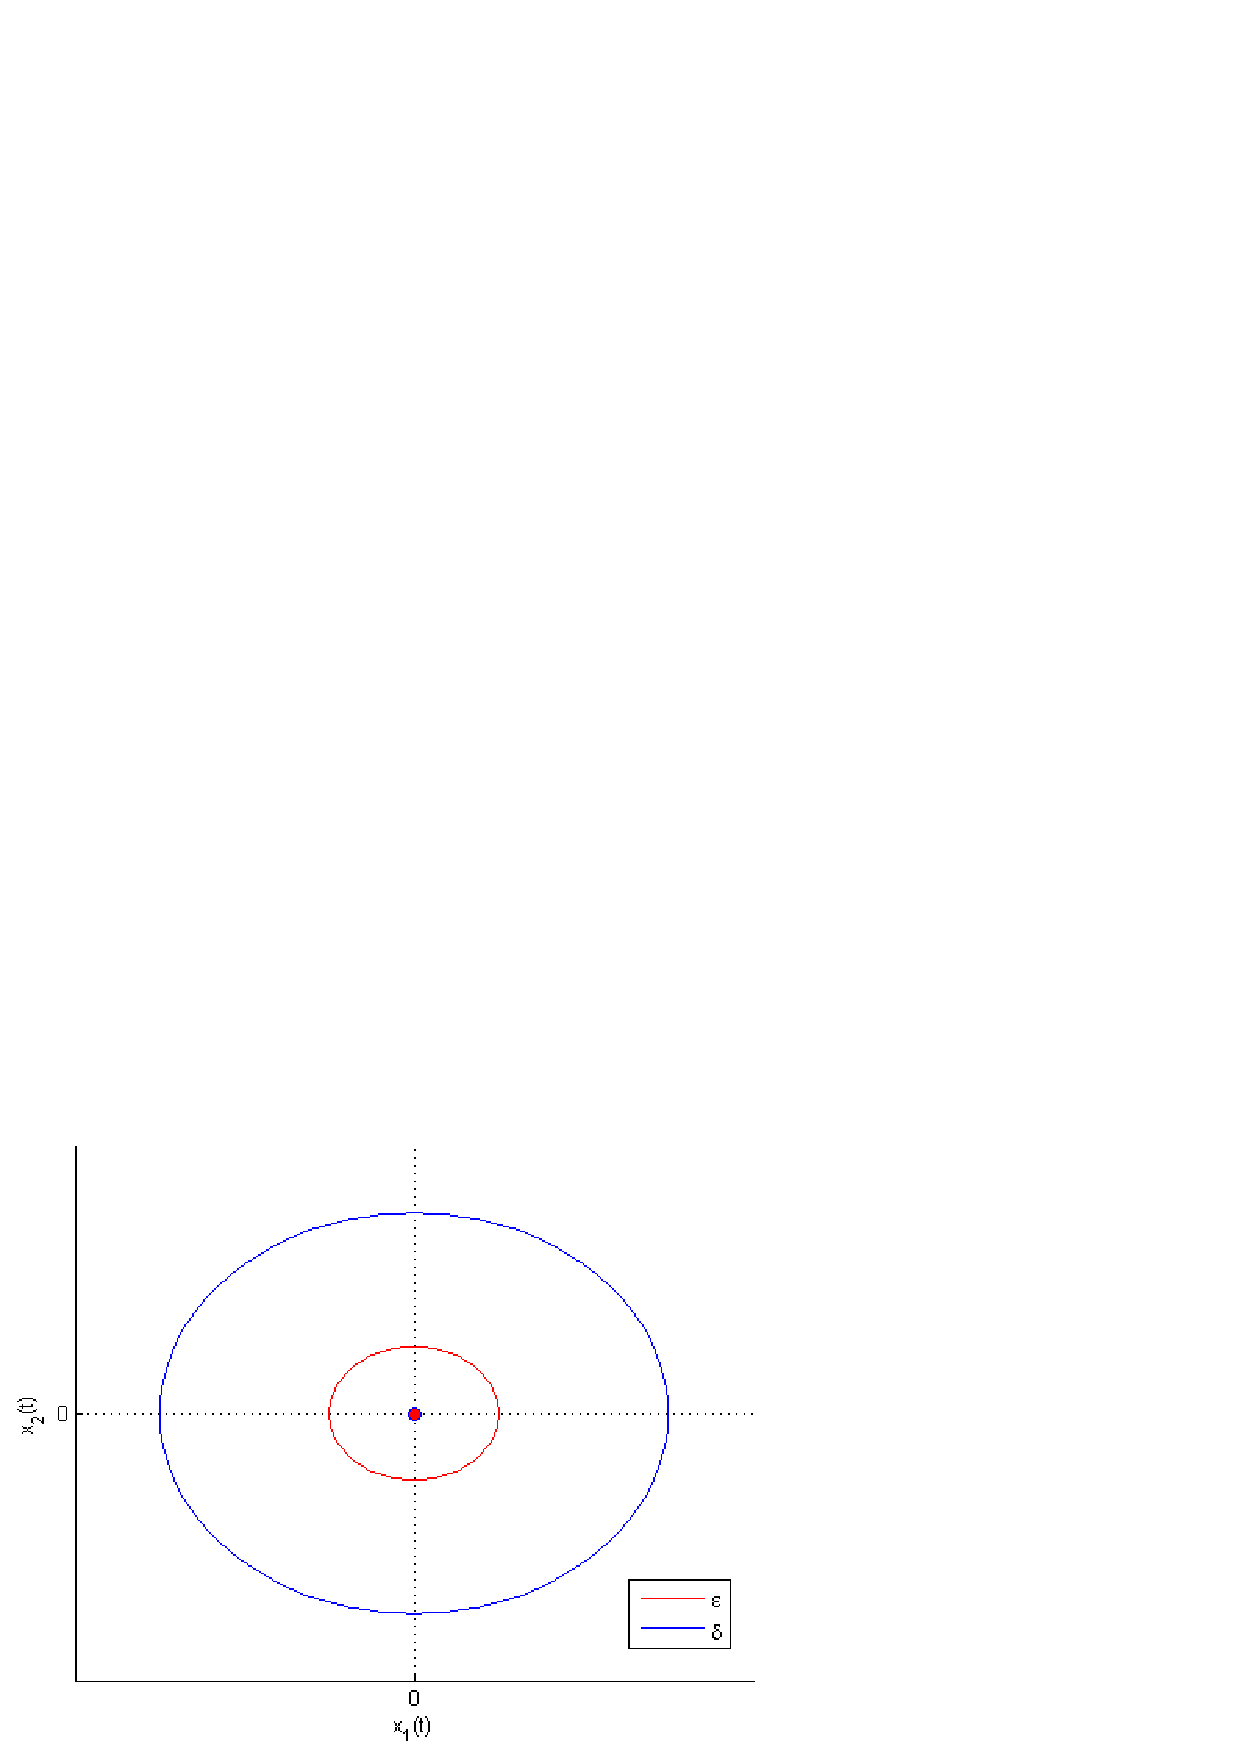
\includegraphics[width=10cm]{epsilon_delta}
	\caption{Região $\varepsilon$, em vermelho, e $\delta$, em azul, utilizadas para definir a estabilidade do ponto de equilíbrio na origem}
	 \label{fig:epsilon_delta}
\end{figure}

Vale lembrar, que, como visto no capítulo anterior, caso o ponto de equilíbrio do sistema não seja na origem, este pode ser deslocado para a origem sem que haja perda de generalidade. Para tanto, basta utilizar o método de mudança de variável.

Para ilustrar as properiedades de estabilidade de um ponto de equilíbrio segundo a Definicção \ref{def:pontoEquilibrio}, será analisado o modelo de um pêdulo \cite{bookkhalil:2003}, o qual é é descrito no exemplo a seguir.

\begin{example} [Pêndulo simples] Considere o pêndulo simples mostrado na Figura \ref{fig:pendulo}, onde $L$ é o comprimento da haste e $m$ é a massa do prumo na ponta da haste. Assuma que a haste é rígida e que tem massa igual a zero e que o pêndulo é livre de balanço no plano vertical. $\theta$ é o ângulo entre a haste e o eixo vertical. A haste do pêndulo se move num círculo de raio L. 

\begin{figure}[htbp]
	\centering
	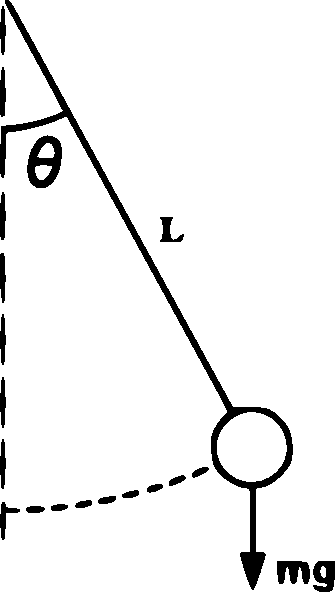
\includegraphics[width=4cm, height=6cm]{pendulum}
	\caption{Pêndulo simples}
	 \label{fig:pendulo}
\end{figure}

A equação de movimento do pêndulo pode ser obtida utilizando-se a segunda lei de Newton, considerando que há uma componente de força gravitacional igual a $mg$ agindo sobre o prumo, onde $g$ é a aceleração da gravidade. Além disso, há um componente de atrito $k$, que é proporcional \`{a} valocidade do prumo. Assim obtém-se a equação de movimento na direção tangencial, conforme segue.
\begin{equation*} mL\ddot{\theta} = -mg\sin\theta - kL\dot{theta}
\end{equation*}
Assumindo $x_1 = \theta$ e $x_2 = \dot{\theta}$, o modelo de estados do pêndulo passa a ser
\begin{equation*}
\begin{cases}\dot{x_1} = x_2\\\dot{x_1} = -\dfrac{g}{L} \sin(x_1) - \dfrac{k}{m} x_2
\end{cases}
\end{equation*}

Os pontos de equilíbrio do pêndulo simples são obtidos fazendo-se $\dot{x_1} = \dot{x_2} = 0$ e resolvendo para $x_1$ e $x_2$. Logo, os pontos de equilíbrio são $(x_1,x_2) = (0,0)$ e $(x_1, x_2) = (\pi,0)$. O retrato de fase do sistema para valores arbitrários dos parâmetros é mostrado na Figura \ref{fig:pendulo_retrato_fase}, onde a Figura (a) equivale ao retrato de fase considerando-se o atrito diferente de zero e a Figura (b) assume atrito igual a zero.

\begin{figure}[htbp]
	\centering
	\subfigure[ref1][Retrato de fase considerando atrito diferente de zero]{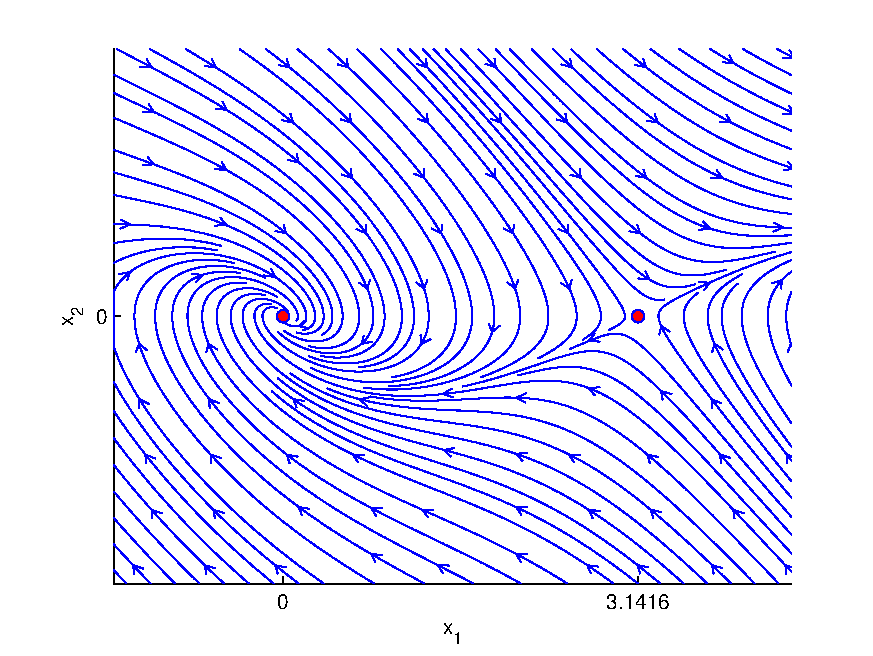
\includegraphics[width=7cm]{pendulum_phase_portrait}}
	\qquad
	\subfigure[ref2][Retrato de fase considerando atrito igual a zero]{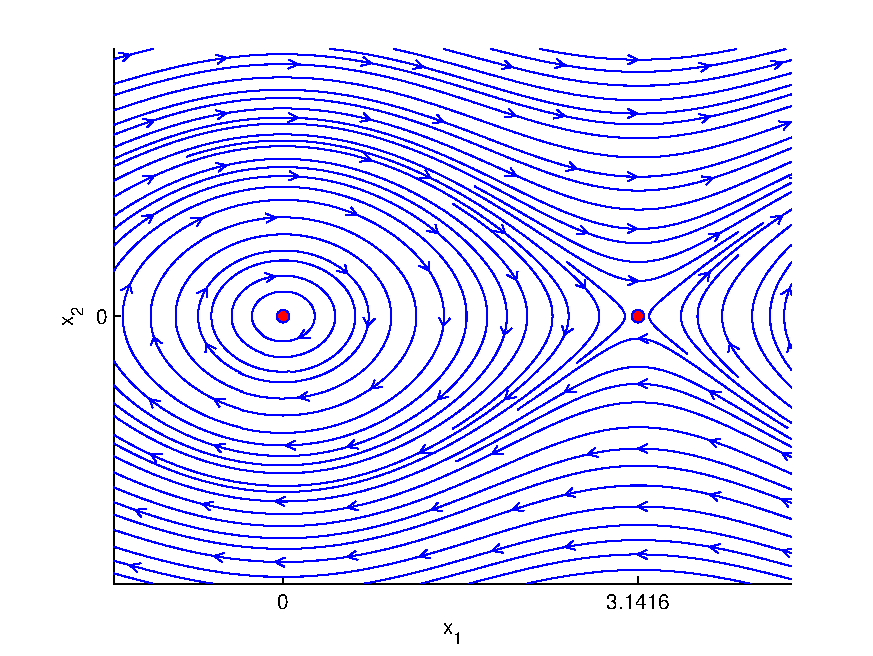
\includegraphics[width=7cm]{pendulum_phase_portrait_k_0}}
	\caption{Retrato de fase do pêndulo simples com atrito diferente de zero e com atrito igual a zero}
	\label{fig:pendulo_retrato_fase}
\end{figure}

\end{example}\label{ex:pendulo_simples}

Neste exemplo do pêndulo simples, quando o atrito é nulo, as trajetórias na vizinhança do ponto de equilíbrio $(0,0)$ são órbitas fechadas. Assim, escolhendo-se um ponto inicial suficientemente perto deste ponto de equilíbrio, é garantido que as trajetórias permanecerão sempre em torno deste, de forma que a relação $\varepsilon-\delta$ necessária para a estabilidade é satisfeita.

No caso em que o atrito é considerado, o ponto de equilíbrio localizado na origem, além de as trajetórias na vizinhança manterem-se próximas a este, estas também tendem ao ponto de equilíbrio quando o tempo tende ao infinito. Mais uma vez, verifica-se que  a origem do plano de estados e sua vizinhança satisfaz a relação $\varepsilon-\delta$ necessária para a estabilidade e, desta vez, também verifica-se que este ponto é assintoticamente estável. Já o ponto de equilíbrio $(\pi, 0)$ se comporta como um ponto de sela e, em ambos os caso, em que se assume o atrito diferente de zero e, em seguida, igual a zero, não se é possível obter uma região $\delta$ tal que as respostas estejam sempre contidas em uma região $\varepsilon$, pois sempre haverá uma trajetória que sairá desta região.

A verificação da estabilidade de pontos de equilíbrio por meio do retrato de fase é uma técnica bastante limitada, pois somente pode ser aplicada para sistemas de, no máximo, terceira ordem. E, ainda, tem-se a desvantagem de ser difícil de se observar o comportamento das trajetórias de resposta ao redor do ponto de equilíbrio para sistemas de terceira ordem, como visto no exemplo \ref{ex:droop_UFSM}.

Como uma tentativa de se obter de forma generalizada e objetiva conclusões sobre a estabilidade dos pontos de equilíbrio do sistema, pode-se utilizar conceitos de energia \cite{bookkhalil:2003}. Neste exemplo, portanto, considera-se que a energia total do sistema é obtida da soma da energia potencial e da energia cinética, com a referência da energia potencial escolhida como sendo zero quando as variáveis de estado são iguais a zero. Para o atrito nulo, não há dissipação de energia, logo, a energia total do sistema é constante durante o movimento, ou seja, a variação de energia é igual a zero ao longo das trajetórias do sistema ($dE/dt = 0$). O fato de a energia total $E$ ser constante mesmo com o passar do tempo para qualquer valor das variáveis de estado $\textbf{x}$ permite obter uma curva correspondente a um contorno fechado ao redor da origem do plano de estados de raio $r = E$, podendo-se constatar a estabilidade do ponto de equilíbrio $(0,0)$.

Quando se considera a influência do atrito, a variação da energia total $E$ é negativa ($dE/dt \leq 0$), ou seja, a energia se dissipa ao longo tempo. Quando o tempo tende ao infinito, a energia se dissipa totalmente, porém, para cada instante de tempo, a energia total equivale a um valor constante cada vez menor, revelando diferentes contornos que satisfazem a condição para estabilidade, até que o raio da curva tende a zero, revelando que o ponto é assintoticamente estável.

Desta maneira, verifica-se que apenas examinando a variação da energia ao longo das trajetórias do sistema é possível determinar a estabilidade do ponto de equilíbrio. O que Lyapunov propõe em sua teoria de estabilidade é que diversas outras funções, além da energia total do sistema, podem ser usadas, de forma semelhante ao que foi ilustrado acima, para determinar a estabilidade de um ponto de equilíbrio. A próxima seção traz a definição do modelo de determinação de estabilidade proposto por Lyapunov via LMIs.

\subsection{Estabilidade de Lyapunov via Desigualdades Matriciais Lineares (LMIs)}

Antes de iniciar a discussão sobre Estabilidade de Lyapunov nesta seção, será primeiramente introduzido o conceito de função convexa e, em seguida, de Desigualdades Matriciais Lineares (LMIs, do inglês \textit{Linear Matrix Inequalities}), uma vez que as soluções propostas neste trabalho utilizam sistemas convexos e as LMIs são ferramentas poderosas para resolver de forma eficiente este tipo de sistema.

Um conjunto $S$ definido no $\rm I\!R^{n}$ é dito convexo se contém qualquer segmento reta formada a partir de dois pontos quaisquer pertencentes a este conjunto, isto é , $x, y \in S,\quad\lambda,\mu\geq0,\quad\lambda+\mu=1\Rightarrow\lambda x +\mu y\in S$ \cite{inproc:hin:2004}. A Figura \ref{fig:sets_exmples} ilustra um conjunto convexo e de um conjunto não convexo, respectivamente.

\begin{figure}[htbp]
	\centering
	\subfigure[ref1][Conjunto Convexo]{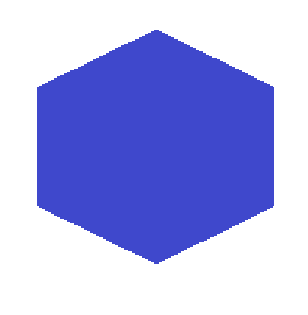
\includegraphics[width=5cm]{convex_set_example}}
	\qquad
	\subfigure[ref2][Conjunto não convexo]{
\includegraphics[width=5cm]{nonconvex_set_example}}
	\caption{Conjuntos convexo e não convexo}
	\label{fig:sets_exmples}
\end{figure}

Uma função $f$ é dita convexa se seu domínio é convexo e para todo $x \in \textbf{dom} f, \theta \in [0, 1]$ vale a seguinte relação.
\begin{equation*}
f(\theta x+(1-\theta)y) \leq f(x)+(1-\theta)f(y)
\end{equation*}

Uma LMI é uma desigualdade matricial do tipo $F(g) > 0$, definida no domínio $\rm I\!R^{m}$ e com imagem em $\rm I\!R^{q \times q}$, simétrica e afim nas variáveis de busca, representadas pelo vetor $g$. Uma representação genérica de uma LMI é dada por
\begin{equation}\label{eq:rep_lmi}
F(g) = F_0+\sum_{i = 1}^{m}g_iF_i>0\quad g = \begin{bmatrix}g_1\\\vdots\\g_m\end{bmatrix}
\end{equation}
em que $F_i = F_i' \in \rm I\!R{q \times q}$ são matrizes dadas e $g_i$ são variáveis escalares a serem determinadas de forma a satisfazer a desigualdade, quando existe uma solução para tal, ou seja, quando a LMI é factível. Dificilmente uma LMI aparecerá na forma gerérica da Equação \ref{eq:rep_lmi}, no entanto, a conversão para este formato é feita internamente pelos pacotes de resolção de LMI aqui utilizados.

Definido o conceito de LMI, estamos agora aptos a discutir sobre a análise de estabilidade proposta por Lyapunov via LMIs. O teorema de estabilidade de Lyapunov caracteriza a estabilidade de um sistema através de uma função $V(x)$, chamada função de Lyapunov, a qual deve satisfazer algumas condições, que serão apresentadas mais a frente. A principal vantagem atrelada ao teorema de Lyapunov é o fato de este poder ser aplicado para determinação da estabilidade de um sistema $\dot{\textbf{x}} = f(\textbf{x})$ sem que se precise resolvê-lo. Por outro lado, não há um método sistemático para se obter funções de Lyapunov, sendo responsabilidade do projetista determiná-las.

Considere $V(x)$ uma função contínua, diferenciável definida no domínio $D \subset \rm I\!R^{n}$, tal que em $D$ esteja contida a origem. A variação de $V(x)$ ao longo das trajetórias do sistema $\dot{x} = f(x)$ é dada por

\begin{equation*}
\dot{V}(x) = \sum_{i = 1}^{n} \frac{\partial V}{\partial x_i}\dot{x}_i = \sum_{i = 1}^{n} \frac{\partial V}{\partial x_i} f_i(x) = \begin{bmatrix}\frac{\partial V}{\partial x_1},&\hdots,&\frac{\partial V}{\partial x_n}\end{bmatrix}\begin{bmatrix}f_1(x)\\\vdots\\f_n(x)\end{bmatrix} = \frac{\partial V}{\partial x}f(x)
\end{equation*}

Logo, $\dot{V}(x)$ é dependente da equação do sistema e, portanto, será diferente para cada sistema \cite{bookkhalil:2003}. E, se $\dot{V}$ for negativa, então $V$ diminui ao longo do tempo da solução do sistema. Assim, o teorema de Lyapunov é enunciado, conforme segue.

\begin{theorem}[Khalil, 2003 \cite{bookkhalil:2003}]\label{th:lyap_stability}
 Seja $x = 0$ um ponto de equilíbrio do sistema não linear autônomo $\dot{x} = f(x)$ e seja $D \subset \rm I\!R^{n}$ um domínio contendo $x = 0$. Seja $V: D \rightarrow \rm I\!R$ uma função diferenciável contínua tal que
\begin{equation}\label{eq:def_V}
V(0) = 0\quad\text{e}\quad V(X) > 0\quad\text{em}\quad D - \{0\}
\end{equation}
\begin{equation}\label{eq:def_dot_V_stable}
\dot{V}(x) \leq 0\quad\text{em}\quad D
\end{equation}
então, $x = 0$ é estável. Além disso, se
\begin{equation}\label{eq:def_dot_V_assymp_stable}
\dot{V}(x) < 0\quad\text{em}\quad D - \{0\}
\end{equation}
então $x = 0$ é assintoticamente estável.
\end{theorem}

As inequações enunciadas no Terorema \ref{th:lyap_stability} são conhecidas como Inequações de Lyapunov. Estas inequações equivalem \`{a}s primeiras LMIs utilizadas para analisar a estabilidade de sistemas dinâmicos, podendo ser resolvidas analiticamente, a partir de um conjunto de equações lineares. As Inequações de Lyapunov são cada vez mais utilizadas  em aplicações em problemas práticos, importantes e difíceis na engenharia de controle.

A função de Lyapunov $V(x)$, utilizada para a determinação da estabilidade de sistemas aparece na forma de funções quadráticas, conhecida como forma quadrática \cite{bookboydl:1994}.

Uma forma quadrática equivale a uma função $\nu(x)$ definida no espaço $\rm I\!R^{n}$ tal que
\begin{equation}\label{eq:forma_quadr}
\nu(x) = \sum_{i = 1}^{n}\sum_{j = 1}^{n}p_{ij}x_ix_j,\quad p_{ij} = p_{ji}
\end{equation}
Em que $x_i$ e $x_j$ são componentes quaisquer do vetor de estados $x$ e $p_{ij}$ são constantes. O exemplo a seguir apresenta uma forma quadrática simples.

\begin{example}\label{ex:forma_quadr}
\begin{equation*}
V(x) = 9x_1^2+3x_1x_2+7x_1x_2+6x_2^2 = 9x_1^2+10x_1x_2+6x_2^2 = 9x_1^2+5x_1x_2+5x_1x_2+6x_2^2
\end{equation*}
\end{example}

É válido também dizer que toda forma quadrática pode ser representada em termos matriciais a partir de uma matriz simétrica cujos elementos são as constantes $p_{ij}$. Assim o Exemplo \ref{ex:forma_quadr} é reescrito na forma
\begin{equation*}
V(x) = \begin{bmatrix}x_1\\x_2\end{bmatrix}'\begin{bmatrix}9&5\\5&6\end{bmatrix}\begin{bmatrix}x_1\\x_2\end{bmatrix} = x'Px
\end{equation*}

Sabendo que toda matriz simétrica possui autovalores reais, a função $\nu(x) = x'Px$ é positiva para todo $x \neq 0$ se, e somente se, os autovalores de $P$ forem todos positivos. Quando satisfeita esta condição, a matriz $P$ é dita positiva definida ($P > 0$) \cite{bookboydl:1994}.

\subsection{Definição do problema}\label{subsec:contextualization}

Considere o sistema não linear
\begin{equation}\label{eq:nonlinear_system_cap_stability}
\dot{\mathbf{x}} = f(\mathbf{x}(t))
\end{equation}
tal que a origem é um ponto de equilíbrio, ou seja, $f(\textbf{0}) = \textbf{0} \in \rm I\!R^p$, em que $p$ é a ordem do sistema, isto é, a quantidade de variáveis de estado. Considere, ainda, a representação fuzzy T-S exata obtida pelo método de aproximação por não linearidade de setor, como visto no capítulo anterior, tal que
\begin{equation}\label{eq:fuzzy_TS_system_cap_stability}
\dot{\mathbf{x}} = A(\mathbf{\alpha) x}(t)
\end{equation}
onde $A(\alpha) \in \rm I\!R^{p \times p}, \forall x(t) \in \chi$, em que $\chi$ é uma região no espaço de estados incluindo a origem, para a qual o sistema está definido. Além disso,
\begin{equation}\label{eq:A_alpha_cap_stability}
A(\alpha) = \sum_{i = 1}^{r} \alpha_i(z)A_i
\end{equation}
Desta maneira, define-se $\alpha(z) = [\alpha_1, ..., \alpha_r] \in \Lambda_r$, em que
\begin{equation}\label{lambda_r}
\Lambda_r = \{\alpha \in \rm I\!R^r | \sum_{i = 1}^{r} \alpha_i(z) = 1,\quad \alpha_i(z) \geq 0\}
\end{equation}
e $z(t)$ são as variáveis de premissa dependentes dos estados, o que equivale a $z(x(t))$. O domínio de validade $\chi$ do modelo fuzzy Takagi-Sugeno pode ser dado pela seguinte representação poliédrica limitada, com $0 \subset \chi$,
\begin{equation}\label{eq:chibk}
\chi = 
\{ x \in \rm I\!R^{p} | b_k'x \leq 1, k = 1, ..., q \leq p\}
\end{equation}
em que os elementos $b_k \in \rm I\!R^{p}, k = 1, ..., m$ são definidos na modelagem fuzzy Takagi-Sugeno do sistema. A região $\chi$ também pode ser modelada em termo de seus $v$ vértices, tal que
\begin{equation}\label{eq:chixk}
\chi = 
co\{ x^1, x^2, ..., x^v \}
\end{equation}
em que $x^{i}$ são vértices da região politópica do domínio $\chi$ de validade do modelo.
\begin{observation}Seja dada a região do plano de estados para a qual o sistema é definido, como $|x_i| < \sigma_i$, então esta região pode ser representada como um conjunto convexo $\chi$ dado como a interseção de um número finito de semi-espaços fechados limitados, tal que
	\begin{equation*}
	\chi = \{x | Nx \leq \Phi\}
	\end{equation*}
	A configuração de $\chi$ descrita acima é conhecida como politopo, que é um poliedro limitado \cite{inproc:MPT:2006}. É possível concluir, a partir da definição vista, que todo politopo representa uma configuração convexa e compacta (limitada e fechada).
	
	Os termos $b_k$ da forma normalizada da representação de um politopo por semi-espaços vista na equação \ref{eq:chibk} são obtidos conforme segue.
	\begin{equation*}
	b_k' = \dfrac{N(k, :)}{\Phi(k)},\quad k = 1, 2, ...
	\end{equation*}
	Uma das propriedades fundamentais de um politopo é que este pode ser descrito em função de seus vértices \cite{inproc:MPT:2006}, de forma que
	\begin{equation}\label{eq:chixk_simplex}
	\chi = \{x \in \rm I\!R^{n} | x = x(\gamma) = \sum_{k = 1}^{v} \gamma_i(x)x^k,\quad 0 \leq \gamma_k \leq 1,\quad \sum_{k = 1}^{v} \gamma_k(x) = 1\}
	\end{equation}
	em que $x^i$ é o i-ésimo vértice de $\chi$ e $v$ é o número total de vértices de $\chi$. É fácil notar que a representação por vértices apresentada nesta Observação equivale \`{a} representação descrita na Equação \ref{eq:chixk}.
	
	O exemplo a seguir ilustra como obter a representação por semi-espaços e a representação por vértices de um politopo.
	\begin{example}\label{exe:rep_politopica}
		Considere um sistema com três estados $x_1$, $x_2$ e $x_3$ tais que $|x_1| \leq 2$ e $|x_2| \leq 3$ e $\forall x_3$ (livre).
		
		A representação politópica por semi-espaços é dada por
		\begin{equation*}
		\begin{bmatrix}1&0&0\\0&1&0\end{bmatrix} = \begin{bmatrix}x_1\\x_2\\x_3\end{bmatrix} \leq \begin{bmatrix}2\\3\end{bmatrix}
		\end{equation*}
		Logo,
		\begin{equation*}
		\begin{bmatrix}\dfrac{1}{2}&0&0\end{bmatrix}x \leq 1\Rightarrow b_1'x\leq 1
		\end{equation*}
		\begin{equation*}
		\begin{bmatrix}0&\dfrac{1}{3}&0\end{bmatrix}x \leq 1\Rightarrow b_2'x\leq 1
		\end{equation*}
		Já a representação por vértices é obtida como sendo
		\begin{equation*}
		\chi = co\begin{Bmatrix}
		\begin{bmatrix}-2\\-3\\x_3\end{bmatrix},\begin{bmatrix}-2\\3\\x_3\end{bmatrix},\begin{bmatrix}2\\-3\\x_3\end{bmatrix},\begin{bmatrix}2\\3\\x_3\end{bmatrix}
		\end{Bmatrix}
		\end{equation*}
	\end{example}
\end{observation}

\subsection{Análise de estabilidade}\label{subsec:stabilily_analysis}

Neste trabalho será investigada a estabilidade quadrática de sistemas. Para tanto, serão utilizadas funções de Lyapunov na forma quadrática, tal que
\begin{equation}\label{eq:Lyap_quadr}
V(x) = x'Px
\end{equation}

Desta forma, para o sistema ser assintoticamente estável, sabe-se que, além de $P$ ser definida positiva, deve ser satisfeita a desigualdade $\dot{V}(x) < 0$. $\dot{V}(x)$, considerando a forma quadrática apresentada na Equação \ref{eq:Lyap_quadr}, é obtida conforme segue.
\begin{equation}\label{eq:V_dot}
\dot{V}(x) = \dot{x}'Px + x'\dot{P}x + x'P\dot{x} < 0
\end{equation}

Assumindo um sistema na forma $\dot{x} = Ax$, a equação \ref{eq:V_dot} pode ser rescrita como
\begin{equation}\label{eq:V_dot_A}
\dot{V}(x) = x'A'Px + x'\dot{P}x + x'PAx = x'(A'P + PA + \dot{P})x 
\end{equation}
Portanto, o sistema ser exponencialmente estável, isto é, os autovalores da matriz $A$ possuem parte real estritamente negativa se, e somente se, existir uma matriz $P$ simétrica definida positiva tal que \cite{bookboydl:1994}
\begin{equation}\label{eq:est_quadr_PA}
A'P + PA + \dot{P} < 0
\end{equation}

A matriz $P$ pode ser invariante no tempo ou variante no tempo, este segundo caso implica que $P$ será dependente dos estados do sistema, uma vez que estamos trabalhando com sistemas autônomos. Assim, no caso em se considera $P$ independente dos estados do sistema, a respectiva derivada será igual a zero, podendo a equação \ref{eq:est_quadr_PA} ser reduzida para 
\begin{equation}\label{eq:metodo_Lyapunov}
A'P + PA < 0
\end{equation}

Assumindo $P$ independente dos estados, pode-se enunciar o seguinte Teorema para a análise de estabilidade de sistemas fuzzy Takagi-Sugeno com a matriz $P$ da função de Lyapunov constante.
\begin{theorem}[Boyd, 1994 \cite{bookboydl:1994}]\label{th:est_boyd} Se existe uma matriz P = P' > 0 tal que
	\begin{equation}\label{eq:LMIs_est_met_3}
	A(\alpha)'P + PA(\alpha) < 0
	\end{equation}
	para todo $\alpha \in \Lambda_r$, então a origem do sistema (\ref{eq:fuzzy_TS_system_cap_stability}) é assintoticamente estável.
\end{theorem}

No caso em que $P$ é dependente dos estados do sistema, é possível obter resultados menos conservadores para a análise de estabilidade do ponto de equilíbrio na origem de um determinado sistema. Assim, a estabilidade de sistemas fuzzy Takagi-Sugeno para $P$ dependente dos estados do sistema, mais precisamente $P$ dependente das funções de associação de cada vértice do modelo fuzzy T-S, será o principal objeto de estudo deste trabalho. 

Antes de enunciarmos o teorema correspondente ao resultado principal deste trabalho, vamos enunciar um teorema que visa determinar a condição de estabilidade para sistemas fuzzy T-S também utilizando a teoria de estabilidade de Lyapunov via LMIs. Este teorema foi proposto por (Mozelli, Palhares, Sousa e Mendes, 2009) \cite{MPSM:2009}. Nele verifica-se a estabilidade para sistemas definidos em uma região simétrica limitada do plano de estados. Para tanto, é proposto o seguinte teorema \cite{MPSM:2009}, para o qual deve-se considerar a forma quadrática alternativa para $V(x) = x'\sum_{i = 1}^{r}(\alpha_iP_i)x$, em que $\alpha_i$ são as funções de associação de cada vértice $A_i$ do sistema fuzzy T-S obtido pelo método não linearidade de setor local.

\begin{theorem}[Mozelli, Palhares, Sousa e Mendes, 2009 \cite{MPSM:2009}]\label{th:theorem_6}
	Assuma que $|\dot{\alpha}_k| \leq \Phi_k$, $k \in \{1, \ldots, r \}$. O sistema fuzzy Takagi-Sugeno \ref{eq:fuzzy_TS_system_cap_stability} é estável se as seguintes LMIs são satisfeitas
	\begin{equation}\label{eq:theorem6_LMI1}
	P_i=P_i'\succ0,\quad i \in \{1, \ldots, r\},
	\end{equation}
	\begin{equation}\label{eq:theorem6_LMI2}
	P_i+X\succeq0,\quad i \in \{1, \ldots, r\},
	\end{equation}
	\begin{equation}\label{eq:theorem6_LMI2}
	\overset{-}{P}_{\Phi}+\dfrac{1}{2}(A_i'P_j+P_jA_i+A_j'P_i+P_iA_j)\preceq 0,\quad i\leq j.
	\end{equation}
	onde $j=1,\hdots ,r$, $\overset{-}{P}_{\Phi} = \sum_{k = 1}^{r}\Phi_k(P_k+X)$, $\Phi_k$ são grandezas escalares e $X$ é qualquer matriz simétrica de dimensão apropriada.
\end{theorem}

Em outras palavras, o que o Teorema \ref{th:theorem_6} estabelece é que, dado o modelo fuzzy Takagi-Sugeno obtido para uma região local $C$, e seja $\Phi_k$ a região limitada pela variação da função de associação $\alpha_k$ do modelo fuzzy T-S, então achar uma solução para as LMIs deste teorema consiste em garantir que o sistema é estável para a região contida por $\dot{\alpha}_k\leq\Phi_k$. Observe que há métodos mais eficientes de se levar em consideração o limitante da derivada das funções de pertinência conforme apresentado por (Tognetti, Oliveira e Peres, 2011) \cite{article:TOP:11b}.

\section{Resultado principal}\label{sec:resultado_principal}

Nesta seção é proposto um Teorema que utiliza funções de Lyapunov fuzzy de modo a se encontrar condições de estabilidade mais relaxadas do que outras apresentadas na literatura.

Portanto, considere a função de Lyapunov
\begin{equation}\label{eq:lyapunov_func_p_alpha}
V(x) = x'P(\alpha)x, \quad \alpha = \alpha(z(x)), \quad x = x(t)
\end{equation}
em que
\begin{equation}\label{eq:p_alpha}
P(\alpha) = \sum_{i = 1}^{r} \alpha_i(z)P_i\qquad P_i = P_i' \in \rm I\!R^{n \times n}
\end{equation}
Então,
\begin{equation*}
\dot{V}(x) = \dot{x}'P(\alpha)x + x'P(\alpha)\dot{x} + x'\dot{P}(\alpha)x
\end{equation*}
Substituindo $\dot{x}$ na equação acima pela Equação \ref{eq:fuzzy_TS_system_cap_stability} e rearranjando os termos, tem-se
\begin{equation*}
\dot{V}(x) = x'(A(\alpha)'P(\alpha) + P(\alpha)A(\alpha))x + x'\dot{P}(\alpha)x
\end{equation*}
O último termo da equação anterior, $ x'\dot{P}(\alpha)x$, pode ser reapresentado substituindo-se $\dot{P}(\alpha)$ pela Equação \ref{eq:p_alpha}. Assim,
\begin{equation}\label{eq:xT_P_x}
\begin{array} {lcl}
x'\dot{P}(\alpha)x & = & x'(\sum_{i = 1}^{r} \alpha_i(z)P_i)x\\
& = & x'(\dot{\alpha}_1P_1 + ... + \dot{\alpha}_rP_r)x\\
& = & x'\begin{bmatrix}P_1x&...&P_rx\end{bmatrix}\begin{bmatrix}\dot{\alpha}_1\\\vdots\\\dot{\alpha}_r\end{bmatrix}\\
& = & x'\begin{bmatrix}P_1x&...&P_rx\end{bmatrix}\dot{\alpha}(z)
\end{array}
\end{equation}
Observe que a derivada da função de pertinência $\alpha(z)$ em relação a $x$ é uma função de $x$ dado que a variável premissa $z$ é função de $x$. Dessa forma, pode ser aplicada a  modelagem por não linearidade de setor descrita na Seção \ref{subsec:sector_nonlinearuty_modeling} para descrever $\nabla_x  \alpha(z)$ por meio de uma combinação convexa, como mostrado a seguir.
\begin{equation*}
\dot{\alpha}(z) = J(\theta)\dot{x},
\end{equation*}
com
\begin{equation*}
\dot{\alpha}(z) = \begin{bmatrix}\dot{\alpha}_1\\\vdots\\\dot{\alpha}_r\end{bmatrix}\qquad
\dot{x} = \begin{bmatrix}\dot{x}_1\\\vdots\\\dot{x}_r\end{bmatrix}
\end{equation*}
\begin{equation*}
J(\theta) = \nabla_x\alpha(z) = \sum_{i = 1}^{\vartheta}\theta_i(x)J_i,\quad \theta\in\Lambda_{\vartheta}
\end{equation*}
Portanto, a Equação \ref{eq:xT_P_x} passa a ser
\begin{equation*}
x'\dot{P}(\alpha)x = x'\begin{bmatrix}P_1x&\hdots&P_rx\end{bmatrix}J(\theta)A(\alpha)x
\end{equation*}
Este termo também é bilinear em $x$. Desta maneira, $x$ pode ser substituído por sua representação politópica em função de seus respectivos vértices, conforme a Equação (\ref{eq:chixk_simplex}). Assim,
\begin{equation*}
\begin{array} {lcl}
x'\dot{P}(\alpha)x & = & x'\begin{bmatrix}P_1x(\gamma)&\dots&P_rx(\gamma)\end{bmatrix}J(\theta)A(\alpha)x\\
& = &  x'Q(\gamma)J(\theta)A(\alpha)x
\end{array}
\end{equation*}
onde
\begin{equation*}
Q(\gamma) = \sum_{k = 1}^{v}\gamma_k\begin{bmatrix}P_1x^k& \hdots &P_rx^k\end{bmatrix}
\end{equation*}

Sabendo que $\sum_{i = 1}^{r}\alpha(z) = 1$, então $\sum_{i = 1}^{r}\dot{\alpha}(z) = 0$, podemos reescrever $\sum_{i = 1}^{r}\dot{\alpha}(z)$ conforme segue.
\begin{equation*}
\begin{array} {lcl}
\sum_{i = 1}^{r}\dot{\alpha}(z) & = & \begin{bmatrix}1&\hdots&1\end{bmatrix}\begin{bmatrix}\dot{\alpha}_1\\\vdots\\\dot{\alpha}_r\end{bmatrix}\\
 & = & \textbf{1}'\dot{\alpha}\\
& = &\textbf{1}'J(\theta)\dot{x}\\
& = &\textbf{1}'J(\theta)A(\alpha)x = 0,\quad\textbf{1} = \begin{bmatrix}1&\hdots&1\end{bmatrix}'
\end{array}
\end{equation*}
Portanto, finalmente, temos que a derivada da função de Lyapunov fuzzy, conforme segue.
\begin{equation}\label{eq:dot_V_fuzzy}
\begin{array}{rcr}
\dot{V}(x) = x'(A(\alpha)'P(\alpha) + P(\alpha)A(\alpha) + Q(\gamma)J(\theta)A(\alpha))x,\\
\textbf{1}'J(\theta)A(\alpha)x = 0
\end{array}
\end{equation}
Considere agora o a versão reduzida do Lema de Finsler, enunciado a seguir.
\begin{lemma}[Lema de Finsler - versão reduzida] Considere $\omega \in \rm I\!R^{n}, D \in \rm I\!R^{n \times n}$ e $B \in \rm I\!R^{m \times n}$  com $rank(B) < n$. Então as afirmações a seguir são equivalentes.
\begin{enumerate}
\item $\omega'D\omega < 0,\quad\forall\omega\neq0,\quad B\omega = 0$
\item $\exists X \in \rm I\!R^{n \times m} : D+XB + B'X <0$
\end{enumerate}
\label{lem:finsler_short_version}\end{lemma}
Portanto, se aplicarmos o Lemma \ref{lem:finsler_short_version} no resultado obtido em \ref{eq:dot_V_fuzzy}, em que $\omega' D \omega = \dot{V}(x)$ $\dot{V}(x) < 0$, sendo $\dot{V}(x)$ obtido na Equação \ref{eq:dot_V_fuzzy}, e $B = \textbf{1}'J(\theta)A(\alpha)$, então $\dot{V}(x) < 0$ será válido se
\begin{equation}\label{eq:dot_V_fuzzy_finsler}
A(\alpha)'P(\alpha) + P(\alpha)A(\alpha) + Q(\gamma)J(\theta)A(\alpha) + X(\alpha)\textbf{1}'J(\theta)A(\alpha) + A(\alpha)'J(\theta)'\textbf{1}X(\alpha)' < 0
\end{equation}
ou\footnote{$He\{M\}$ significa $He\{M\} = M + M'$}
\begin{equation}\label{eq:dot_V_fuzzy_finsler_He}
He\{(P(\alpha) + X(\alpha)\textbf{1}J(\theta))A(\alpha)\} + Q(\gamma)J(\theta)A(\alpha) < 0,\quad \forall\alpha\in\Lambda_n, \forall\theta\in\Lambda_{\vartheta}, \forall\gamma\in\Lambda_{\nu}.
\end{equation}

Desta maneira, podemos propor o seguinte teorema.

\begin{theorem}[Proposto]\label{th:main_result}
 Se existem matrizes $P(\alpha) = P(\alpha)' > 0$ e $X(\alpha)$ tais que
\begin{equation}\label{eq:th1_stability}
A(\alpha)'P(\alpha) + P(\alpha)A(\alpha) + Q(\gamma)J(\theta)A(\alpha) + X(\alpha)\textbf{1}'J(\theta)A(\alpha) + A(\alpha)'J(\theta)'\textbf{1}X(\alpha)' < 0
\end{equation}
para todo $\alpha \in \Lambda_r$, $\theta \in \Lambda_{\vartheta}$ e $\gamma \in\Lambda_{\nu}$ , então o sistema \ref{eq:fuzzy_TS_system_cap_stability} é assintoticamente estável.
\end{theorem}

\begin{proof}[Prova do Teorema \ref{th:main_result}] Seja dado
\begin{equation*}
He\{P(\alpha)A(\alpha) + X(\alpha)\textbf{1}J(\theta)A(\alpha)\} + Q(\gamma)J(\theta)A(\alpha) < 0
\end{equation*}
Pré e pós multiplicando por $x$, tem-se
\begin{equation}\label{eq:proof_1}
He\{x'P(\alpha)A(\alpha)x + x'X(\alpha)\textbf{1}J(\theta)A(\alpha)x\} + x'Q(\gamma)J(\theta)A(\alpha)x < 0
\end{equation}
Como $A(\alpha)x = \dot{x}$, $J(\theta)\dot{x} = \dot{\alpha}$ e $\textbf{1}'\dot{\alpha} = \sum_{i = 1}^{r}\dot{\alpha}_i = 0$, então a expressão \ref{eq:proof_1} é equivalente a
\begin{equation*}
He\{x'P(\alpha)A(\alpha)x\} + x'Q(\gamma)\dot{\alpha} < 0
\end{equation*}
Como $Q(\gamma) = \begin{bmatrix}P_1x(\gamma)&\hdots&P_rx(\gamma)\end{bmatrix}$, quando $x \in \chi$, tem-se
\begin{equation*}
x'P(\alpha)A(\alpha)x + x'A(\alpha)'P(\alpha)x + x'(\sum_{i = 1}^{r}\dot{\alpha}_iP_i)x < 0
\end{equation*}
Portanto, $\dot{V}(x) < 0$.
\end{proof}

\section{Exemplos Numéricos}

Todas as rotinas desenvolvidas para obtenção dos resultados deste trabalho foram implementadas no MATLAB, versão  8.2.0.701 (R2013b), utilizando-se as toolboxes YALMIP \cite{Lofberg2004} e SEDUMI \cite{sedumi:2002}. Além disso, o pacote ROLMIP \cite{inproc:ROLMIP:2016} foi usado para implementar o conjunto de LMIs de dimensão finita.

\subsection{Exemplo sistema de segunda ordem}\label{sec:ex2_JPJ12_again}

Nesta seção será utilizado o Exemplo \ref{example_LPJ12} apresentado no capítulo anterior de forma a se analisar a estabilidade do ponto de equilíbrio deste sistema. Para este fim, serão utilizados os Teoremas \ref{th:est_boyd} e \ref{th:theorem_6} encontrados na literatura, além do Teorema \ref{th:main_result}. Posteriormente, os resultados obtidos a partir destes três teoremas serão comparados para se verificar qual gera condições menos conservadoras. O procedimento a ser adotado para a comparação consiste em, primeiramente, verificar se o sistema é estável para a região politópica para a qual o sistema é definido considerando $\lambda = 20$, que é o valor assumido para este parâmetro até o momento. Em seguida, serão verificados os valores mínimos e máximos de $\lambda$ para os quais o sistema permanece estável, para qualquer região contida em $\chi$.

 O exemplo em questão será reapresentado para facilitar o entendimento do leitor.

\begin{example}\label{ex:example2_LPJ12_non_linear_system}
Considere o Exemplo \ref{example_LPJ12}, em que se tem um sistema de segunda ordem não linear descrito pelas equações a seguir
\begin{equation}\label{eq:ex2_LPJ12_non_linear}
\begin{cases}\dot{x}_1 = -2x_1 + 4x_2
\\-(1 + \dfrac{\lambda(1 - \sin(x_1))}{2})x_1 - 2x_2\end{cases},\qquad \lambda = 20
\end{equation}
com $x_1$ e $x_2$ pertencentes à região do plano de estados descrita por $C = \{x \in \rm I\!R^n | |x| \leq \pi/2\}$. Para este mesmo valor de $\lambda$, o modelo fuzzy Takagi-Sugeno deste sistema foi obtido no Exemplo \ref{ex:LPJ12_fuzzyTS}, resultando nos vértices e funções de pertinência mostrados a seguir.
\begin{equation*}
\alpha_1(z(t)) = \dfrac{1+\sin(x_1(t))}{2}\qquad \alpha_2(z(t)) = 1 - \alpha_1(z(t))
\end{equation*}
\begin{equation*}
A_1 = \begin{bmatrix}-2&4\\-1&-2\end{bmatrix}\qquad A_2 = \begin{bmatrix}-2&4\\-(1+\lambda)&-2\end{bmatrix}
\end{equation*}
\end{example}

\subsubsection{Método 1: (Boyd, 1994 \cite{bookboydl:1994}) Função de Lyapunov com $P$ constante e Teorema \ref{th:est_boyd}}

Este primeiro método compreende a utilização da dinâmica fuzzy Takagi-Sugeno na função de Lyapunov, com $P$ constante. O parâmetro $A$ da função de Lyapunov passa a ser dependente das funções de associação, ou seja, $A = A(\alpha)$. Desta forma, as LMIs necessárias para a garantir a estabilidade são apresentadas no Teorema \ref{th:est_boyd}.

No capítulo anterior foi obtido o modelo fuzzy Takagi-Sugeno do sistema não linear utilizado nesta seção. Esta modelagem foi apresentada no Exemplo \ref{ex:LPJ12_fuzzyTS} e o resultado é reapresentado nesta seção. Conforme mostra a Equação \ref{eq:A_alpha} e sabendo que o modelo fuzzy deste exemplo possui apenas dois vértices, $A(\alpha)$ é obtido conforme segue.
\begin{equation*}
A(\alpha) = \alpha_1 \begin{bmatrix}-2&4\\-1&-2\end{bmatrix}+ \alpha_2 \begin{bmatrix}-2&4\\-(1+\lambda)&-2\end{bmatrix}
\end{equation*}

Ao se resolver as LMIs \ref{eq:LMIs_est_met_3}, verificou-se que o ponto de equilíbrio situado na origem não é estável para para a toda a região $C$, limitada pelas variáveis de estado. Assim, reduziu-se a região gradativamente obtendo, para cada nova região, um novo modelo fuzzy T-S, limitado para este novo setor local, até que se obteve a nova região para a qual o ponto de equilíbrio é estável.

Desta forma, obteve-se que o sistema é estável em torno do ponto de equilíbrio situado na origem, e assumindo-se $\lambda = 20$, apenas para regiões no espaço de estados menores ou iguais a $0.46\cdot C$, em que C é a região delimitada pelos limites das variáveis de estado, descrita na Seção \ref{sec:ex2_JPJ12_again} como sendo $C = \{x \in \rm I\!R^n | |x| \leq \pi/2\}$. Em outras palavras, a estabilidade só é garantida, segundo o Método 1, assumindo $\lambda = 20$ para modelos fuzzy dentro da região $C_1 = \{x \in \rm I\!R^n | |x| \leq 0.46\pi/2\}$

Para a região $C$, foi feita a busca pelos valores máximos e mínimos de $\lambda$ para os quais se verifica que o sistema é estável para este método. Assim foram obtidos os seguintes valores
\begin{align*}\lambda_{min_1} &= -1.9000\\\lambda_{max_1} &=9.6000\end{align*}

\subsubsection{Método 2: (Mozelli, Palhares, Sousa e Mendes, 2009 \cite{MPSM:2009}) Função de  Lyapunov com $P$ dependente das funções de pertinência e limitante simples das derivadas do Teorema \ref{th:theorem_6}}

Este método permite verificar a condição de estabilidade para sistemas definidos em uma região simétrica, como é o caso de $C$ no exemplo utilizado nesta seção, por meio do Teorema \ref{th:theorem_6}.

. Para tanto, é proposto o seguinte teorema \cite{MPSM:2009}, para o qual deve-se considerar a forma quadrática alternativa para $V(x) = x'\sum_{i = 1}^{r}(h_iP_i)x$, em que $\alpha_i$ são as funções de associação de cada vértice $A_i$ do sistema fuzzy T-S construído pelo método não linearidade de setor local.

A Figura \ref{fig:hk_phik} ilustra graficamente a relação entre $\Phi_k$ e $\dot{\alpha}_1$ e $\dot{\alpha}_2$ para o Exemplo \ref{sec:ex2_JPJ12_again}.

\begin{figure}[htbp]
	\centering
	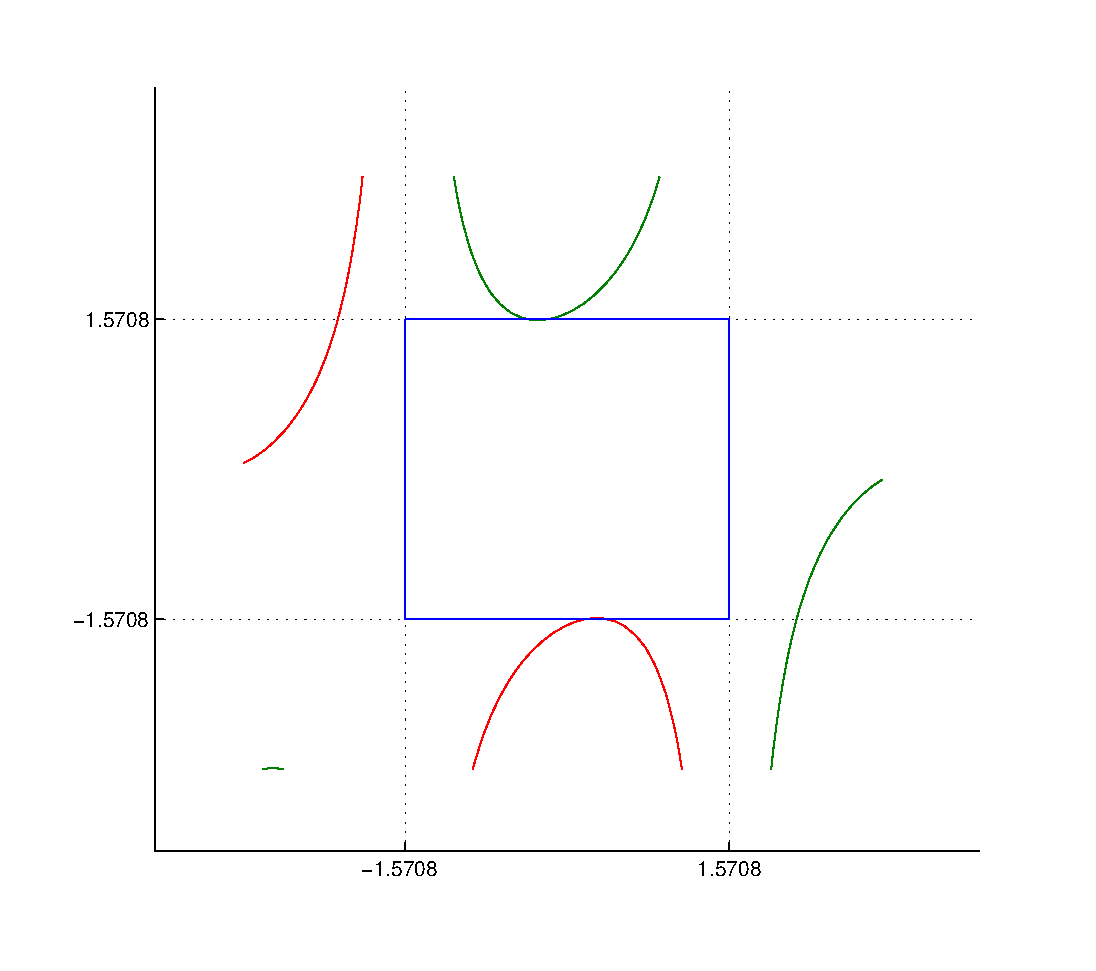
\includegraphics[width=10cm]{phik_hk_ex_LPJ12}
	\caption{Região $\Phi_k$ limitada por $\dot{h}_k$, $\Phi_k$ é apresentado em azul, $\dot{\alpha}_1$ em vermelho e $\dot{\alpha}_2$ em verde}
	\label{fig:hk_phik}
\end{figure}

A Figura \ref{fig:hk_phik} mostra a região $\Phi_k$ limitada pela variação das funções de pertinência do modelo fuzzy T-S para o Exemplo\ref{sec:ex2_JPJ12_again}, considerando-se toda a região de modelagem $C$. Para se obter $\Phi_k$, primeiramente derivaram-se as funções de associação $\alpha_1$ e $\alpha_2$ do sistema, as quais equivalem a, respectivamente,
\begin{equation}\label{eq:func_assoc_LPJ12}
\alpha_1(x) = \alpha_1(z(t)) = \dfrac{1+\sin(x_1(t))}{2}\qquad \alpha_2(x) = \alpha_2(z(t)) = 1 - \alpha_1(z(t))
\end{equation}
A variação de $\alpha_k$ é dada segundo a relação a seguir, considerando a regra da cadeia para derivadas.
\begin{equation}\label{eq:diff_alpha}
\dot{\alpha}_k(x) = \dfrac{d\alpha_k(x)}{dx} \dot{x}.
\end{equation}
Considerando o modelo não linear do sistema, tem-se que $\dot{x} = Ax$, substituindo essa igualdade na Equação \ref{eq:diff_alpha}, temos que
\begin{equation}\label{eq:diff_alpha}
\dot{\alpha}_k(x) = \dfrac{d\alpha_k(x)}{dx} \dot{x}.
\end{equation}
Sabendo que o modelo não linear do Exemplo em questão é dado por
\begin{equation*}
\mathbf{\dot{x} = \begin{bmatrix} -2 & 4\\  -1 - \dfrac{\lambda (1 - sen(x_1))}{2} & -2 \end{bmatrix}x_1}
\end{equation*}
Então, tem-se que
\begin{equation}\label{eq:dot_h_1}
\dot{\alpha}_1 = \dfrac{\cos(x_1)}{2}(-2x_1+4x_2)
\end{equation}
\begin{equation}\label{eq:dot_h_2}
\dot{\alpha}_2 = \dfrac{\cos(x_1)}{2}(-1-\dfrac{\lambda (1-\sin(x_1))}{2})x_1-2x_2)
\end{equation}

Para obter os valores máximos e mínimos das variações de $\alpha_k$, variou-se $x_1$ e $x_2$ dentro da faixa de valores definidos para estes em $C$, com $\alpha_{1_{min}} = \alpha_{2_{min}} = 0$ e $\alpha_{1_{max}} = \alpha_{2_{max}} = 3.2657$. Observe que, se plotada em torno da origem, a região de $\Phi_k$ equivale a $C$.

Para este valor de $\Phi_k$ máximo, para $\lambda = 20$ e para o modelo fuzzy T-S obtido para o setor local $C$, as LMIs do Teorema \ref{th:theorem_6} não geraram solução, de forma que se conclui que a origem do sistema não é estável para esta região. Reduzindo-se a região de definição do sistema gradativamente, tal que se diminui-se o valor de $\Phi_k$ da mesma maneira, obteve-se que o sistema é instável para $\lambda = 20$ somente para a regiões menores ou iguais a $0.51C$.

Para este método em especial, além do parâmetro $\lambda$ que pode ser variado, a análise da estabilidade do sistema depende também de $\Phi_k$, pois este pode ser variado dentre a faixa de valores máximo e mínimo obtido da variação das $h_k$, que por sua vez variam para cada região contida em $C$. Desta maneira, o procedimento adotado para se obter os limites superiores e inferiores de $\lambda$ consistirá em variar a região limitada por $\dot{h}_k$, resolvendo-se as Equações \ref{eq:dot_h_1} e \ref{eq:dot_h_2} para regiões cada vez menores contidas em $C$, de forma a se obter um valor diferente de $\Phi_k$ e assim obter os valores máximos e mínimos de $\lambda$ para cada um dos valores de $\Phi_k$.

Como sabe-se que $\Phi_k$ está contido no intervalo $[0, \pi]$, pois foram os valores obtidos para o melhor caso, em que se considera toda a região $C$, pode-se assumir esta faixa de valores, sem se precisar resolver novamente $\dot{h}_k$, para se obter os valores máximos e mínimos de $\lambda$ para cada valor de $\Phi_k$.

Logo, primeiramente definiu-se $\Phi_k = 0.1$ e variou-se $\lambda$ a partir de $0$, em passos de $0.1$, até o valor máximo para o qual o sistema permanecesse estável. Em seguida aumento-se $\Phi_k$ em passos de 0.1 e obtiveram-se os valores máximos de $\lambda$ para os quais se manteve a condição para estabilidade. Para cada valor de $\Phi_k$ obteve-se um limitante superior de $\lambda$ diferente para a estabilidade. De forma análoga obtiveram-se os limitantes de $\lambda$ para cada valor de $\Phi_k$, com a diferença de que a variação dos valores $\lambda$ a partir de $0$ foi feita em passos de $-0.1$.

Verificou-se o valor mínimo de $\lambda$ para o qual a origem permanece como um ponto de estabilidade do sistema para qualquer valor de $\Phi_k$ é igual a $-1.9$. Já o valor máximo de $\lambda$ tal que se garanta a estabilidade varia conforme $\Phi_k$ varia, de forma que se obteve a curva que relaciona estas duas grandezas, conforme mostra a Figura \ref{fig:phi_k_vs_lambda_max}.

\begin{figure}[htbp]
	\centering
	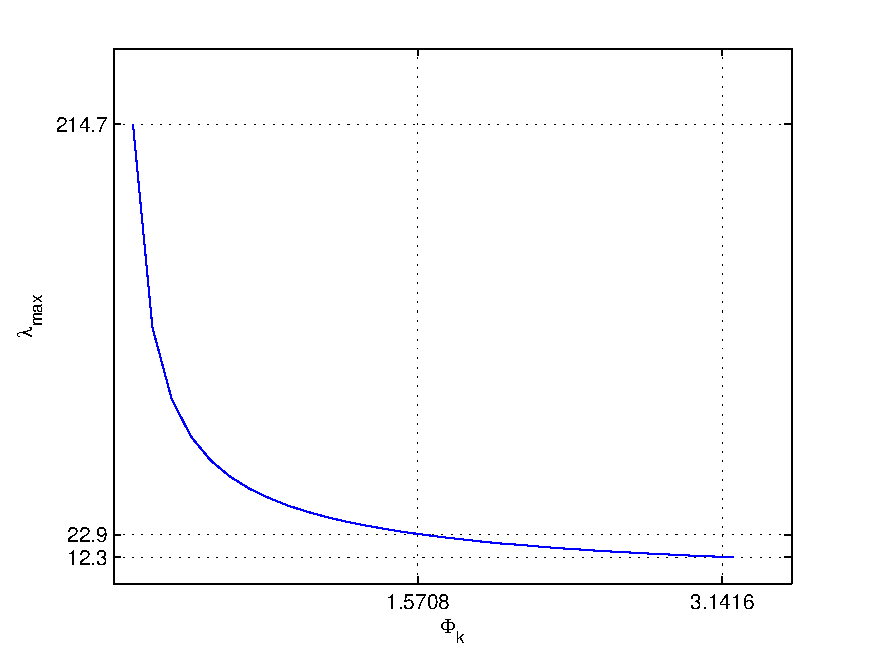
\includegraphics[width=10cm]{phi_vs_lambda_max}
	\caption{$\lambda_{max}$ versus $\Phi_k$}
	\label{fig:phi_k_vs_lambda_max}
\end{figure}

\subsubsection{Método 3: (Método Proposto) Função Lyapunov com $P$ dependente das funções de pertinência e Teorema \ref{th:main_result}}

Ao se utilizar o Teorema \ref{th:main_result}, para verificar se o ponto de equilíbrio na origem é um ponto localmente estável, será necessário obter solução das condições apresentadas neste teorema.

De forma genérica, $P(\alpha)$ é constituído pelo conjunto das matrizes vértices $P_i$, constantes e simétricas, associadas a cada um dos $r$ termos do primeiro simplex $\alpha$, em que $r$ é o número de regras do modelo fuzzy T-S, tais que
\begin{equation}\label{eq:P_alpha}
P(\alpha) = \sum_{i = 1}^{r}\alpha_iP_i
\end{equation}
A matriz $A(\alpha)$ consiste no somatório dos vértices do modelo fuzzy Takagi-Sugeno associados a cada um dos $r$ termos do primeiro simplex, conforme apresentado a seguir.
\begin{equation}\label{eq:A_alpha_eq}
A(\alpha) = \sum_{i = 1}^{r}\alpha_iA_i
\end{equation}
Analogamente, a matriz $X(\alpha)$ é obtida pela combinação de $r$ vértices $X_i$ constantes, mas que não precisam ser simétricos, em função do primeiro simplex $\alpha$.
\begin{equation}\label{eq:X_alpha}
X(\alpha) = \sum_{i = 1}^{r}\alpha_iX_i
\end{equation}
Desta maneira, obtemos para o exemplo em discussão $P(\alpha)$, $X(\alpha)$ e $A(\alpha)$, respectivamente, conforme segue
\begin{equation*}
\begin{array}{lcl}
P(\alpha) & = & \alpha_1P_1 + \alpha_2P_2\\
X(\alpha) & = & \alpha_1X_1 + \alpha_2X_2\\
A(\alpha) & = & \alpha_1\begin{bmatrix}-2&4\\-1&-2\end{bmatrix} + \alpha_2\begin{bmatrix}-2&4\\-(1+\lambda)&-2\end{bmatrix}
\end{array}
\end{equation*}
em que $P_i$ e $X_i, i = 1, 2$  são matrizes $2 \times 2$, correspondentes aos parâmetros a se obter para a análise de estabilidade.

Para obter $J(\theta)$, devemos primeiramente obter as jacobianas de $\alpha = \begin{bmatrix}\alpha_1\\\alpha_2\end{bmatrix}$ em relação a $x = \begin{bmatrix}x_1\\x_2\end{bmatrix}$, as quais correspondem a
\begin{equation*}
\dot{\alpha} = \nabla_x\alpha
\end{equation*}
Assim,
\begin{equation*}
J(x) = \begin{bmatrix}\dot{\alpha}_1\\\dot{\alpha}_2\end{bmatrix}= \begin{bmatrix}\frac{\partial \alpha_1}{\partial x_1}&\frac{\partial \alpha_1}{\partial x_2}\\\frac{\partial \alpha_2}{\partial x_1}&\frac{\partial \alpha_2}{\partial x_2}\end{bmatrix}
= \begin{bmatrix}\dfrac{\cos(x_1)}{2}&0\\\dfrac{-\cos(x_1)}{2}&0\end{bmatrix}
\end{equation*}

Os vértices $J_i$ oriundos de $J(x)$ são obtidos a partir de todas as combinações dos valores limitantes superiores e inferiores de todos os termos dependentes de $x$. É possível identificar que o único termo dependente de $x$ em $J(x)$ é $\cos(x_1)$, que, para a região $C$, tem seus valores máximos e mínimos equivalentes a 1 e 0, respectivamente. Assim, encontramos dois vértices de $J(x)$, os quais são
\begin{equation*}
J_1 = \begin{bmatrix}0&0\\0&0\end{bmatrix}\qquad J_2 = \begin{bmatrix}1&0\\1&0\end{bmatrix}
\end{equation*}
Desta maneira, obtemos $J(\theta)$ como sendo
\begin{equation*}
J(\theta) = \theta_1\begin{bmatrix}0&0\\0&0\end{bmatrix} + \theta_2\begin{bmatrix}1&0\\1&0\end{bmatrix}
\end{equation*}
Como já visto, o sistema possui dois vértices em $P$, os quais são $P_1$ e $P_2$. Além disso, o poliédro em função dos vértices que representa a região $C$ de modelagem do sistema fuzzy T-S é dado por
\begin{equation*}
\chi = co\begin{Bmatrix}x^1,x^2,x^3,x^4\end{Bmatrix} = co\begin{Bmatrix}
\begin{bmatrix}-\pi/2\\-\pi/2\end{bmatrix},\begin{bmatrix}-\pi/2\\\pi/2\end{bmatrix},\begin{bmatrix}\pi/2\\-\pi/2\end{bmatrix},\begin{bmatrix}\pi/2\\\pi/2\end{bmatrix}
\end{Bmatrix}
\end{equation*}
A partir disso, podemos obter $Q(\gamma)$, o qual possui $4$ vértices, conforme a quantidade de vértices de $\chi$, conforme segue.
\begin{equation*}
Q(\gamma) = \gamma_1\begin{bmatrix}P_1x^1&P_2x^1\end{bmatrix}+\gamma_2\begin{bmatrix}P_1x^2&P_2x^2\end{bmatrix}+\gamma_3\begin{bmatrix}P_1x^3&P_2x^3\end{bmatrix}+\gamma_4\begin{bmatrix}P_1x^4&P_2x^4\end{bmatrix}
\end{equation*}

Obtidos todos os termos da LMI \ref{eq:th1_stability}, estaríamos prontos para resolvê-la. Porém, para se obter a solução correta da LMI, considerando os três simplexes $\alpha$, $\theta$ e $\gamma$, é preciso colocar todos os termos da LMI em função de todos os simplexes, isto porque as ferramentas utilizadas para resolver as LMIs neste trabalho não permitem a solução de LMI com termos dependentes de simplexes diferentes entre si.

Na Equação \ref{eq:P_alpha}, por exemplo, temos que $P(\alpha)$ é dependente do primeiro simplex $\alpha$, o grau de relação de $\alpha$ com os vértices de $P(\alpha)$ é de ordem 1. Podemos representar $P(\alpha)$ também em função dos demais simplexes $\theta$ e $\gamma$, sem que haja perda de generalidade, uma vez que $\sum_{i = 1}^{\vartheta}\theta_i = 1$ e $\sum_{i = 1}^{\Gamma}\gamma_i = 1$, da mesma maneira que $\sum_{i = 1}^{r}\gamma_i = 1$. Assim,
\begin{equation}\label{P_multiple_simplexes}
P(\alpha) = \sum_{i = 1}^{r}\alpha_iP_i = P(\alpha, \theta,\gamma) = \sum_{i = 1}^{r}\alpha_i\sum_{i = j}^{\vartheta}\theta_j\sum_{k = 1}^{\Gamma}\gamma_kP_i
\end{equation}

Portanto, para que $ P(\alpha, \theta,\gamma)$ equivalha a $P(\alpha)$, basta assumir o grau de $\theta$ e $\gamma$ como sendo igual a 0 para este termo. Seguindo este mesmo procedimento, encontramos todos os demais elementos da LMI em função de todos os três simplexes do sistema. Agora, finalmente, as LMIs do Teorema \ref{th:main_result} podem ser resolvidas para verificar se o sistema é estável segundo esta abordagem para a região de validade do sistema $C$.

Este método permitiu verificar que o sistema é estável na região $C$ para $\lambda = 20$.

Assim como se fez para os demais métodos, é possível obter os limitantes superiores e inferios de $\lambda$ para os quais o sistema permanece estável para a região $C$ na qual os estados do sistema são válidos e para as quais o modelo fuzzy Takagi-Sugeno fora obtido.

Observou-se que para este método não há um limitante superior de $\lambda$ para o qual a origem se torne instável na região $C$. Por outro lado, valor mínimo de $\lambda$ tal que a origem se mantém estável equivale a $-0.8000$.

\subsubsection{Comparação entre os métodos}

Na Seção \ref{sec:resultado_principal} foi apresentado o resultado principal deste trabalho, que consiste na formulação de um novo método para determinação de estabilidade de sistemas não lineares modelados como sistemas fuzzy Takagi-Sugeno utilizando-se a teoria de estabilidade de Lyapunov via LMIs. A proposta desta seção é comparar o método proposto com outros métodos, a fim de se verificar se essa nova técnica de obtenção de estabilidade é realmente mais relaxada que demais técnicas propostas na literatura. Estes outros métodos da literatura correspondem aos Métodos 1 e 2 apresentados acima. A comparação entre os métodos será feita com base na obtenção dos resultados da aplicação de cada um destes métodos no Exemplo \ref{example_LPJ12}, que é dependente do parâmetro $\lambda$. 

O critério para se determinar qual o melhor método consiste, primeiramente, na verificação de qual método garante a estabilidade assintótica para a maior região do espaço de estados, sendo este o método a ser considerado menos conservador. Em seguida, será feita a comparação  entre os valores máximo e mínimo de $\lambda$ obtidos por cada método para os quais o sistema permanece estável. Este critério de comparação é baseado em na referência bibliográfica \cite{MPSM:2009}.


Nesta seção pôde-se comparar o método de análise de estabilidade de Lyapunov via LMIs aqui proposto com outros métodos já existentes na literatura. Utilizou-se dois métodos para este procedimento, o primeiro método consistiu na análise de estabilidade considerando-se $P$ constante, segundo proposto por (Boyd, 1994 \cite{bookboydl:1994}), o segundo método foi proposto por (Mozelli, Palhares, Sousa e Mendes, 2009 \cite{MPSM:2009}) e nele se considera $P(\alpha)$ e limitante simples das derivadas. Além disso, nomeou-se o método introduzido neste trabalho como Método 3.

Fixando-se $\lambda$ = 20, observou-se que os Métodos 1 e 2 não garantem a estabilidade do sistema para toda a região $C$ para a qual o sistema é definido; ao contrário do Método 3, que garante estabilidade para esta região e este valor de $\lambda$. O Método 1 só garante estabilidade para $\lambda = 20$ para regiões menores ou iguais $0.46C$, enquanto que para o Método 2 o sistema já apresenta valores estáveis para regiões menores ou iguais a $0.51C$.

A busca pelos valores máximo e mínimo de $\lambda$ para os quais o sistema é estável considerando toda a região $C$ permitiu verificar qual dentre os três métodos gera melhores resultados. Para o limitante superior de $\lambda$, verificou-se que o Método 3 garante estabilidade para seja qual for o valor de $\lambda_{max}$, enquanto o Método 1 se limita a $\lambda_{max} = 9.6000$ e o Método 2, para o melhor caso, em que $\Phi_k$ é mínimo, é limitado em $\lambda_{max} = 214.7000$. Assim, o Método 3 gera os melhores resultados para a estabilidade do ponto de equilíbrio na origem, considerando o limitante superior de $\lambda$.

Para o limitante inferior de $\lambda$, obteve-se que os Métodos 1 e 2 são estáveis na região $C$ para valores de $\lambda_{min}$ maiores ou iguais a $-1.9000$. O Método 3, por sua vez, garante a estabilidade apenas para $\lambda \geq -0.8000$. Logo, o Método 3 gera o pior resultado para o limitante inferior de $\lambda$.

\subsection{Exemplo Sistema {\it Droop}}

Uma vez comprovado que o método proposto nos resultados principais provê o melhor resultado para a análise de estabilidade de sistemas dinâmicos, quando comparado com os Métodos 1 e 2, e para $\lambda > 0$, este método será utilizado para a análise de estabilidade de sistemas com dinâmica fuzzy T-S.

Nesta seção serão apresentados os resultados de análise de estabilidade dos Exemplos \ref{ex:droop_UFSM_fuzzyTS} e \ref{ex:4_tanques}, que equivalem, respectivamente ao sistema do inversor de tensão e ao processo de quatro tanques vistos no capítulo anterior.

\begin{example}[Sistema {\it Droop}] \label{ex:estab_sist_droop}
No Exemplo \ref{ex:droop_UFSM_fuzzyTS} foi apresentada a modelagem fuzzy T-S do sistema do inversor de tensão, agora será feita a análise de estabilidade deste sistema, utilizando o modelo proposto no Teorema \ref{th:main_result}. Será verificado se o sistema é estável para a região definida por $C = \{x(t) \in \rm I\!R^3 | x_1(t) = P_f \in [0; 25000], x_2(t) = Q_f \in [-70000; 5000], x_3(t) = \delta \in [-0.02; 0.1]\}$.
\end{example}

Para tanto, é preciso encontrar uma solução para as LMIs propostas no Teorema \ref{th:main_result}, de forma que obtenha $P > 0$. Os parâmetros da LMI\ref{eq:th1_stability} para este exemplo são obtidos conforme segue.

Sabendo-se que o modelo fuzzy T-S do sistema possui 16 vértices $A_i$ e 16 fun\~{c}ões de associação $\alpha_i, i = 1, \hdots, 16$, com $A_i$ e $\alpha_i$ obtidos no capítulo anterior,$A(\alpha)$ é dado por
\begin{equation*}
A(\alpha) = \sum_{i = 1}^{16}\alpha_iA_i
\end{equation*}
De forma análoga, $P(\alpha)$ é obtido como
\begin{equation*}
P(\alpha) = \sum_{i = 1}^{16}\alpha_iP_i
\end{equation*}
Em que $P_i, i = 1,\hdots, 16$ são matrizes simétricas a serem determinadas. $X_i, i = 1,\hdots,16$ também são matrizes, porém náo simétricas a serem determinadas, tais que
\begin{equation*}
X(\alpha) = \sum_{i = 1}^{16}\alpha_iX_i
\end{equation*}
Para obter o termo $J(\theta)$, primeiramente é preciso obter as jacobianas de $\alpha$. Por possuir 16 regras fuzzy, o que resulta em 16 funções de pertinência, e por possuir três vairáveis de estado, a jacobiana $J$ será uma matriz de dimensão $16 \times 3$. O termo $J(\theta)$ terá $2^m$ \v{e}rtices, em que $m$ é o número de não linearidades da jacobiana J.

A função de pertinência $\alpha_1$, por exemplo, equivale a
\begin{equation*}
\alpha_1(z) = M_{11}M_{12}M_{13}M_{14}
\end{equation*}
Neste exemplo, os graus de pertinência são dependentes unicamente do estado $x_3$. Assim, a jacobiana de $\alpha_1$ será dada por
\begin{equation*}
\alpha_1(z) = \begin{bmatrix}0&0&\frac{\partial\alpha_1(z)}{\partial x_3}\end{bmatrix}
\end{equation*}
Em que 
\begin{equation*}
\frac{\partial\alpha_1(z)}{\partial x_3} = \dot{M}_{11}M_{12}M_{13}M_{14}+M_{11}\dot{M}_{12}M_{13}M_{14}+M_{11}M_{12}\dot{M}_{13}M_{14}+M_{11}M_{12}M_{13}\dot{M}_{14}
\end{equation*}
Os graus de pertinência $M_{ij}$ são dados por
\begin{equation*}
M_{1i} = \dfrac{z_i-min(z_i)}{\Delta z_i}\qquad M_{2i}= 1 -  M_{1i}
\end{equation*}
Assim,
\begin{equation*}
\dot{M}_{1i} = \dfrac{\dot{z_i}}{\Delta z_i} = -\dot{M}_{2i}
\end{equation*}
Sabendo-se que
\begin{equation*}
z_1 = \cos(x_3) \Rightarrow \dot{z}_1 = -\sin(x_3)\qquad z_3 = \sin(x_3) \Rightarrow \dot{z}_3 = \cos(x_3)
\end{equation*}
Logo tem-se que
\begin{equation*}
\dot{z}_1 = -z_3\quad\text{e}\quad\dot{z}_3 = z_1
\end{equation*}
Das relações acima, tem-se que
\begin{equation*}
\dot{M}_{11}= -\dfrac{\dot{z_3}}{\Delta z_1}
\end{equation*}
Como
\begin{equation*}
{M}_{13}= -\dfrac{z_3-min(z_3)}{\Delta z_3}\Rightarrow z_3 = {M}_{13}\Delta z_3+min(z_3)
\end{equation*}
Logo,
\begin{equation*}
\dot{M}_{11} = -{M}_{13}\dfrac{\Delta z_3}{\Delta z_1}-\dfrac{min(z_3)}{\Delta z_1}
\end{equation*}
De forma análoga,
\begin{equation*}
\dot{M}_{13} = {M}_{11}\dfrac{\Delta z_1}{\Delta z_3}-\dfrac{min(z_1)}{\Delta z_3}
\end{equation*}
Assim, $\dot{\alpha}_i(z)$ pode ser reescrito como

\begin{align*}
\frac{\partial\alpha_1(z)}{\partial x_3} &= (-{M}_{13}\dfrac{\Delta z_3}{\Delta z_1}-\dfrac{min(z_3)}{\Delta z_1})M_{12}M_{13}M_{14}+M_{11}\dot{M}_{12}M_{13}M_{14}\\
&+ M_{11}M_{12}({M}_{11}\dfrac{\Delta z_1}{\Delta z_3}-\dfrac{min(z_1)}{\Delta z_3})M_{14}+M_{11}M_{12}M_{13}\dot{M}_{14}
\end{align*}
Assim, é possível verificar que $\frac{\partial\alpha_1(z)}{\partial x_3}$ é dependente de 6 termos não lineares, os quais são
\begin{equation*}
M_{11}, M_{12}, M_{13}, M_{14}, \dot{M}_{12}, \dot{M}_{14}
\end{equation*}

As demais derivadas parciais de $\alpha$ são obtidas com base nos mesmos princípios, obtendo-se os mesmos termos não lineares de $\alpha_1$.

Finalmente, como os vértices de $J(\theta)$ são dependentes de 6 termos não lineares distintos, foram obtidos os 64 vértices de $J(\theta)$, oriundos de todas as combinações possíveis dos valores máximos e mínimos das não linearidades de J.

Para a obtenção do termo $Q(\gamma)$ é preciso primeiramente obter a representação por vértices do poliédro $\chi$ contido na região limitada pelos valores máximos e mínimos das variáveis de estado. Assim, obtém-se
\begin{align*}
\chi &= co\begin{Bmatrix}x^1,x^2,x^3,x^4,x^5,x^6,x^7,x^8\end{Bmatrix}\\
 &= co\begin{Bmatrix}
\begin{bmatrix}0\\-70000\\-0.02\end{bmatrix}, \begin{bmatrix}0\\-70000\\ 0.1\end{bmatrix}, \begin{bmatrix}0\\5000\\ 0.1\end{bmatrix}, \begin{bmatrix}0\\5000\\ -0.02\end{bmatrix}, \begin{bmatrix}25000\\-70000\\-0.02\end{bmatrix}, \begin{bmatrix}25000\\-70000\\ 0.1\end{bmatrix}, \begin{bmatrix}25000\\5000\\ 0.1\end{bmatrix}, \begin{bmatrix}25000\\5000\\ -0.02\end{bmatrix}
\end{Bmatrix}
\end{align*}
O parâmetro $Q(\gamma)$, portanto, terá 8 vértices, dados por

\begin{equation*}
Q(\gamma) = \gamma_1\begin{bmatrix}P_1x^1&P_2x^1&\hdots&P_16x^1\end{bmatrix}+\gamma_2\begin{bmatrix}P_1x^2&P_2x^2&\hdots&P_16x^2\end{bmatrix}+\hdots+\gamma_8\begin{bmatrix}P_1x^8&P_2x^8&\hdots&P_{16}x^8\end{bmatrix}
\end{equation*}


Obtidos todos os termos das LMIs de análise de estabilidade do Teorema \ref{th:main_result}, é necessário colocá-los em função dos três simplexes $\alpha$, $\theta$ e $\gamma$, o que foi feito conforme mostrou a Equação \ref{P_multiple_simplexes}.

Resolvendo-se as LMIs do Teorema \ref{th:main_result}, verificou-se que o sistema é estável para a região $C$ para a qual foi definido.

\section{Considerações Finais}

Neste capítulo foi proposto um novo método para determinação de estabilidade de Lyapunov via LMIs de sistemas dinâmicos não lineares como sistemas fuzzy Takagi-Sugeno pelo método de não linearidade de setor. Foi proposto o Teorema \ref{th:main_result}, para o qual esperou-se obter resultados menos conservadores para a análise de estabilidade do sistema. O Exemplo \ref{example_LPJ12} foi utilizado para a aplicação do Teorema proposto. Verificou-se, por meio deste teorema, que a origem é um ponto de equilíbrio estável, considerando-se $\lambda = 20$, para toda a região $C$ para a qual os estados do sistema são definidos.

Para se este método é, de fato, menos conservador que outros métodos existentes na literatura, foi realizada a análise de estabilidade deste mesmo sistema por meio de outros dois métodos. O primeiro dentre estes Métodos consistiu utilização do método de Lyapunov para $P$ constante e dinâmica fuzzy T-S. Para este método, verificou-se que a origem somente é um ponto estável do sistema, com $\lambda = 20$, para regiões menores ou iguais a $0.46C$, em que $C$ é a região de validade do sistema no plano de estados.

O segundo método consistiu na análise de estabilidade para o sistema com $P$ dependente das funções de associação $\alpha$ do modelo fuzzy T-S, porém considerando-se a configuração por limitantes simples das derivadas, conforme proposto na referência \cite{MPSM:2009}. Pra este método, verificou-se o que, para $\lambda = 20$, a origem somente é um ponto de equilíbrio estável para regiões menores ou iguais a $0.51C$.

Utilizando-se o critério da região para a qual o ponto de equilíbrio é estável para cada método, como o Teorema proposto neste capítulo garantiu a estabilidade para uma região maior que os demais, verificou-se que este método é de fato mais relaxado.

Outro parâmetro de comparação utilizado foi, fixando-se a região $C$ de validação, qual seriam os valores de $\lambda$ máximo e mínimo para os quais o sistema seja estável nesta região do plano de estados. Verificou-se que para o limitante inferior, o Teorema \ref{th:main_result} produziu o pior resultado, já que deixou de ser estável para um valor maior de $\lambda$ quando comparado com os demais métodos, uma vez que obteve $min(\lambda) = -0.8000$, enquanto os demais métodos apresentaram $min(\lambda) = -1.9000$. Por outro lado, o Teorema \ref{th:main_result} se mostrou ser o melhor método para a determinação da estabilidade, uma vez que não fora encontrado limitante superior de $\lambda$ a partir de qual a origem deixasse de ser um ponto de equilíbrio assintoticamente estável.

% *** Região de atração ***
\chapter{Estimativa de Região de Atração}\label{cap_RegAtrac}

\section{Introdução}

Ao se analisar a estabilidade de sistemas dinâmicos, muitas vezes não é suficiente apenas saber se um determinado ponto de equilíbrio é estável dado o domínio definido para o respectivo sistema. É preciso também saber a região dentro da qual o ponto de equilíbrio é estável, ou seja, a região dentro da qual qualquer trajetória que a adentrar jamais conseguirá sair dela, mantendo-se a partir daí sempre próximo ao ponto de equilíbrio contido naquela região. Esta região que contém o ponto de equilíbrio e todas as trajetórias que jamais se afastam deste, e, no caso de estabilidade assintótica, sempre tendem a este, é dita região, ou domínio, de atração.

O objetivo deste capítulo é obter a estimativa a região de atração de sistemas dinâmicos. No capítulo anterior foi proposto um novo método para análise de estabilidade utilizando o teorema de Lyapunov e fazendo-se uso de Desigualdades Matriciais Lineares. No decorrer deste capítulo pretende-se obter a estimativa da região de atração para o resultado obtido pelo método de análise de estabilidade proposto no capítulo anterior, assim como para os demais métodos utilizados para comparação com o resultado principal do último capítulo. Deste modo, será introduzido um novo critério de comparação entre os métodos de análise de estabilidade propostos. Também será verificada a estimativa da região de atração do sistema linearizado em torno da origem, técnica que também será utilizada para comparação com o método proposto neste trabalho para análise de estabilidade.

\section{Estimativa de Região de Atração}

Retomando o exemplo do pêndulo invertido sem atrito visto no capítulo anterior, no qual foi mostrado que o ponto de equilíbrio na origem é estável para este sistema. Observando o retrato de fase obtido do modelo, é possível verificar que as trajetórias das respostas nem sempre convergem para a origem, mostrando que este ponto de equilíbrio não é estável para todo o domínio definido no plano de estados para este sistema. A Figura \ref{fig:reg_atrac_pend} mostra o  retrato de fase do pêndulo invertido sem atrito e ilustra a estimativa do domínio de atração da origem.
\begin{figure}[htbp]
	\centering
	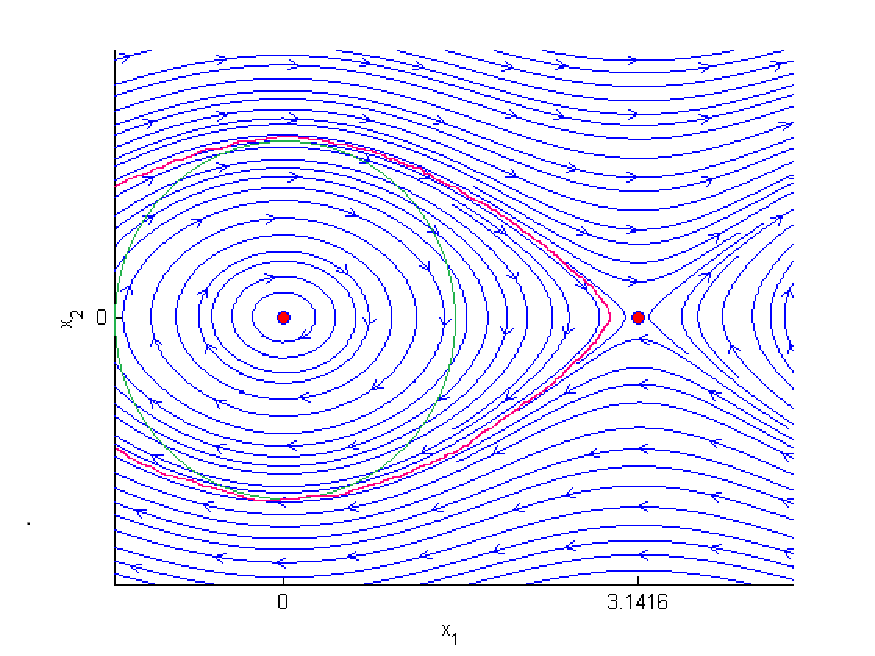
\includegraphics[width=10cm]{reg_atrac_pend}
	\caption{Estimativa da região de atração para o exemplo do pêndulo simples sem atrito}
	\label{fig:reg_atrac_pend}
\end{figure}
O domínio de atração completo deste ponto do equilíbrio situado na origem está representado pela região contida pela curva de cor rosa. A curva verde, porém, representa a estimativa do domínio de atração a qual será objeto de estudo deste capítulo.

Observe que, como o atrito é desconsiderado, a energia total do sistema permanece constante, como já visto anteriormente, a qual pode ser representada por $E(x) = c$, e forma um contorno fechado em torno da origem do plano de estados. Quando se considera o atrito, $E(x)$ se comporta como uma espiral, que se aproxima cada vez mais da origem. Para cada instante de tempo $E(x)$ vai diminuindo mais, até que alcança a origem do plano de estados. A estimativa do domínio de atração, neste caso, consiste em obter o raio $c$ máximo para o qual o sistema permanece estável para qualquer instante de tempo. De forma semelhante, Lyapunov provou que a função quadrática $V(x)$ contínua no tempo, existe uma região no plano de estados tal que $V(x) < c$ quando $\dot{V}(x) < 0$. A superfície expressa por $V(x) = c$ é conhecida como superfície de Lyapunov, para algum $c > 0$ \cite{bookkhalil:2003}.

A superfície de Lyapunov sempre estará em torno da origem do plano de estados e pode apresentar forma elipsoidal ou circular. Com base nesta afirmação, pode-se concluir que o conjunto de todos os vetores $x$ tais que $V(x) = c$, $c$ constante positivo qualquer, formam uma elipse quando a matriz simétrica $P$ da função de Lyapunov for definida positiva ($P > 0$) \cite{bookboydl:1994}. Os semi-eixos da elipse são $1/\sqrt(\lambda_i)$, em que $\lambda_i$ são os autovalores de $P/c$.

Portanto, o domínio de atração é dado pelo maior subnível da função de Lyapunov contido na região de estados limitada pelos limitantes das variáveis de estados para a qual o sistema é estável. Logo, se existem matrizes $P(\alpha) = P(\alpha)' > 0$ e $V(x) = x'P(\alpha)x$ tal que $\dot{V}(x) < 0$, então o maior conjunto contido no politopo $\chi$, em que $\chi$ é o politopo para o qual $\dot{V}(x) < 0$, é definido por
\begin{equation} \label{eq:Omega}
\Omega = \{x \in \rm I\!R^{n} | x'P(\alpha)x \leq 1\}
\end{equation}

As subseções a seguir apresentam duas abordagens para a obtenção da melhor estimativa da região de atração de sistemas com a origem como um ponto localmente assintoticamente estável.

\subsection{Primeira abordagem para obtenção da estimativa da região de atração}

Uma outra representação para o poliedro $\chi$, que equivale ao politopo dentro do qual se obteve o modelo do sistema, é dada por
\begin{equation}\label{eq:anothe_rep_of_chi}
\chi = \{x \in \rm I\!R^{n} | Qx \preceq \textbf{q}\}
\end{equation}
em que $Q\in\rm I\!R^{g\times n}$, $n\leq g$, $rank(Q) = n$, $\textbf{q} \in \rm I\!R^{n}$, $q_{(i)} > 0$, tal que $q_{(i)}$ é cada elemento de $\textbf{q}$, com $0 \in \chi$.
\begin{observation}
	Para qualquer vetor $x \in \rm I\!R^{g}$, $x \succeq 0$ significa que todos os componentes de $x$, denotados $x_{(i)}$ são não negativos. Para $x$, $y \in \rm I\!R^{n}$, $x \succeq y$ implica que $x_{(i)} - y_{(i)} \geq 0$, para todo $i = 1,\hdots, n$. Além disso, $A_{(i)}$ refere-se à i-ésima linha da matriz $A$.
	
	Observe que pode-se também ter
	\begin{equation}\label{eq:another_rep_of_chi}
	\chi = \{x \in \rm I\!R^{n} |-\mu\preceq x \preceq\mu\}
	\end{equation}
	onde $\mu \in \rm I\!R^{n}$ e $\mu{(i)} > 0, i = 1, \hdots,n$.
	De fato, os vértices $x^k$ são obtidos de $\mu$ pela combinação linear\cite{article:tarbouriech:2009}
	\begin{equation*}
	x^k = D_j\mu,\quad j =1,\hdots,2^n
	\end{equation*}
	onde $D_j, j = 1,\hdots,2^n$ são matrizes diagonais no domínio $\rm I\!R^{n \times n}$, constituídas por todas as combinações  formadas com $1$ e $-1$.
\end{observation}
Assim, uma estimativa da região de atração para o sistema não linear \ref{eq:nonlinear_system_cap_stability} pode ser obtida por um problema de minimização, conforme enuncia o teorema proposto a seguir.
	\begin{theorem}[Estimativa para região de atração] \label{th:reg_atrac_1}
		Se existem matrizes $P(\alpha) = P(\alpha)' > 0$, $X(\alpha)$, 
		$T$, um  escalar $\gamma >0$ e dado os parâmetros de ponderação $\omega_1$ e $\omega_2$ tais que
		\begin{equation}\label{eq:another_condition_1}
		min\{\omega_1Trace(T) +\omega_2\gamma\}
		\end{equation}
		sujeito a
		\begin{equation}\label{eq:th1_stability2}
		A(\alpha)'P(\alpha) + P(\alpha)A(\alpha) + Q(\gamma)J(\theta)A(\alpha) + X(\alpha)\textbf{1}'J(\theta)A(\alpha) + A(\alpha)'J(\theta)'\textbf{1}X(\alpha)' < 0
		\end{equation}
		\begin{equation}\label{eq:another_condition_3}
		\begin{bmatrix}P(\alpha)\mu_{(i)}&I^{(i)'}\\\textbf{*}&\gamma\mu{(i)}\end{bmatrix} \geq 0,\quad i = 1, ..., n
		\end{equation} 
		\begin{equation}\label{eq:another_condition_2}
		\begin{bmatrix}T&P(\alpha)\\P(\alpha)&P(\alpha)\end{bmatrix} \geq 0,
		\end{equation}	
		para todo $\alpha \in \Lambda_r$, $\theta \in \Lambda_{\vartheta}$ e $\gamma \in\Lambda_{\nu}$, 
		então 
		a origem é um ponto de equilíbrio assintoticamente localmente estável
		para o sistema não linear \ref{eq:nonlinear_system_cap_stability}
		no conjunto invariante do domínio de atração
		$\Omega = \{x\in\rm I\!R^{n}| x'P(\alpha)x \leq \gamma^{-1}\}\subseteq \chi$.
	\end{theorem}
	\begin{proof}
		Seja a função de Lyapunov $V(x)=x'P(\alpha)x$ com $P(\alpha)>0$.
		Conforme o Teorema~\ref{th:main_result}, a condição
		\ref{eq:th1_stability2} assegura $\dot{V}(x)<0$ e 
		portanto o modelo fuzzy Takagi-Sugeno \ref{eq:fuzzy_TS_system_cap_stability} é assintoticamente
		estável.
		%
		Para um politopo $\chi$ dado em \ref{eq:another_rep_of_chi},
		a condição \ref{eq:another_condition_3} assegura que
		$\Omega$ definido em \ref{eq:Omega} está incluso no politopo $\chi$,
		ou seja, $\Omega \subseteq \chi$ \cite{bookboydl:1994}.
		%
		Note que o modelo fuzzy Takagi-Sugeno \ref{eq:fuzzy_TS_system_cap_stability} somente representa 
		\ref{eq:nonlinear_system_cap_stability} para $x\in \chi$.
		Como $\Omega \subseteq \chi$, a função $V(x)$
		é localmente decrescente em $\Omega$ e $x=x(\gamma)$. Assim,
		$\Omega$ é um conjunto invariante em relação
		as trajetórias de \ref{eq:nonlinear_system_cap_stability}
		e portanto é um domínio de estabilidade do sistema não linear.
		As condições \ref{eq:another_condition_1} e \ref{eq:another_condition_2} asseguram a minimização do traço de $P(\alpha)$, 
		pois via complemento de Schur tem-se $T\geq P(\alpha)$, e portanto
		a maximização do volume de $\Omega$ \cite{bookboydl:1994}.
	\end{proof}

Veja que este teorema só é válido para sistemas com estados definidos em uma região simétrica $C$.

\subsection{Segunda abordagem para obtenção da estimativa da região de atração}

A restrição de $\Omega\subset\chi$ é válida se \cite{bookboydl:1994}
\begin{equation}\label{eq:largest_set_eq}
b_k'P(\alpha)^{-1}b_k \leq 1,\quad k = 1, \hdots, q.
\end{equation}

Observe que a Equação \ref{eq:largest_set_eq} não aparece no formato de LMI, para contornar este problema, será utilizado o Complemento de Schur, enunciado no Lema a seguir.

\begin{lemma}[Complemento de Schur para desigualdades não restritas] (Boyd, 1994) \cite{bookboydl:1994} Suponha $Q$ e $R$ matrizes simétricas. A condição
	\begin{equation}\label{eq:schur_compl_nonrestrict_1}
	\begin{bmatrix}
	Q&S\\S'&R
	\end{bmatrix} \geq 0
	\end{equation}
	é equivalente a
	\begin{equation}\label{eq:schur_compl_nonrestrict_2}
	R \geq 0,\quad Q-SR^{-1}S' \geq 0,\quad S(I-RR^{-1}) = 0.
	\end{equation}
	\label{lem:finsler_short_version_nonrestrict_inequalities}
\end{lemma}

Assim, aplicando o Complemento de Schur para desigualdades não restritas, a inequação \ref{eq:largest_set_eq} passa a equivaler à LMI

\begin{equation}\label{eq:largest_set}
\begin{bmatrix}\textbf{1}&b_k'\\b_k&P(\alpha)\end{bmatrix} \geq 0,\quad k = 1, ..., q
\end{equation}

Além disso, a região contida pelo conjunto $\Omega$ pode ser obtida maximizando o raio de $\beta > 0$ da bola centrada na origem do plano de estados contida em $\Omega$, ou seja, obtendo-se $\beta_{min}$ tal que a LMI apresentada na Equação \ref{eq:enlargment_of_largest_set} seja satisfeita.
\begin{equation}\label{eq:enlargment_of_largest_set}
P(\alpha) -  \beta I < 0
\end{equation}
Observe que as LMIs $P>0$ e $\dot{V}(x) < 0$ são suficientes para garantir a estabilidade assintótica do ponto de equilíbrio na origem. A adição das LMIs \ref{eq:largest_set} e \ref{eq:enlargment_of_largest_set} apenas garantem a obtenção de $P$ ótimo para a se obter a maior região de estimativa do domínio de atração, já se assumindo que o sistema é estável. Tem-se então o seguinte teorema proposto.
	\begin{theorem}[Outra estimativa para a região de atração]\label{th:reg_atrac_2} 
		Se existem matrizes $P(\alpha) = P(\alpha)' > 0$, $X(\alpha)$, um  escalar $\beta >0$ tais que
		\begin{equation}\label{eq:condition_1}
		min \quad \beta
		\end{equation}
		sujeito a
		\begin{equation}\label{eq:largest_set2}
		\begin{bmatrix}\textbf{1}&b_k'\\b_k&P(\alpha)\end{bmatrix} \geq 0,\quad k = 1, ..., q
		\end{equation}
		\begin{equation}\label{eq:enlargment_of_largest_set2}
		P(\alpha) -  \beta I < 0
		\end{equation} 
		e a LMI \eqref{eq:th1_stability2} sejam satisfeitas
		para todo $\alpha \in \Lambda_r$, $\theta \in \Lambda_{\vartheta}$ e $\gamma \in\Lambda_{\nu}$, 
		então $\Omega = \{x\in\rm I\!R^{n}| x'P(\alpha)x \leq 1\}\subseteq \chi$ é um conjunto invariante do domínio de atração para o sistema não linear \ref{eq:nonlinear_system_cap_stability} e a origem é um ponto de equilíbrio assintoticamente localmente estável.
	\end{theorem}
	\begin{proof}
		A prova segue linhas semelhantes da prova do Teorema~\ref{th:reg_atrac_1}. 
		A condição \ref{eq:largest_set2} implica $\Omega \subset \chi$ \cite{bookboydl:1994}. A condição \ref{eq:enlargment_of_largest_set2}
		implica $ x'P(\alpha)x < \beta ||x||$ e portanto a curva de nível
		$x'P(\alpha)x=1$ contém a esfera $||x||=1/\beta$ que é maximizada
		por \ref{eq:condition_1}. Dessa forma, o volume de $\Omega$ é maximizado.
	\end{proof}

\section{Exemplos numéricos}

Nesta seção serão utilizados exemplos numéricos já apresentados em capítulos anteriores, para os quais se obterá uma estimativa da região de atração.

%\subsection{Exemplo sistema de segunda ordem}\label{sec:ex2_JPJ12_cap_reg_atrac}

O Exemplo \ref{example_LPJ12} será utilizado nesta seção para se obter a estimativa do domínio de atração para o sistema linearizado em torno da origem, além da estimativa da região de atração para o três métodos de análise de estabilidade do modelo fuzzy T-S equivalente ao modelo não linear vistos no capítulo anterior. Para a estimativa do domínio de atração será aplicado, além das LMIs necessárias e suficientes para determinação da estabilidade em cada Método, o Teorema \ref{th:reg_atrac_1} ou o Teorema \ref{th:reg_atrac_2}. Estes diferentes métodos serão aplicados neste exemplo e, em seguida, seus resultados serão comparados para se reforçar a inspeção de qual dentre estes métodos seria o menos conservador. O critério para comparação utilizado será baseado na estimativa do domínio de atração para cada um dos métodos. Aquele que resultar na melhor estimativa, correspondendo à maior região para o domínio de atração, será considerado o melhor método.

\subsection{Método 1: Estabilidade do sistema com dinâmica linearizada}

Além dos métodos introduzidos no capítulo anterior, será utilizado um novo método neste capítulo, o qual consiste em obter, a partir do modelo não linear, um modelo linearizado segundo as técnicas clássicas encontradas na literatura. Nesta seção será utilizado o método de linearização por série de Taylor.

\subsubsection*{Análise de Estabilidade}

Para a análise da estabilidade do sistema linearizado será aplicada a função de Lyapunov para obtenção de uma matriz $P$ definida positiva, tal que o sistema seja estável.

Conforme estabelecido pela definição da estabilidade de Lyapunov, as LMIs necessárias para a determinação da estabilidade do sistema tal que a matriz $P$ não dependa das funções de pertinência, ou seja, para $P$ constante, equivalem a \cite{bookboydl:1994}

\begin{equation}\label{eq:LMIs_est_met_1}
\begin{cases}
P \geq 0\\
A'P + PA \leq 0
\end{cases}
\end{equation}

em que $A$ é uma matriz pertencente ao $\rm I\!R^{n \times n}$ cujos elementos independem dos estados $n$ do sistema. O  Exemplo \ref{ex:example2_LPJ12_non_linear_system}, quando na forma matricial, como visto anteriormente, possui um elemento não linear dependente do estado $x_1$. Portanto, será necessário linearizar o sistema tal que se obtenha a matriz $A$ no formato requerido por este método.

Para se obter o  modelo linearizado o Exemplo \ref{ex:example2_LPJ12_non_linear_system}, utilizou-se o método de linearização por série de Taylor em torno da origem, também conhecida como série de Maclaurin\footnote{Para se obter o modelo linearizado do sistema, obteve-se a representação deste na forma matricial $\dot{\textbf{x}} = A\textbf{x}$ e aplicou-se a função $taylor(A, x^*)$ do MatLab, em que $x^* = 0$.}.

O modelo linearizado é apresentado na Equação \ref{eq:ex_LPJ12_lin}.
\begin{equation}\label{eq:ex_LPJ12_lin}
\begin{cases}\dot{x}_1 = -2x_1 + 4x_2\\
\dot{x}_2= -(1 + \dfrac{\lambda}{2})x_1 - 2x_2
\end{cases},\qquad \lambda = 20
\end{equation}

Assim, a matriz $A$ do modelo linearizado será dada por

\begin{equation}\label{eq:ex_LPJ12_lin_A}A = \begin{bmatrix}-2&4\\-(1 + \dfrac{\lambda}{2})&-2\end{bmatrix},\qquad \lambda = 20
\end{equation}

Resolvendo as LMIs necessárias para a verificação da estabilidade do modelo linearizado, apresentadas na Equação \ref{eq:LMIs_est_met_1}, verifica-se que o sistema é estável para a região poliédrica $\chi$ e $\lambda = 20$.

\subsubsection*{Estimativa de Região de Atração}

Embora na análise de estabilidade do Método 1 tenha-se visto que o sistema é estável para toda a região $C$ para a qual os estados foram definidos, veremos que esta afirmação não é válida para todo o ponto do plano de estados, uma vez que o modelo linearizado só corresponde ao sistema não linear em pontos próximos à origem. Para tanto, será feita uma varredura do neste plano dentro da região de validade $C$ do sistema, considerando-se a modelagem não linear, e se  investigará em quais pontos a LMI $A'P + PA \leq 0$ é válida para a matriz $P$ obtida da análise de estabilidade do sistema, considerando-se $A$ a matriz do modelo não linear.

O teorema de estabilidade de Lyapunov estabelece, como visto no Teorema \ref{th:lyap_stability} no capítulo anterior que para se garantir a estabilidade assintótica local do ponto de equilíbrio situado na origem, seja $V(x)$ a função de Lyapunov definida positiva e para uma matriz $P > 0$, a variação de $V(x)$ deve ser definida negativa, ou seja, $\dot{V}(x) < 0$. Dito isto, para encontrar a região no plano de estados para a qual o Método 4, de fato, produz um resultado estável, deve-se obter primeiramente a inequação $\dot{V}(x)$.

Sabe-se que o exemplo em estudo possui o modelo não linear $\dot{x} = Ax$ como apresentado a seguir.

\begin{equation}\label{eq:ex2_LPJ12_non_linear_again_again}
\begin{cases}\dot{x}_1 = -2x_1 + 4x_2
\\-(1 + \dfrac{\lambda(1 - \sin(x_1))}{2})x_1 - 2x_2\end{cases},\qquad \lambda = 20
\end{equation}
Vimos anteriormente que, para $P$ constante, tem-se
\begin{equation*}
\dot{V} = x'A'Px +x'PAx < 0
\end{equation*}
O que equivale a
\begin{equation}\label{eq:V_dot_2xPAx}
\dot{V} = -2xPAx < 0
\end{equation}
Foi utilizada a equação \ref{eq:V_dot_2xPAx} substituído $A$ pelo correspondente do modelo não linear do sistema para se obter a região para a qual $\dot{V}(x)$ é definida negativa definida como $D = \{x | \dot{V}(x) < 0\}$. Desta forma, se obteve a região identificada na Figura \ref{fig:reg_estab_Met4}.

\begin{figure}[htbp]
	\centering
	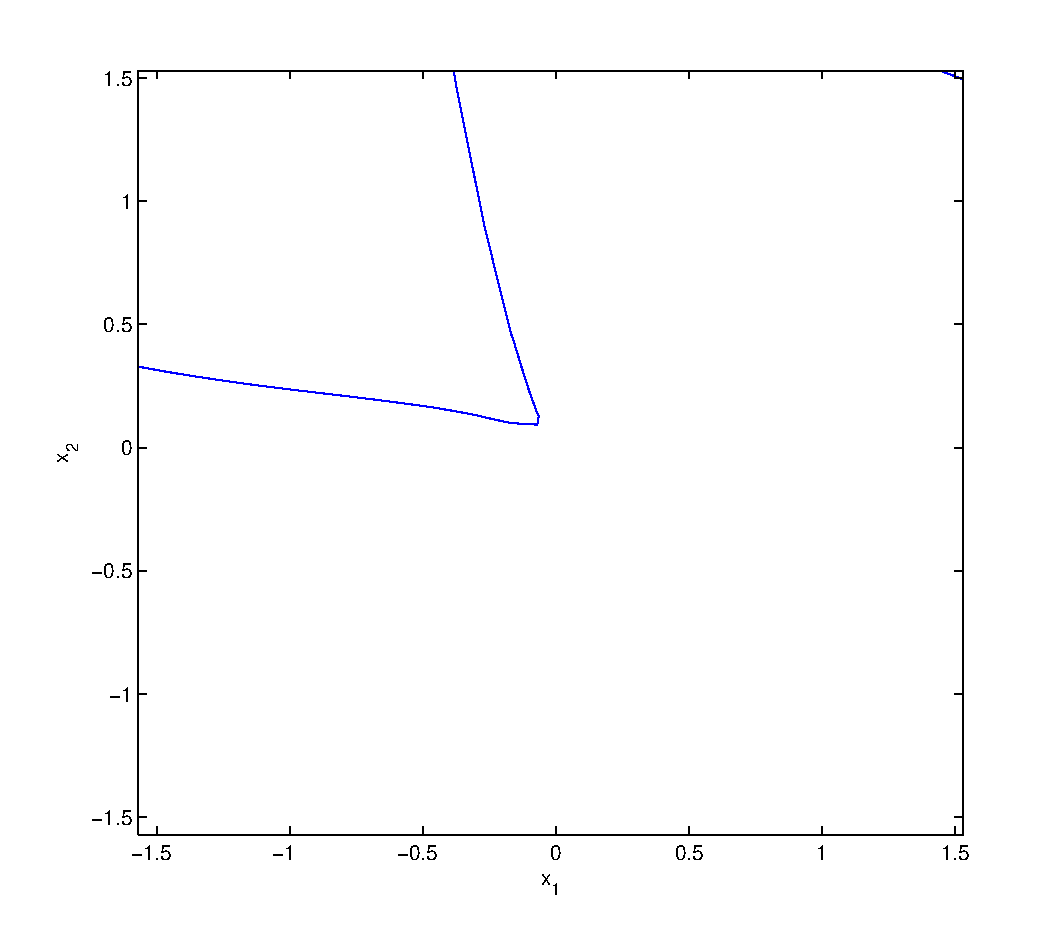
\includegraphics[width=10cm]{reg_estab_Met4}
	\caption{Região $D$ para a qual é válida a relação $\dot{V}(x) < 0$. A região está contida abaixo da curva em azul}
	\label{fig:reg_estab_Met4}
\end{figure}

Para visualizar que a região abaixo da curva azul na Figura \ref{fig:reg_estab_Met4} realmente equivale à região em que $\dot{V}(x) < 0$ para o modelo não linear, foram plotadas várias curvas para $\dot{V}(x) < y$, em que $y$ é o limitante da região representada por cada curva, Figura \ref{fig:V_dot_levels}.

\begin{figure}[htbp]
	\centering
	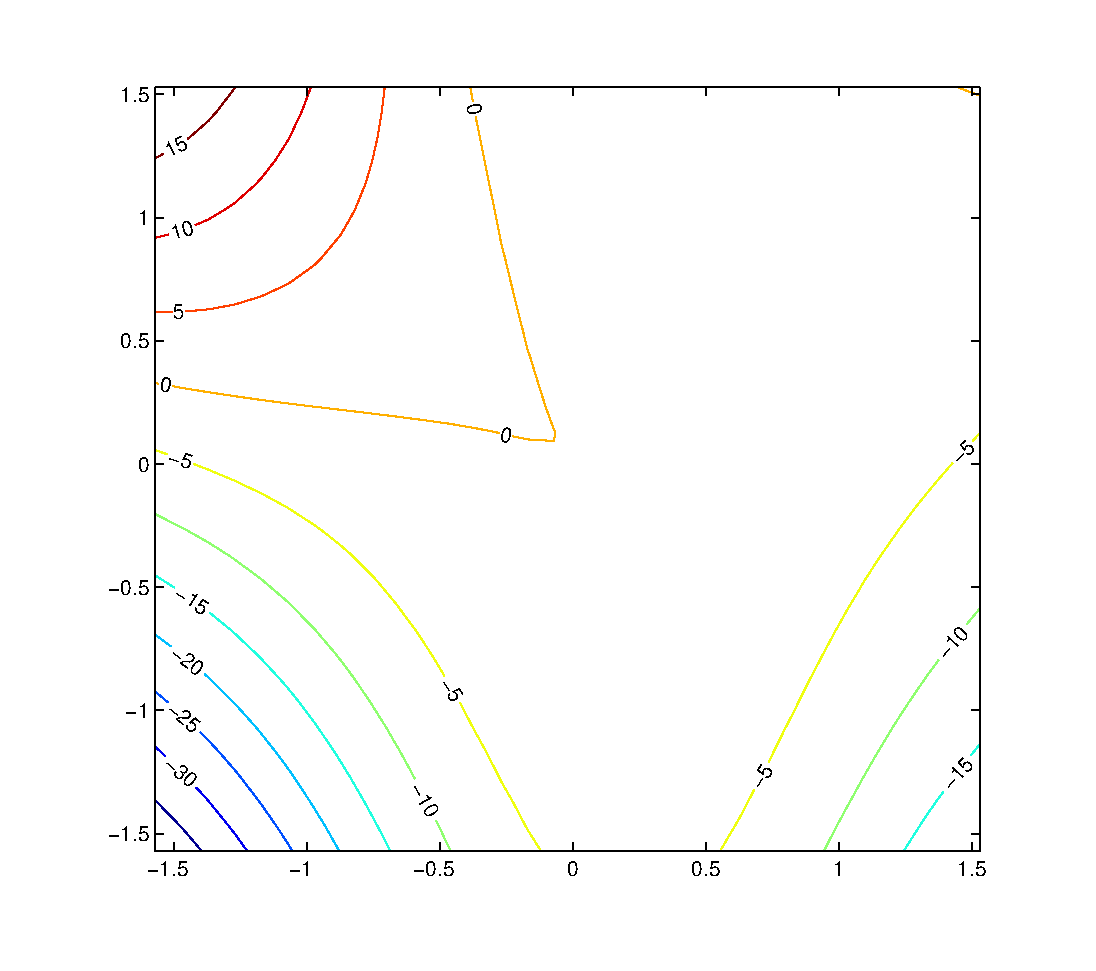
\includegraphics[width=10cm]{contour_V_dot}
	\caption{Região $D$ para diversos valores de $y$, tal que $\dot{V}(x) < y$}
	\label{fig:V_dot_levels}
\end{figure}

Como se vê na Figura \ref{fig:V_dot_levels}, a região para a qual $\dot{V}(x) < 0$, de fato, equivale à região abaixo da curva azul na Figura \ref{fig:reg_estab_Met4}.

Definida a região para a qual a análise de estabilidade é válida, estamos aptos a obter o domínio de atração para o caso apresentado no Método 1, que utiliza o modelo linearizado em torno da origem. Além das LMIs utilizadas para a análise de estabilidade vistas na Equação \ref{eq:LMIs_est_met_1}, é aplicado as condições \ref{eq:condition_1}--\ref{eq:enlargment_of_largest_set2} do Teorema \ref{th:reg_atrac_2}, de forma a se obter a melhor estimativa da região de atração. A matriz $P$ foi obtida, tal que
\begin{equation*}
P = \begin{bmatrix}0.6152&0.0000\\0.0000&0.4053\end{bmatrix}
\end{equation*}   

Como neste caso $P$ é constante, a região de atração será representada por uma região circular. Esta região é limitada no espaço $D$, no qual $\dot{V} < 0$, conforme pode ser observado na Figura \ref{fig:reg_atrac_met4}.

\begin{figure}[htbp]
	\centering
	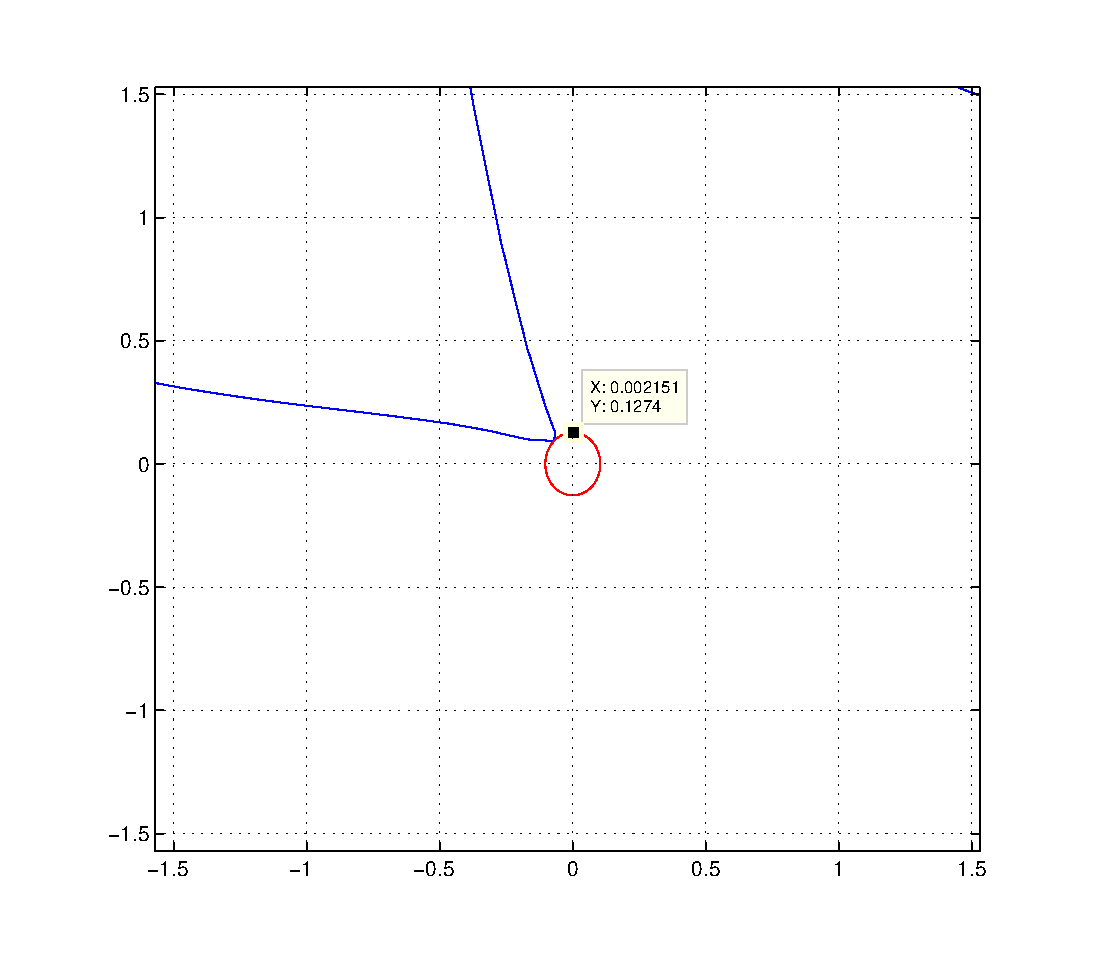
\includegraphics[width=10cm]{reg_atrac_method4}
	\caption{Estimativa da região de atração para dinâmica linearizada e $P$ constante}
	\label{fig:reg_atrac_met4}
\end{figure}

\subsection{Método 2: : (Boyd, 1994 \cite{bookboydl:1994}) Função de Lyapunov com $P$ constante e Teorema \ref{th:est_boyd}}

No capítulo anterior vimos que o modelo fuzzy Takagi-Sugeno do Exemplo \ref{example_LPJ12} somente é estável segundo o Teorema \ref{th:est_boyd} e com $\lambda = 20$ para o domínio $C_1 = 0.46C$, em que $C = \{x \in \rm I\!R^n | |x| \leq \pi/2\}$.

Como as LMIs para determinação da melhor estimativa do domínio de atração não interferem na condição de estabilidade, sabe-se que devem ser utilizadas as mesmas condições para se verificar a estabilidade que foram apresentadas no capítulo anterior por meio do Teorema \ref{th:est_boyd}. Assim, além das LMIs do Método 1 do capítulo anterior, com as condições já estabelecidas, as quais são $\lambda = 20$ e $C_1 = 0.46C$, resolveram-se também as LMIs \ref{eq:condition_1}--\ref{eq:enlargment_of_largest_set2} do Teorema \ref{th:reg_atrac_2}.

As simulações permitiram obter a matriz $P$, conforme segue.
\begin{equation*}
P = \begin{bmatrix}5.2598&0.0000\\0.0000&1.9153\end{bmatrix}
\end{equation*}

Para plotar a elipse que corresponde á superfície de nível da melhor estimativa da região de atração para este $P$ constante, utilizou-se a equação da elipse. Primeiramente determinou-se os parâmetros $b = P(1,2) = 0.0000$ e $c = P(2, 2) = 1.9153$. Além disso, assumiu-se $\gamma = 1$.
O comprimento do eixo maior a elipse equivale a $2*\sqrt(c/det(P))$, de forma que $max(x_1) = \sqrt(c/det(P)) = -min(x_1)$. Já o eixo menor foi obtido conforme a equação a seguir.
\begin{equation*}
x_2=-bx_1\pm \dfrac{\sqrt(c*\gamma-x1.^2*det(P))}{c}
\end{equation*}

A Figura \ref{fig:reg_atrac_Met1} mostra a região de estimativa do domínio de atração obtida para este método.

\begin{figure}[htbp]
	\centering
	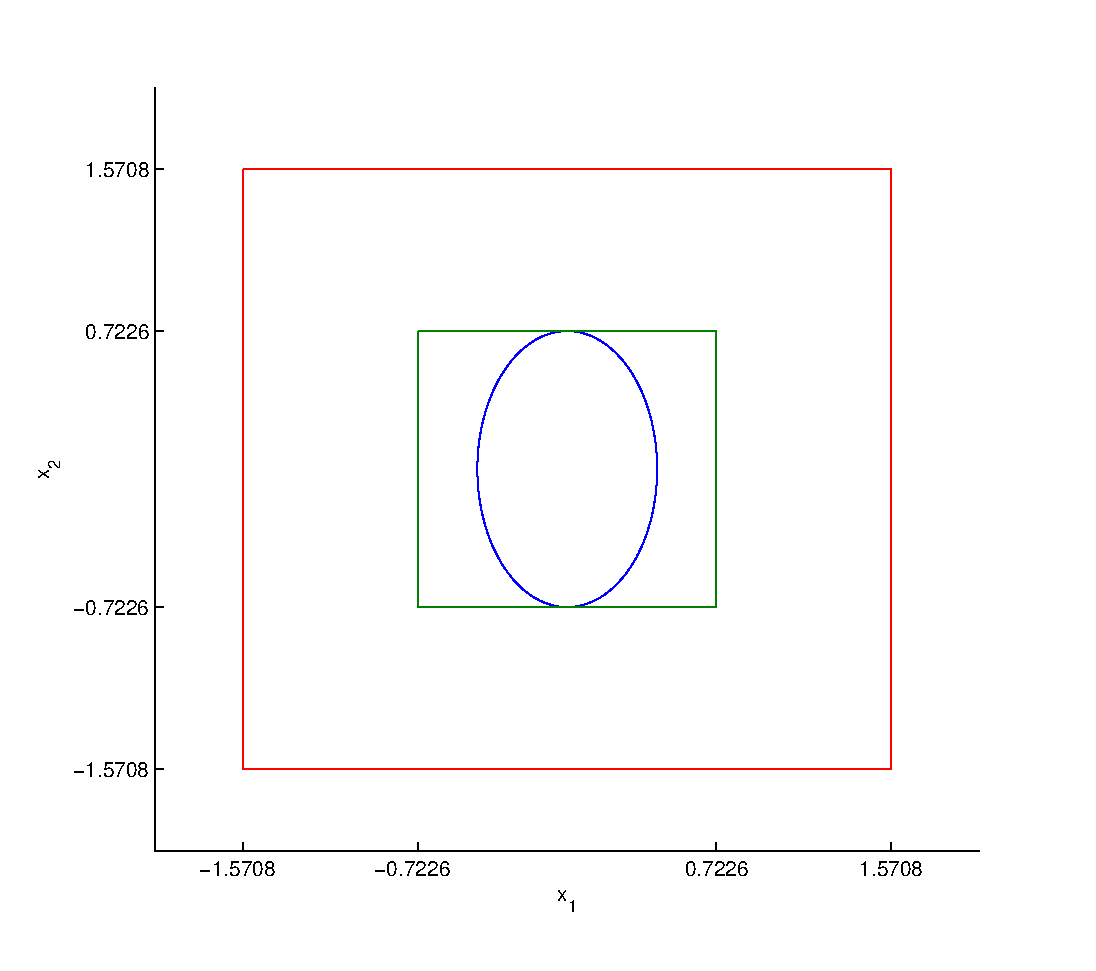
\includegraphics[width=10cm]{reg_atrac_Met1}
	\caption{Estimativa do domínio de atração do Exemplo \ref{example_LPJ12} com $\lambda = 20$ para o Método 2, curva em azul, domínio $C_1$ para a qual o sistema é localmente assintoticamente estável para este método, em verde, e domínio definido para os estados os sistema, em vermelho}.
	\label{fig:reg_atrac_Met1}
\end{figure}

\subsection{Método 3: (Mozelli, Palhares, Sousa e Mendes, 2009 \cite{MPSM:2009}) Função de  Lyapunov com $P$ dependente das funções de pertinência e limitante simples das derivadas do Teorema \ref{th:theorem_6}}

Conforme visto no capítulo anterior, este método de análise de estabilidade utiliza o artifício do limitante das derivadas simples. Os resultado obtidos previamente revelaram que a origem só é um ponto de equilíbrio estável para este método considerando-se apenas a região $C_2 = 0.51C$, em que $C = \{x \in \rm I\!R^n | |x| \leq \pi/2\}$, isto para $\lambda = 20$.

Para a obtenção da melhor estimativa da região de atração da origem para este método, consideraram-se as mesmas condições para as quais se garantiu estabilidade no capítulo anterior para $\lambda = 20$, isto é, considerou-se apenas o domínio contido em $C_2$. Assim, o sistema foi simulado para as LMIs que garantem a estabilidade para este método junto com as condições \ref{eq:condition_1}--\ref{eq:enlargment_of_largest_set2} do Teorema \ref{th:reg_atrac_2}, de forma que foram obtidas as matrizes $P_1$ e $P_2$ correspondentes aos vértices de $P(\alpha)$ conforme segue.

\begin{equation*}
P_1 =\begin{bmatrix}1.8537&0.7690\\0.7690&2.0013\end{bmatrix}\qquad P_2 = \begin{bmatrix}6.5500&-0.1329\\-0.1329&1.5609\end{bmatrix}
\end{equation*}

Por se tratarem de dois vértices, o domínio de atração agora não pode mais ser obtido conforme fora feito para os Métodos 1 e 2, que apresentavam $P$ constante, isto é, um único vértice de $P$. Assim, a curva de Lyapunov da estimativa do domínio de atração para este método foi obtida de forma tal que equivalesse à maior região contida pela interseção das superfícies de Lyapunov de cada vértice $P_i$. A Figura \ref{fig:reg_atrac_Met2} mostra esta região obtida.

\begin{figure}[htbp]
	\centering
	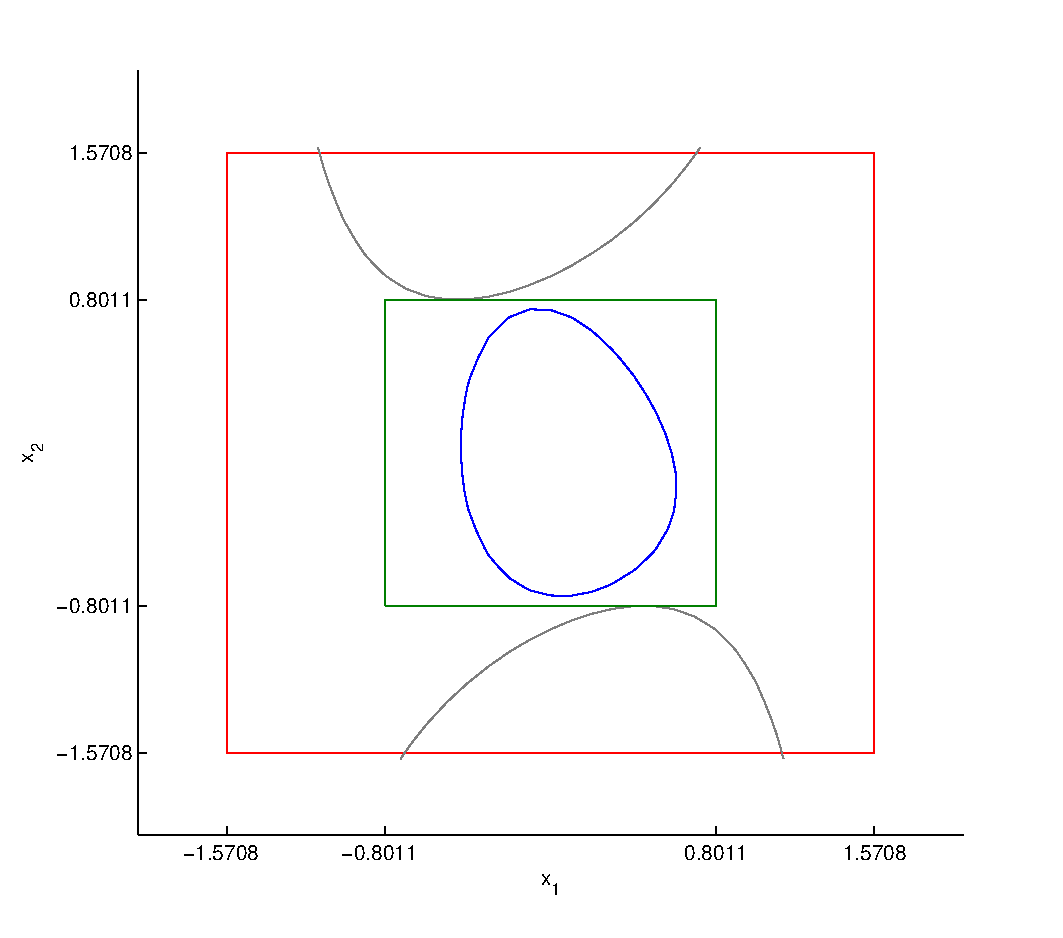
\includegraphics[width=10cm]{reg_atrac_Met2}
	\caption{Estimativa do domínio de atração do Exemplo \ref{example_LPJ12} com $\lambda = 20$ para o Método 3, curva em azul, domínio $C_2$ para a qual o sistema é localmente assintoticamente estável para este método, em verde, limitantes simples das derivadas das funções de pertinência, em cinza, e domínio definido para os estados os sistema, em vermelho}.
	\label{fig:reg_atrac_Met2}
\end{figure}

\subsection{Método 4: (Método Proposto) Função Lyapunov com $P$ dependente das funções de pertinência e Teorema \ref{th:reg_atrac_1}}

Para este Método, a melhor estimativa do domínio de atração para o Exemplo \ref{example_LPJ12} foi obtida obtendo $P$ definido positivo que satisfizesse as condições do Teorema \ref{th:reg_atrac_1}, considerando-se $\omega_1$ = $\omega_2$ = 1, de forma que se obtiveram-se os vértices $P_1$ e $P_2$ de $P(\alpha)$, conforme segue.
\begin{equation*}
P_1 = 1.0e+05 \begin{bmatrix} 0.3085&0.4474\\0.4474&2.1328\end{bmatrix}\qquad P_2 = 1.0e+05 \begin{bmatrix}1.8249& 0.1148\\ 0.1148&1.2450\end{bmatrix}
\end{equation*}

Este método tem em especial o fato de que a estimativa da região de atração é plotada para um $\gamma = 1.9666e-05$, obtido da resolução das LMIs do Teorema \ref{th:reg_atrac_1}, ao contrário do que ocorre para os demais Métodos, em que se assume $\gamma = 1$.

A Figura \ref{fig:reg_atrac_met5} apresenta a superfície da melhor estimativa do domínio de atração para o Método 5.

\begin{figure}[htbp]
	\centering
	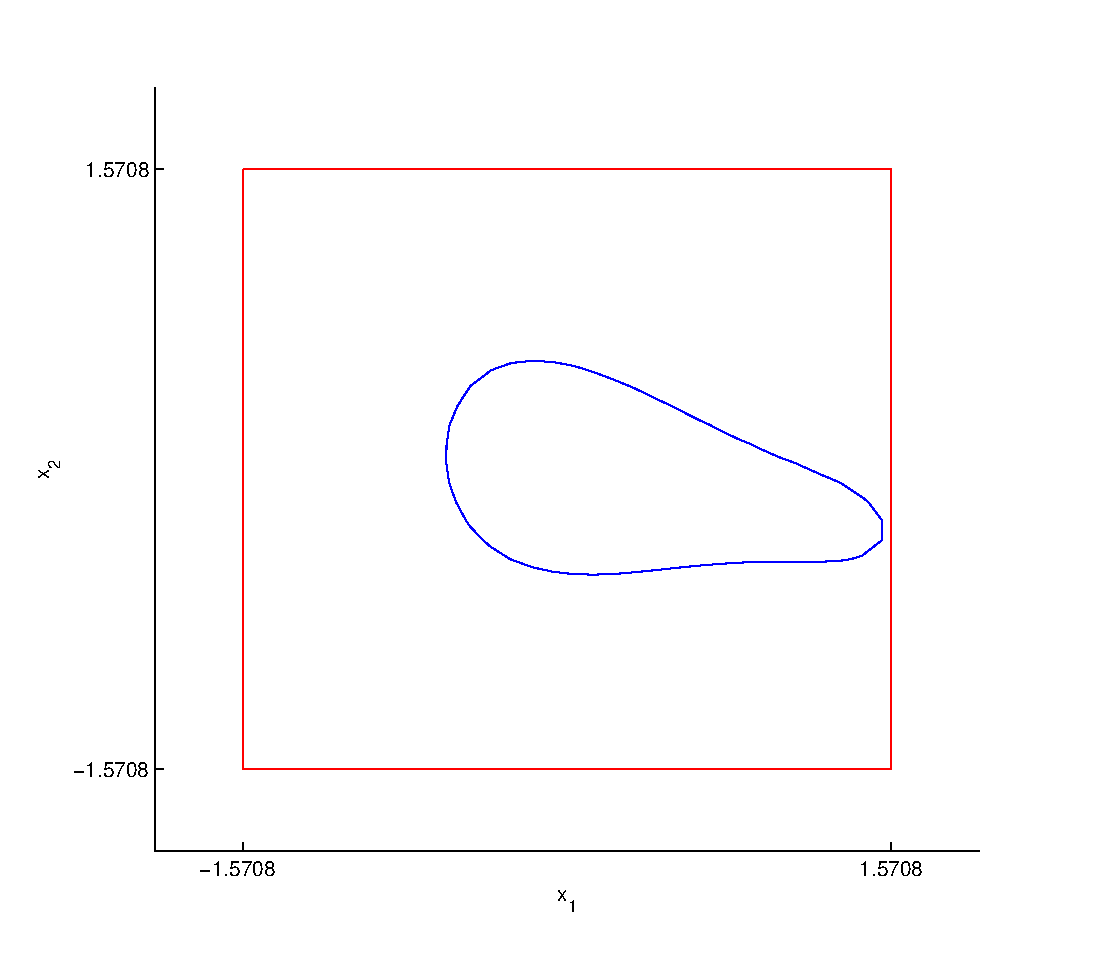
\includegraphics[width=10cm]{reg_atrac_Met5}
	\caption{Estimativa do domínio de atração do Exemplo \ref{example_LPJ12} com $\lambda = 20$ para o Teorema~\ref{th:reg_atrac_1}, curva em azul, e domínio $C$ para a qual o sistema é localmente assintoticamente estável para o Resultado Principal (Proposto), em vermelho}
	\label{fig:reg_atrac_met5}
\end{figure}

\subsection{Método 5: (Método Proposto) Função Lyapunov com $P$ dependente das funções de pertinência e Teorema \ref{th:reg_atrac_2}}

A melhor estimativa do domínio de atração para o Exemplo \ref{example_LPJ12}, assumindo-se $\lambda = 20$, para o Resultado Principal deste trabalho é obtida resolvendo-se as LMIs propostas no Teorema~\ref{th:reg_atrac_2}. Obtendo-se mais uma vez o resultado o qual indica que a origem é um ponto estável, gerando-se valores para os vértices de $P(\alpha)$ definido positivo.

Como $P(\alpha)$ é dependente das funções de associação, este possui $2$ vértices, os quais são descritos a seguir, considerando-se a condição de melhor estimativa do domínio de atração, ou seja, obtendo solução tal que satisfizesse o Teorema \ref{th:reg_atrac_2}.
\begin{equation*}
P_1 =\begin{bmatrix}0.4596&0.3295\\0.3295&1.9980\end{bmatrix}\qquad P_2 = \begin{bmatrix}1.9137&-0.1639\\-0.1639&0.4671\end{bmatrix}
\end{equation*}

A curva correspondente á melhor estimativa do domínio de atração para este método foi obtida conforme descrito no Método 2. Foi obtida a região correspondente à maior interseção entre as elipses equivalentes aos vértices de $P(\alpha)$. A Figura \ref{fig:reg_atrac_Met3} apresenta o resultado obtido para o domínio de atração obtido para este método.

\begin{figure}[htbp]
	\centering
	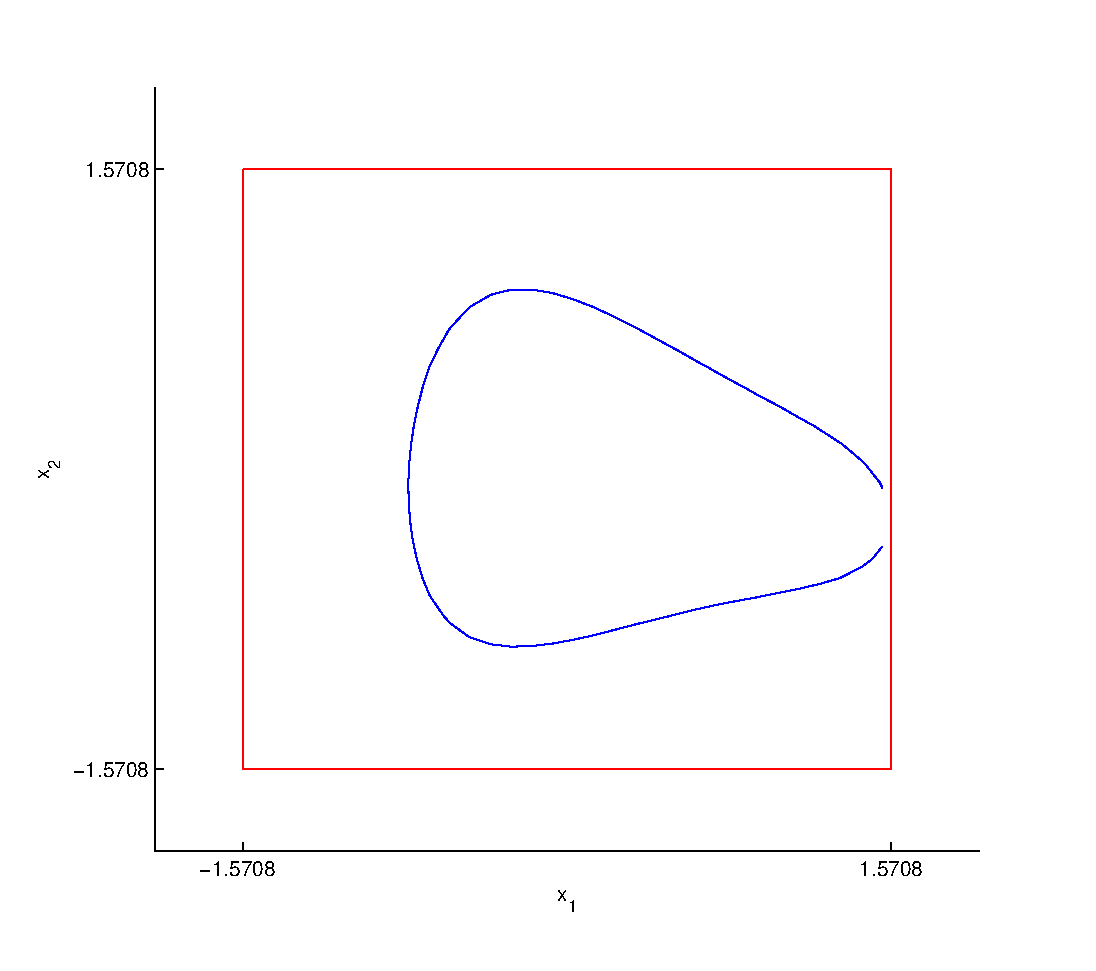
\includegraphics[width=10cm]{reg_atrac_Met3}
	\caption{Estimativa do domínio de atração do Exemplo \ref{example_LPJ12} com $\lambda = 20$ para o Resultado Principal (Proposto), curva em azul, e domínio $C$ para a qual o sistema é estável para este método, em vermelho}.
	\label{fig:reg_atrac_Met3}
\end{figure}

\subsection{Comparação entre os métodos}

Para se comparar os resultados dos cinco métodos apresentados nesta seção, como nem todas as curvas obtidas têm um formato definido como elipse ou círculo, o que dificulta os cálculos da área contida pela curva de Lyapunov obtida para cada um dos métodos, as curvas correspondentes a estas estimativas da região de atração serão plotadas em um único gráfico, de forma a se verificar visualmente qual delas cobre uma maior região no plano de estados, conforme mostra a Figura \ref{fig:reg_atrac_all_met}.


\begin{figure}[htbp]
	\centering
	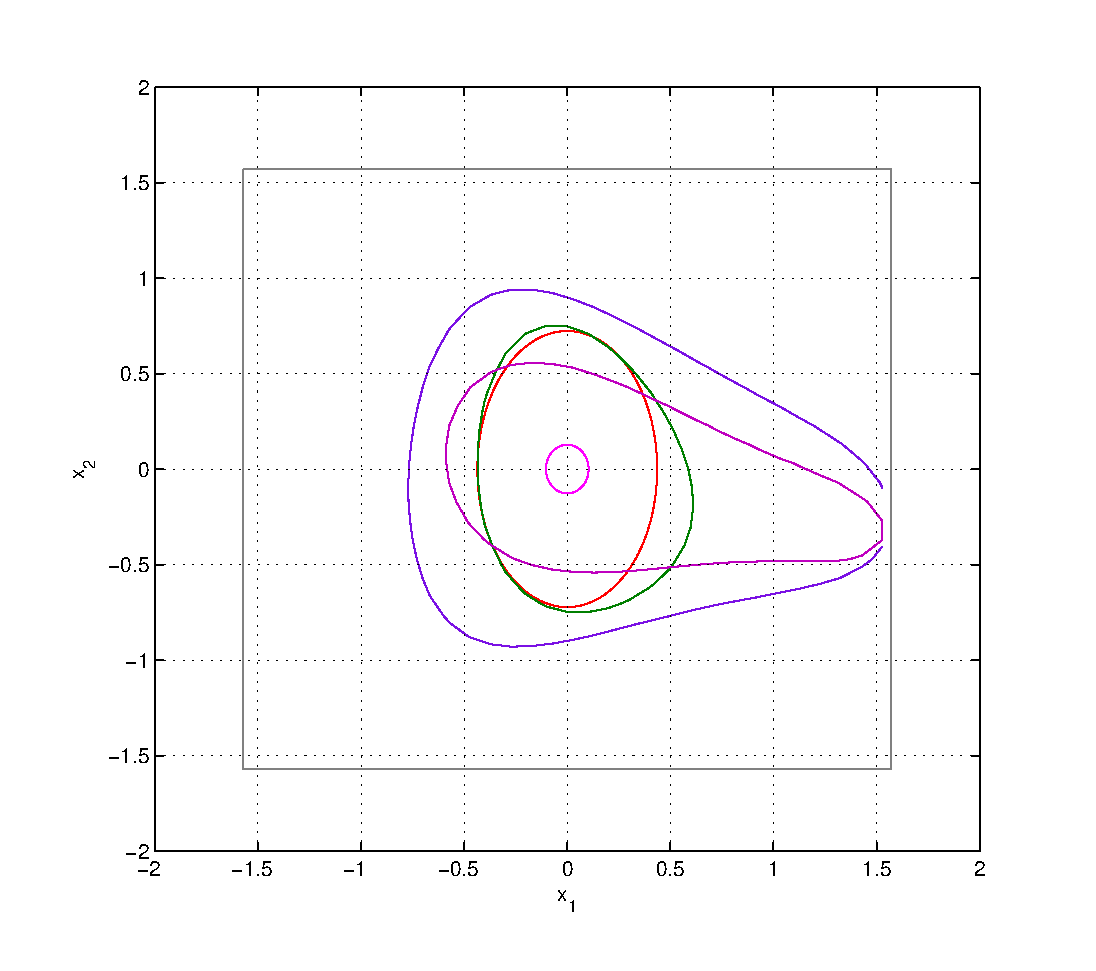
\includegraphics[width=10cm]{domain_of_attraction_all_methods}
	\caption{Estimativa do domínio de atração do Exemplo \ref{example_LPJ12} com $\lambda = 20$ para os cinco Métodos propostos nesta seção. A curva referente ao Método 1 é mostrada na cor rosa. A curva em vermelho corresponde ao  Método 2, a curva em verde equivale ao  Método 3. A curva obtida do  Método 4 aparece em roxo e curva do  Método 5, em azul. A região $C$ para a qual os estados são limitados aparece na cor cinza}
	\label{fig:reg_atrac_all_met}
\end{figure}

Na Figura \ref{fig:reg_atrac_all_met}, a região para a qual os estados estão limitados aparecem como o quadrado na cor cinza. As regiões de atração do ponto de equilíbrio na origem aparecem para os Métodos 1, 2, 3, 4 e 5 aparecem na Figura, respectivamente, nas cores rosa, vermelho, verde, roxo e azul.

O Método 1, apresentado na cor rosa, foi o que gerou o pior resultado, o que se era esperado, uma vez que a dinâmica linearizada neste método só é válida para regiões muito próximas á origem, já que o sistema foi linearizado em torno deste ponto. Todos os demais métodos foram aplicados para a dinâmica do sistema modelada segundo a estratégia de não linearidade por setor para modelos fuzzy Takagi-Sugeno.

O Método 3, que utiliza artifício dos limitantes por derivada simples se mostrou um pouco melhor que o Método 2, o qual apresenta $P$ constante. 

Ao contrário do que fora feito para os Métodos 1, 2 e 3, em que se utilizou apenas o Teorema \ref{th:reg_atrac_2} para a obtenção da melhor estimativa de região de atração, para o Resultado principal deste trabalho, obteve-se a estimativa de região de atração utilizando tanto o Teorema \ref{th:reg_atrac_1}, conforme mostra o Método 4, quanto para o Teorema \ref{th:reg_atrac_2}, segundo Método 5.
Como se pode observar na Figura \ref{fig:reg_atrac_all_met}, o método que gerou o melhor resultado para estimativa da região de atração foi o  Método 5, que equivale ao Resultado Principal proposto por este trabalho utilizando-se o Teorema  \ref{th:reg_atrac_2} e o Método 4 gerou o segundo melhor resultado. 

% \section{Exemplos}

% [UFSM]

\section{Considerações Finais}

Neste capítulo foram apresentados dois Teoremas para a obtenção da melhor estimativa de região de atração do ponto de equilíbrio situado na origem do plano de estados para sistemas dinâmicos não lineares modelados segundo o artifício de não linearidade por setor local, proposto por \cite{booktw:2003}, para obtenção de modelos fuzzy Takagi-Sugeno do sistema \cite{articlets:1985}. Tentou-se obter a maior região dentro do espaço de estados para a qual o sistema é estável e para a qual, uma vez que as respostas, iniciadas em qualquer ponto da região do plano de estado limitada pelas restrições dos estados do sistema, adentrem esta região de atração, jamais consiga sair desta.

Para verificar se, de fato, o Resultado Principal (Proposto) neste trabalho fornecia o melhor resultado para a estimativa do domínio de atração do ponto de equilíbrio na origem, utilizaram-se outros três métodos. Dois destes métodos já haviam sido explorados no capítulo anterior, em que se analisou a estabilidade de pontos de equilíbrio para sistemas com dinâmica fuzzy T-S e o outro método consistiu na análise de estabilidade e obtenção da estimativa de região de atração para o sistema linearizado em torno da origem.

O primeiro Método utilizado para comparação consistiu no modelo linearizado em torno da origem e com $P$ constante. Este método, embora tenha se apresentado como estável para toda a região definida para os estados do sistema, produz o pior resultado de estimativa de região de atração, obtida com o uso do Teorema \ref{th:reg_atrac_2}, dado que só é válido para regiões muito próximas à origem, como se verificou varrendo-se a região para a qual relação $\dot{V} < 0 $ é válida para o sistema não linear.

Para dois métodos já vistos no capítulo anterior, com exceção do Resultado Principal (Proposto), que utilizam Estabilidade de Lyapunov com P constante, proposto por (Boyd, 1994 \cite{bookboydl:1994}) e Estabilidade de Lyapunov com $ P(\alpha)$ e limitante por derivada simples, segundo proposto por (Mozelli, Palhares, Sousa e Mendes, 2009 \cite{MPSM:2009}), respectivamente, foram obtidas as estimativas de região de atração utilizando-se o Teorema \ref{th:reg_atrac_2}. Este primeiro Método se mostrou pior que o segundo, uma vez que a região estimada foi menor. Porém, ambos apresentaram resultados piores que os do Teorema \ref{th:main_result}, que consiste no resultado principal deste trabalho. Estes resultados foram piores, tanto quando comparados utilizando-se o Teorema \ref{th:reg_atrac_1}, quanto o Teorema \ref{th:reg_atrac_2} para a estimativa da região de atração. 

Para o caso dos Métodos 4 e 5, correspondentes ao resultado principal, o que gerou o melhor resultado, que se permitiu obter a maior estimativa de região de atração dentre todos os métodos vistos, foi o Método 5.

% *** Conclusões
\chapter{Conclusões}\label{CapConclusoes}

Neste trabalho foi feito o estudo da análise estabilidade de sistemas não-lineares por meio do Teorema de estabilidade de Lyapunov via LMIs. Inicialmente considerou-se o sistema com dinâmica não-linear, a partir do qual se obteve o retrato de fase do sistema para a região no espaço de estados. A partir do retrato de fase foi possível verificar qualitativamente o comportamento dos pontos de equilíbrio do sistema, podendo-se classificá-los, dentre outros, em estável, assintoticamente estável e instável. O ponto de equilíbrio é estável quando as trajetórias de resposta para diferentes pontos iniciais sempre se aproximam para uma região próxima ao ponto de equilíbrio. Quando as trajetórias tendem ao ponto de equilíbrio à medida que o tempo tende ao infinito, este ponto é dito como assintoticamente estável. Caso as trajetórias se afastem, o ponto é dito como instável. Este princípio foi utilizado no decorrer do trabalho para se classificar analisar a estabilidade de pontos de equilíbrio.

Em seguida, foi obtido o modelo fuzzy Takagi-Sugeno dos sistemas não-lineares em estudo e verificou-se que esta modelagem representa o modelo linearizado de forma exata. Obtida esta modelagem, que consiste no conjunto de sistemas linearizados associados na forma de vértices, iniciou-se tópico principal deste projeto, que consistiu na análise de estabilidade e na estimativa da região de atração para pontos de equilíbrio na origem. Utilizou-se o artificio de mudança de variável para deslocar o ponto de equilíbrio do sistema para a origem, sem que houvesse perda de generalidade, de forma a se abranger um número maior de sistemas.

No capítulo sobre análise de estabilidade utilizou-se o Teorema de Estabilidade de Lyapunov, LMIs e o Teorema de Finslar para se propor um novo Teorema de análise de estabilidade de sistemas fuzzy T-S modelados segundo a técnica de não-linearidade por setor local. O objetivo com a proposta deste Teorema foi obter condições menos conservadoras, tais que a análise de estabilidade garantisse resultados mais abrangentes. Fez-se uso de outros métodos já existentes na literatura para serem comparados com o método aqui proposto.

As comparações do método proposto neste trabalho com os métodos encontrados na literatura permitiram ver que o nosso método gera melhores resultados para um valor fixo de $\lambda = 20$, visto que foi o único que garantiu a estabilidade em toda a região $C$ para a qual o sistema é definido. Fixando-se a região de análise em todo o domínio $C$, variou-se o valor de $\lambda$ até se obter os valores tais que as LMIs necessárias para a estabilidade não gerassem resultado. Assim, verificou-se que o nosso método foi o melhor quando analisado o limitante superior, uma vez que fora o único para o qual se verificou que não há limitante superior de $\lambda$ para o qual a origem deixe de ser estável para a região $C$. Já para o limitante inferior, o nosso método gerou o pior resultado.

Mantendo-se $\lambda = 20$, foi feito uma estimativa da região de atração para os métodos utilizados até agora, utilizando-se o mesmo critério de maximização para todos. Verificou-se que o nosso método gera o melhor resultado para esta estimativa. Foi sugerido um novo teorema para a maximização da estimativa da região de atração, o qual não foi bem sucedido.

Como trabalhos futuros sugere-se:
\begin{enumerate}
\item Comparar com métodos mais recentes na literatura;
\item Alterar os valores dos pesos $\omega_1$ e $\omega_2$ do Teorema \ref{th:reg_atrac_1} para se obter uma melhor estimativa de região de atração por meio deste;
\item Aumentar os graus dos simplexes para os vértices P e X do resultado principal, em busca de melhores resultados.
\end{enumerate}

%%%%%%%%%%%%%%%%%%%%%%%%%%%%%%%%%%%%%%%%%%%%%%%%%%%%%%%%%%%%%%%%%%%%%%%%%
% Referencias bibliograficas
%%%%%%%%%%%%%%%%%%%%%%%%%%%%%%%%%%%%%%%%%%%%%%%%%%%%%%%%%%%%%%%%%%%%%%%%%
\bibliographystyle{abnt-num} % use este estilo para ABNT numerico
%\bibliographystyle{abnt-alf} % use este estilo para ABNT alfa-numerico
\renewcommand{\bibname}{REFERÊNCIAS BIBLIOGRÁFICAS}
\addcontentsline{toc}{chapter}{REFERÊNCIAS BIBLIOGRÁFICAS}
\bibliography{relatorio}

%%%%%%%%%%%%%%%%%%%%%%%%%%%%%%%%%%%%%%%%%%%%%%%%%%%%%%%%%%%%%%%%%%%%%%%%%
% Anexos
%%%%%%%%%%%%%%%%%%%%%%%%%%%%%%%%%%%%%%%%%%%%%%%%%%%%%%%%%%%%%%%%%%%%%%%%%
\anexos
\makeatletter % não retirar estes comandos
\renewcommand{\@makechapterhead}[1]{%
  {\parindent \z@ \raggedleft \setfontarial\bfseries 
        \LARGE \thechapter. \space\space 
    \uppercase{#1}\par
    \vskip 40\p@
  }
}
\makeatother

%%TCIDATA{LaTeXparent=0,0,relatorio.tex}

\chapter{\textit{Plot} Retrato de Fase\label{AnEsquematicos}

x1 = x1\_min:x1\_step:x1\_max;

x2 = x2\_min:x2\_step:x2\_max;

[X1,X2] = meshgrid(x1,x2);

F1= f1(X1, X2);

F2= f2(X2, X2);

hold off

figure;clf

streamslice(X1,X2,F1,F2,2); \% https://www.mathworks.com/help/matlab/ref/streamslice.html

xlabel('x\_1');ylabel('x\_2');

line([0],[0],'marker','o','linestyle','none','markerfacecolor','r') \%plots origin as equilibrium point

hold off;

\chapter{Plot Condi��o de Inclus�o (Estimativa de regi�o de atra��o) para P constante\label{AnEsquematicos

function level\_curve(P, gamma, color)

\%Plots the level curve V(x) = x'*P*x = gamma, given P and gamma.

for i = 1:length(P)


if length(P) > 1



Pi = P{i{1;
else
Pi = P{i;
end
%a = Pi(1,1);
b = Pi(1,2); % = Pi(2,1);
c = Pi(2,2);
dP = det(Pi);

%[V,D] = eig(Pi);
%v1=V(:,1);
%v2=V(:,2);
%figure;plot(v1(1),v1(2),'r*',v2(1),v2(2),'b*');
%hold on

%Calculo
x1max=sqrt(c*gamma/dP);
steps = (2*x1max)/1e4;
x1=-x1max:steps:x1max;
x2a=($-b*x1+sqrt(c*gamma-x1.^2*dP))/c$;
x2b=($-b*x1-sqrt(c*gamma-x1.^2*dP))/c$;

%Plot
hold on
plot(x1,x2a,color)
plot(x1,x2b,color)
hold off
grid
volume = det(inv(Pi)*gamma); 
end
end

%\refstepcounter{noAnexo}

\end{document}

